\documentclass[8pt]{beamer}

\usetheme[numbering=fraction, progressbar=foot, block=fill]{metropolis}
%\usecolortheme{seahorse}

\makeatletter
\setlength{\metropolis@titleseparator@linewidth}{1pt}
\setlength{\metropolis@progressonsectionpage@linewidth}{2pt}
\setlength{\metropolis@progressinheadfoot@linewidth}{2pt}
\makeatother

\usepackage{appendixnumberbeamer}
\usepackage{booktabs}
\usepackage{pgfplots}
\usepackage{tikz}
\usepackage{multicol}
\usepackage{changepage}
\usepackage{hyperref}
\usepackage{makecell}
\usepackage{multirow}
\usepackage{arydshln}
\usepackage{mathtools}
\usepackage{graphicx}
\usepackage[document]{ragged2e}
\usepgfplotslibrary{dateplot}
\usepackage{xspace}

\newcommand{\themename}{\textbf{\textsc{metropolis}}\xspace}

% ================== Customization
\definecolor{mygreen}{RGB}{40,85,175} %Dark green
\definecolor{myred}{RGB}{153,26,0} %Dark red
\definecolor{myblue}{RGB}{66,98,163} %Dark blue
\definecolor{mycolor}{RGB}{66,98,163}

\setbeamercolor{background canvas}{bg=white}

%\setbeamertemplate{blocks}[rounded][shadow=false]

% ================== Title page
\title{Search for dark matter production in association with top quarks in the dilepton final state at $\sqrt{s} = $ 13 TeV}
%\subtitle{The subtitle goes here}
%\date{\today}\newcommand{\themename}{\textbf{\textsc{metropolis}}\xspace}

% ================== Customization
\definecolor{mygreen}{RGB}{40,85,175} %Dark green
\definecolor{myred}{RGB}{153,26,0} %Dark red
\definecolor{myblue}{RGB}{66,98,163} %Dark blue
\definecolor{mycolor}{RGB}{66,98,163}

\setbeamercolor{background canvas}{bg=white}

%\setbeamerfont{institute}{series=\bfseries,parent=structure}
\setbeamerfont{institute}{size=\large}
\setbeamerfont{author}{size=\normalsize}
\setbeamerfont{date}{size=\normalsize}
%\setbeamertemplate{frame footer}{\footnotesize \insertshortauthor~(\insertshortinstitute)}
\setbeamerfont{page number in head/foot}{size=\small}
\setbeamerfont{frametitle}{size=\normalsize}

\newcommand{\backupbegin}{
   \newcounter{finalframe}
   \setcounter{finalframe}{\value{framenumber}}
}
\newcommand{\backupend}{
   \setcounter{framenumber}{\value{finalframe}}
}

%\setbeamertemplate{blocks}[rounded][shadow=false]

%\subtitle{The subtitle goes here}
%\date{\today}
%\date{}
%\author{\justifying Afiq Anuar, Alexander Grohsjean, Christian Schwanenberger, Dominic Stafford, Nicole Stefanov (1), Kristian Hahn, Kevin Sung (2), Pablo Martinez Ruiz Del Arbol, J\'{o}natan Piedra,  \textbf{C\'{e}dric Prieels (3)}, Deborah Pinna, Victor Shang (4)}
%\institute{\textbf{\textbf{January 8th 2021}} \\ 
%\begin{multicols}{2}
%\normalsize{(1) DESY} \\
%(2) NorthWestern University \\
%(3) Instituto de Fisica de Cantabria \\
%(4) University of Wisconsin
%\end{multicols}}
%
%\titlegraphic{
%   \tikz[overlay,remember picture]
%       \node[at=(current page.south east), anchor=south east] {
%           
\includegraphics[height=1cm]{figs/desy.png}\hspace{18pt}
\includegraphics[height=1.1cm]{figs/northwestern.png}\hspace{18pt}
\includegraphics[height=0.9cm]{figs/ifca.jpg}\hspace{18pt}
\includegraphics[height=1cm]{figs/wisconsin.png}\hspace{18pt}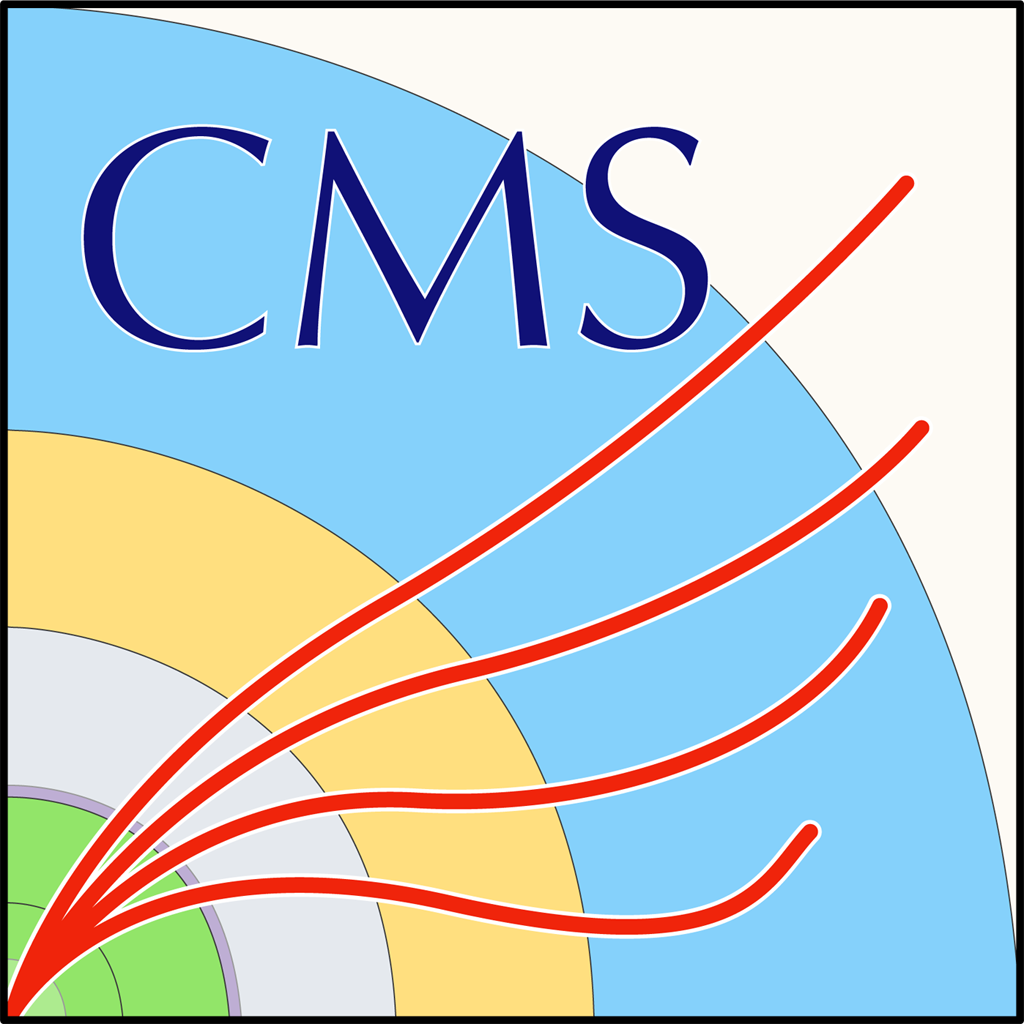
\includegraphics[height=1cm]{figs/cms.jpg}
%       };
%}

\date{\vspace{-3pt}February 22th 2021}
\author{Pablo Mart\'{i}nez Ru\'{i}z del \'{A}rbol, J\'{o}natan Piedra Gomez, \textbf{C\'{e}dric Prie\"{e}ls}}
\institute{Instituto de F\'{i}sica de Cantabria}

\titlegraphic{
   \tikz[overlay,remember picture]
       \node[at=(current page.south east), anchor=south east] {
           
\includegraphics[height=1.0cm]{figs/ifca_final.png}\hspace{18pt}
\includegraphics[height=1.2cm]{figs/uc.jpg}\hspace{8pt}
\includegraphics[height=1.4cm]{figs/csic.jpg}\hspace{8pt}
\includegraphics[height=1.2cm]{figs/maetzu.png}\hspace{8pt}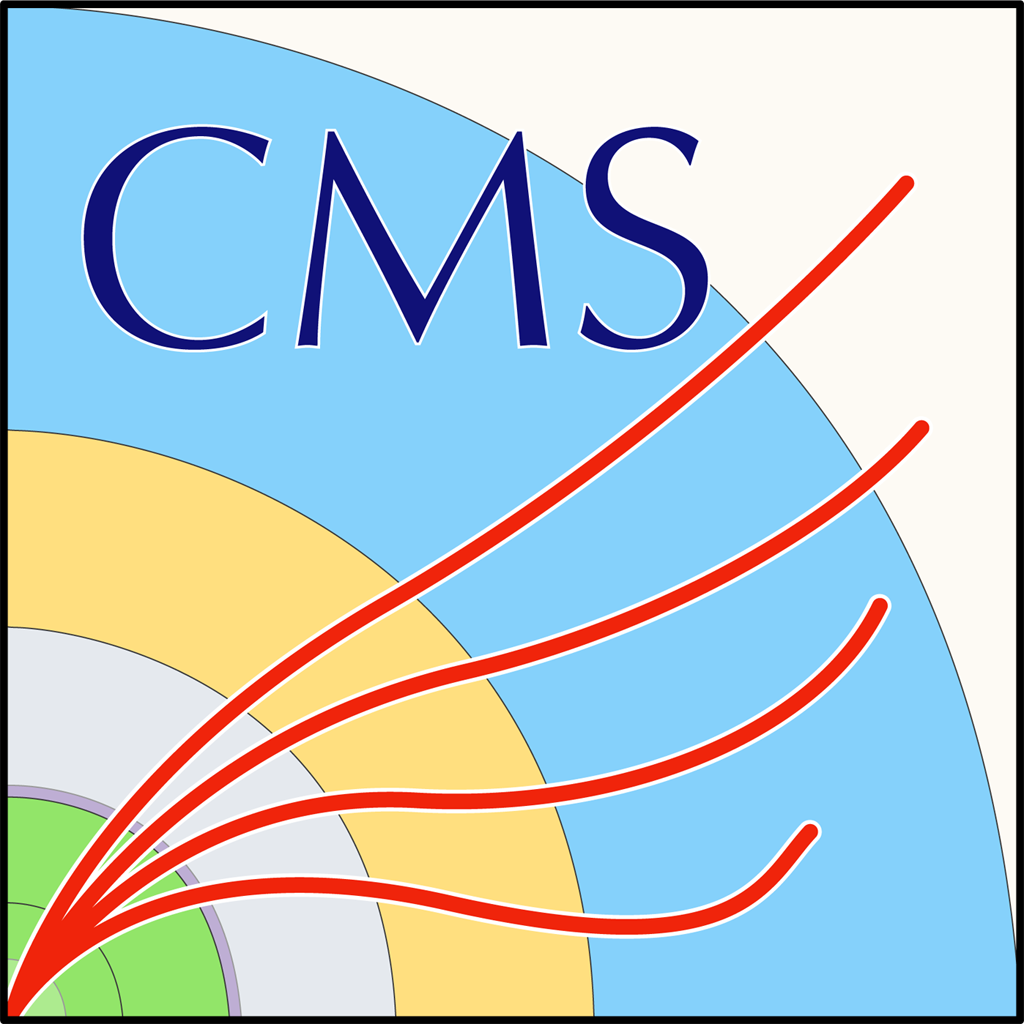
\includegraphics[height=1.2cm]{figs/cms.jpg}
       };
}

% ================== Document
\begin{document}

\maketitle

\begin{frame}{Outline}
\justifying
\begin{itemize}
\item Introduction
\item The dark matter case
\item The experimental setup
\begin{itemize}
\item The LHC accelerator
\item The CMS detector
\end{itemize}

\item Global strategy
%\item Event reconstruction
\item Data, signals and backgrounds
\item Event selection
\item Signal extraction
\item Systematic uncertainties
\item Results and interpretation
\item Conclusions
\end{itemize}
\end{frame}

\begin{frame}{Introduction}
\justifying
A search for the \alert{production of dark matter particles in association with either one or two top quarks} is presented:

\vspace{-5pt}
\begin{itemize}
\justifying
\item We study the $pp$ collisions produced by the LHC at $\sqrt{s} = 13$ TeV;
\item Reconstruction performed by the CMS detector;
\item Legacy analysis, considering the full Run II dataset (data collected in 2016, 2017 and 2018 and summing around 137 fb$^{-1}$).
\end{itemize} \vfill

\begin{block}{\centering Motivation}\end{block}
\vspace{-5pt}
\begin{itemize}
\justifying
\item Several (mostly astrophysical) evidences for the existence of dark matter, but \textbf{no direct nor direct detection} so far;
\item We hope to be able to produce such particles in the high energy collisions produced by the LHC if they exist.
\end{itemize} \vfill

\begin{block}{ \centering Main objective}\end{block}
\vspace{-5pt}
\begin{itemize}
\justifying
\item Consider different dark matter production models to eventually exclude some of them or at least \textbf{put upper limits on their cross section of production}.
\end{itemize} \vfill
\end{frame}








\begin{frame}[standout]
The dark matter case
\end{frame}

\begin{frame}{The Standard Model}
\justifying
The most accepted model to describe the elementary particles and some of the fundamental interactions between them is the \alert{Standard Model}:

\begin{itemize}
\justifying
\item Contains 26 free parameters, among which the masses of the \textbf{12 predicted fermions};
\item Many \textbf{successful predictions} made over the years, such as the existence of the top quark, and the W, Z and Higgs bosons \cite{SMPredictions}.
\end{itemize} \vfill

\begin{figure}[htbp]
\begin{center}
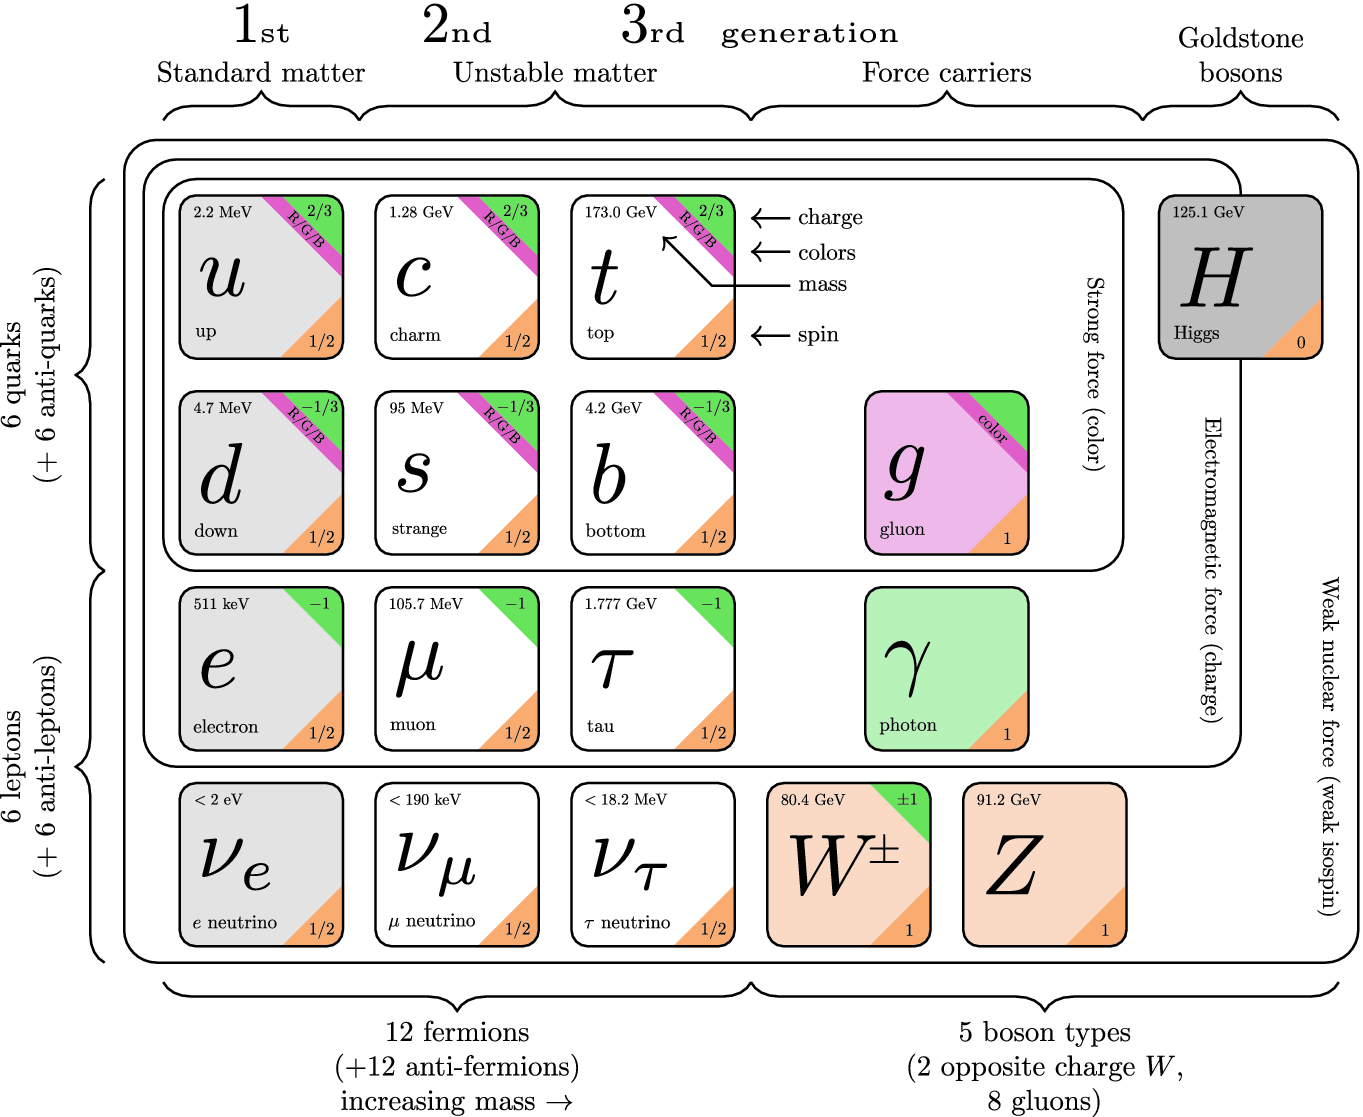
\includegraphics[width=5.2cm, height=4cm]{figs/SMFermions.png}
\end{center}
\end{figure} \vfill

However, this model \alert{has several shortcomings}: eventual exotic particles which do not fit within this model (such as dark matter) are extensively searched for nowadays. \vfill
\end{frame}

\begin{frame}{At the origins of dark matter I}
\justifying
The concept of dark matter can be traced back to the 19th century, and was introduced to \alert{explain several astrophysical evidences}, among which: \vfill

\vspace{10pt}	
\begin{block}{ \centering Zwicky's calculations}\end{block}

\begin{itemize}
\justifying
\item Measurement of the mass of the Coma Cluster using the virial theorem;
\item Concluded that its mass was \textbf{400-500 times larger} than the value obtained by Hubble, considering only visible galaxies \cite{Zwicky}.
\end{itemize} \vfill

\vspace{10pt}	
\begin{block}{ \centering Spiral galaxies rotation curves}\end{block}

\begin{columns}
	\begin{column}{0.65\textwidth}
\begin{itemize}
\justifying
\vspace{-5pt}	
\item Stars within spiral galaxies should rotate with a velocity depending on the radius to the galactic center, but \textbf{this is not what is observed experimentally} \cite{RotationCurves};
\vspace{1pt}	
\item Either our understanding of gravity at large scales or our basic understanding of galaxies as a celestial body made of stars has to be revised.
\end{itemize} 
\end{column}

\begin{column}{0.44\textwidth}
\begin{figure}[htbp]
\begin{center}
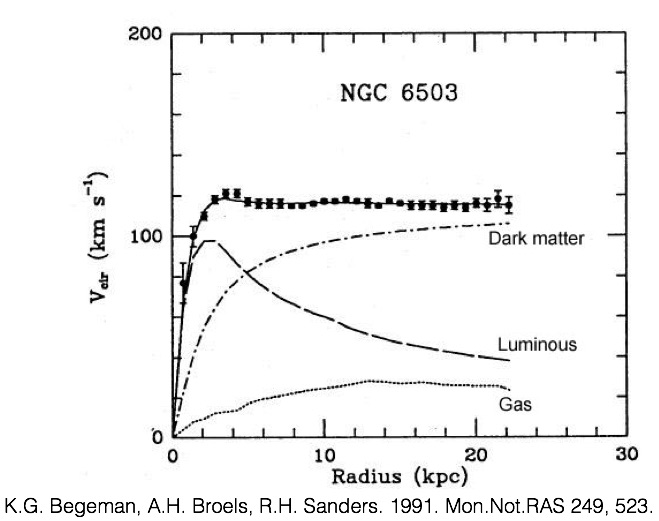
\includegraphics[width=4.5cm, height=3.7cm]{figs/RotationCurve.jpeg}
\end{center}
\end{figure}
\end{column}
\end{columns} \vfill

\end{frame}

\begin{frame}{At the origins of dark matter II}
\justifying

\vspace{5pt}
\begin{block}{ \centering CMB anisotropies}\end{block}

\begin{itemize}
\justifying
\item Background of primary radio waves emitted when the Universe became transparent around 380 000 years after the Big Bang;
\item Can be considered as emitting a black body spectrum with a temperature of $(2.72548\pm 0.00057)$K \cite{CMBTemperature}, but small anistropies at the $10^{-5}$ level are observed;
\item Implies that dark matter \alert{accounts for $\sim 27\%$ of the total mass of the Universe}.
\end{itemize} \vfill

\begin{columns}
	\begin{column}{0.54\textwidth}
\begin{figure}[htbp]
\begin{center}
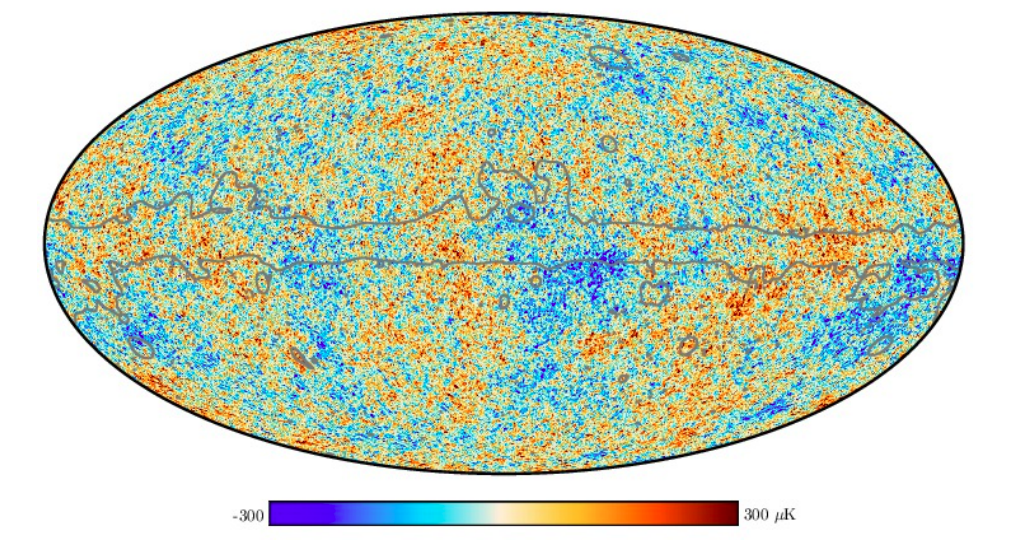
\includegraphics[width=6.5cm, height=3cm]{figs/PlanckTemperature.png}
\end{center}
\end{figure}
\end{column}
\begin{column}{0.44\textwidth}
\begin{figure}[htbp]
\begin{center}
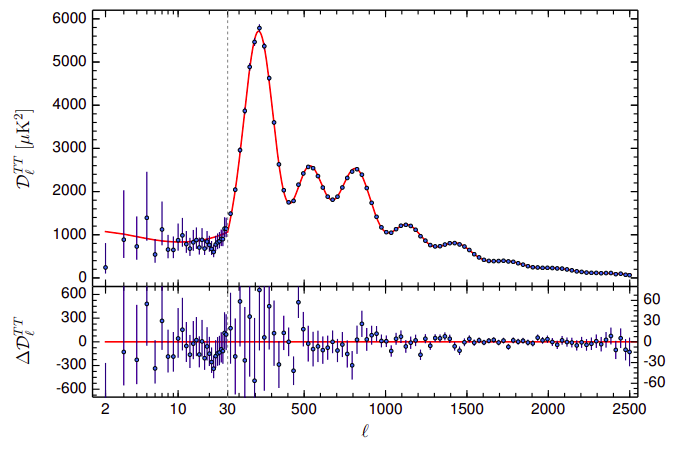
\includegraphics[width=5cm, height=3.5cm]{figs/PlanckSpectrum.png}
\end{center}
\end{figure}
\end{column}
\end{columns} \vfill

Other observations, such as the gravitational lensing effect, \textbf{also tend to further support the existence of dark matter} (cf. backup). \vfill
\end{frame}

\begin{frame}{Dark matter properties}
\justifying

\textbf{Several fundamental properties of dark matter} are nowadays known or assumed:

\begin{itemize}
\justifying
\item Dark matter \alert{is a particle}, given that it is assumed to have a certain mass;
\item It should be \alert{dark}, unable to interact with electromagnetic radation, otherwise we would have seen it already. It should then also be \textbf{electrically neutral};
\item It is \alert{non-baryonic}, because the energy density for the baryonic matter estimated from the CMB is too low to account for dark matter;
\item We only consider \alert{cold dark matter} since the widely accepted $\Lambda_{CDM}$ model is based on this assumption and this helps explaining the presence of large scale structures in the Universe;
\item It should \alert{have a mass in the electroweak scale}, between 10 GeV and 1 TeV, because of the relic density obtained from the thermal freeze-out mechanism \cite{Freezeout1}.
\item Finally, it should be \alert{long-lived}, since we expect them to have been produced during the Big Bang and they are still present in the Universe.
\end{itemize}

\end{frame}

\begin{frame}{Dark matter searches}
\justifying

\vspace{5pt}
\begin{block}{ \centering Weakly Interactive Massive Particles}\end{block} \vfill
The WIMPs are the dark matter candidates considered in this work, because of the so-called \textbf{WIMP miracle}. Indeed, they:

\begin{itemize}
\justifying
\item Are expected to interact very weakly with ordinary baryonic matter;
\item Have a mass in the 100 GeV-1 TeV range for reasonable electroweak production cross-section values;
\item Give us a dark matter while being able to solve the \textbf{hierarchy problem}.
\end{itemize} \vfill

\vspace{5pt}
\begin{block}{ \centering Main search strategies}\end{block} \vfill

\begin{columns}
	\begin{column}{0.45\textwidth}
\begin{figure}[htbp]
\begin{center}
\begin{figure}[htbp]
\begin{center}
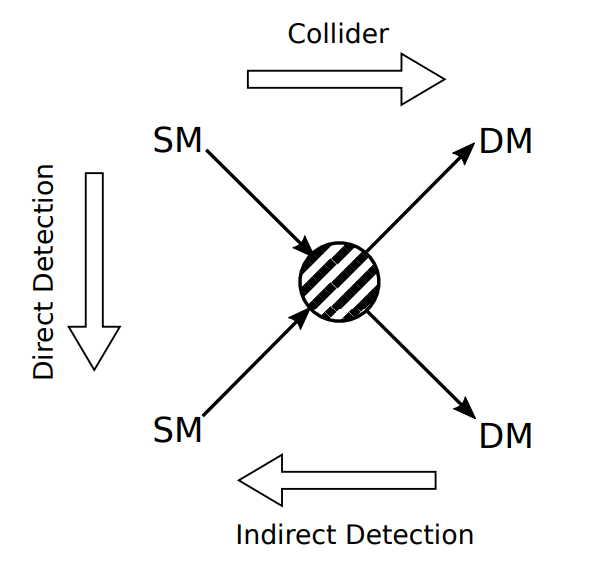
\includegraphics[width=4.2cm, height=3.5cm]{figs/ThreeWays.png}
\end{center}
\end{figure}
\end{center}
\end{figure}
\end{column}
\begin{column}{0.54\textwidth}
Different strategies are used:

\begin{itemize}
\justifying
\item The \alert{direct and indirect searches}, relying on the production of baryonic
matter from the interaction between two DM particles or on the observation of the interaction
between the dark and baryonic sectors;
\item And the \alert{collider production}, able to probe lower dark matter candidates masses.
\end{itemize}

\end{column}
\end{columns} \vfill
\end{frame}

\begin{frame}{Focus of this thesis I}
\justifying
We are searching for \alert{dark matter produced in association with either one or two top quarks}. Several \textbf{Simplified models} are considered:

\begin{itemize} 
	\justifying
	\item Spin 1/2 DM $\chi$ ($\in [1, 55]$ GeV, Dirac fermion) \\
	\item Spin 0 scalar (S)/pseudoscalar (PS) mediator $\phi$ (Yukawa-like structure of such interactions $\rightarrow$ gain from the coupling of the mediator to top quarks) \\
	\item Mediator mass $\in [10, 1000]$ GeV \\
	\item Coupling $g_{\chi}$ mediator/DM set to 1 (same for all $g_q$ couplings) \\
	%\item Most samples cross-section at NLO
	%\item No mixing between $\phi$ and the SM Higgs boson
\end{itemize}\vfill

\begin{columns}
	\begin{column}{0.675\textwidth}
		\begin{center}
			\begin{block}{ \centering $t/ \bar t$+DM tW models}\end{block}	
			%\alert{\textbf{$t$ + DM models}} \\ \vspace{5pt}
			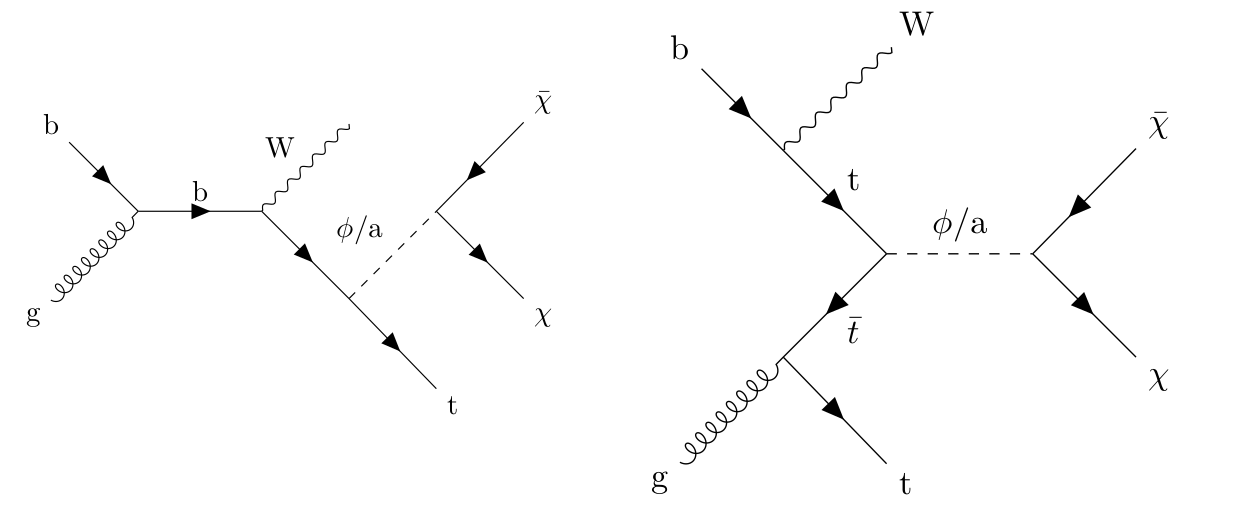
\includegraphics[width=1.0\textwidth]{figs/feynman_tDM_mine.png}
    		 \end{center}
	\end{column} \hfill
	\begin{column}{0.3\textwidth}
		\begin{center}
			\begin{block}{\centering $t \bar t$+DM model}\end{block}				
			%\alert{\textbf{$t \bar t$ + DM model}} \\ \vspace{5pt}
			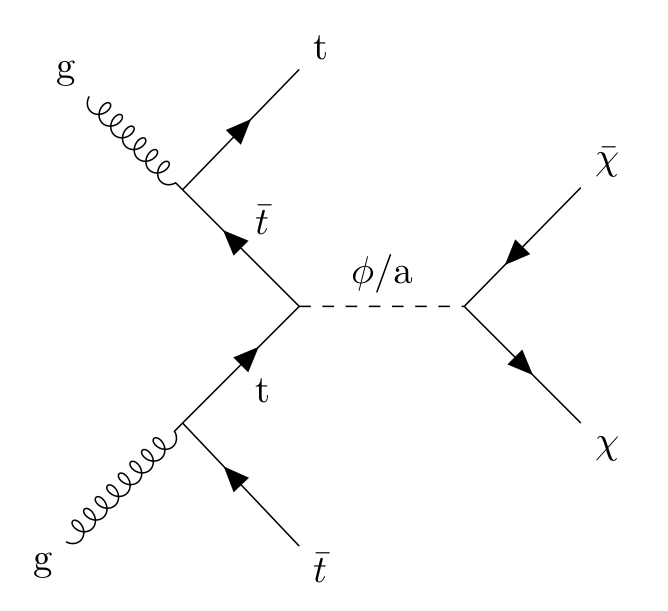
\includegraphics[width=1.0\textwidth]{figs/feynman_ttDM_mine.png}
    		 \end{center}
	\end{column} \hfill
\end{columns} \vfill

%The Yukawa coupling typically favors searches for dark matter \textbf{produced in association with heavy quarks} such as this one. Such MET+X are heavily depend on the MET spectrum, which is expected to be larger for the signals than most backgrounds. \vfill
\end{frame}

\begin{frame}{Focus of this thesis II}
\justifying
The \textbf{typical final state} of such models is made out of:
\begin{itemize}
\justifying
\item 1 or 2 b-tagged jets coming from the decay of the top quark(s);
\item 2 W bosons, seen as a combination of jets and leptons depending on the channel;
\item Some MET coming from the dark matter and the decay of the Ws;
\end{itemize} \vfill

In particular, we are studying the \alert{dilepton final state} in this work: 
\begin{itemize}
\justifying
\item Has the lowest branching ratio: BR($W \rightarrow l^+ + \nu_l) = (10.80 \pm 0.09)\%$ for each of the tree leptons (contains only $5\%$ of the signal events);
\item But, leptons can usually be reconstructed better than jets, resulting in lower systematic uncertainties;
\item And this channel also has the lowest number of backgrounds, resulting in a better signal isolation.
\end{itemize} \vfill

This channel is then \textbf{expected to be competitive with the hadronic channel}, especially when considering high mediator masses, which feature a higher global discrimination signal/background. \vfill
\end{frame}

\begin{frame}{Previous relevant results I}
\justifying
\vspace{5pt}
A similar analysis has already been published by CMS using 2016 data, considering the $t \bar t$+DM signal only and a combination of the three possible final states \cite{PreviousDoubleTopAllLep13CMS}. \vfill

\vspace{-10pt}
\begin{figure}[htbp]
\begin{center}
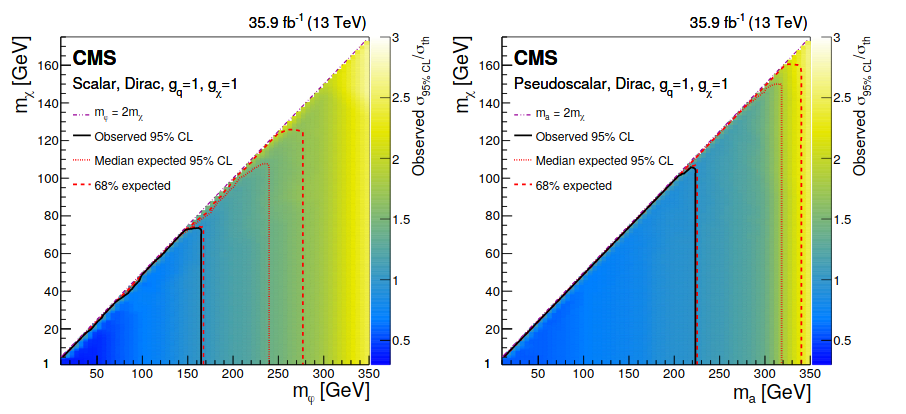
\includegraphics[width=11cm, height=4.8cm]{figs/CMSttbarExclusion.png}
\end{center}
\end{figure} \vfill

The observed (expected) limits \textbf{excluded a pseudoscalar mediator} with mass below 220 (320) GeV, and \textbf{a scalar mediator} with mass below 160 (240) GeV. \vfill
%This provided the \alert{most stringent constraints} ever obtained at the time on the scalar dark matter mediator model. \vfill
\end{frame}

\begin{frame}{Previous relevant results II}
\justifying
A \textbf{combination} of both the $t/ \bar t$+DM and $t \bar t$+DM processes has also been performed. \vfill
The inclusion of the single top signal process \alert{improved up to a factor 2} the limits obtained by the $t \bar t$ analysis on its own \cite{PreviousSingleDoubleTopAllLep13CMS}. This analysis:

\begin{itemize}
\item Only considered the 2016 data-taking period;
\item And only considered the semi-leptonic and hadronic final states.
\end{itemize} \vfill

\begin{center}
\begin{columns}
	\begin{column}{1.0\textwidth}
		\begin{center}
			%\begin{block}{\centering $t \bar t$+DM limits}\end{block}				
			%\alert{\textbf{$t \bar t$ + DM model}} \\ \vspace{5pt}
			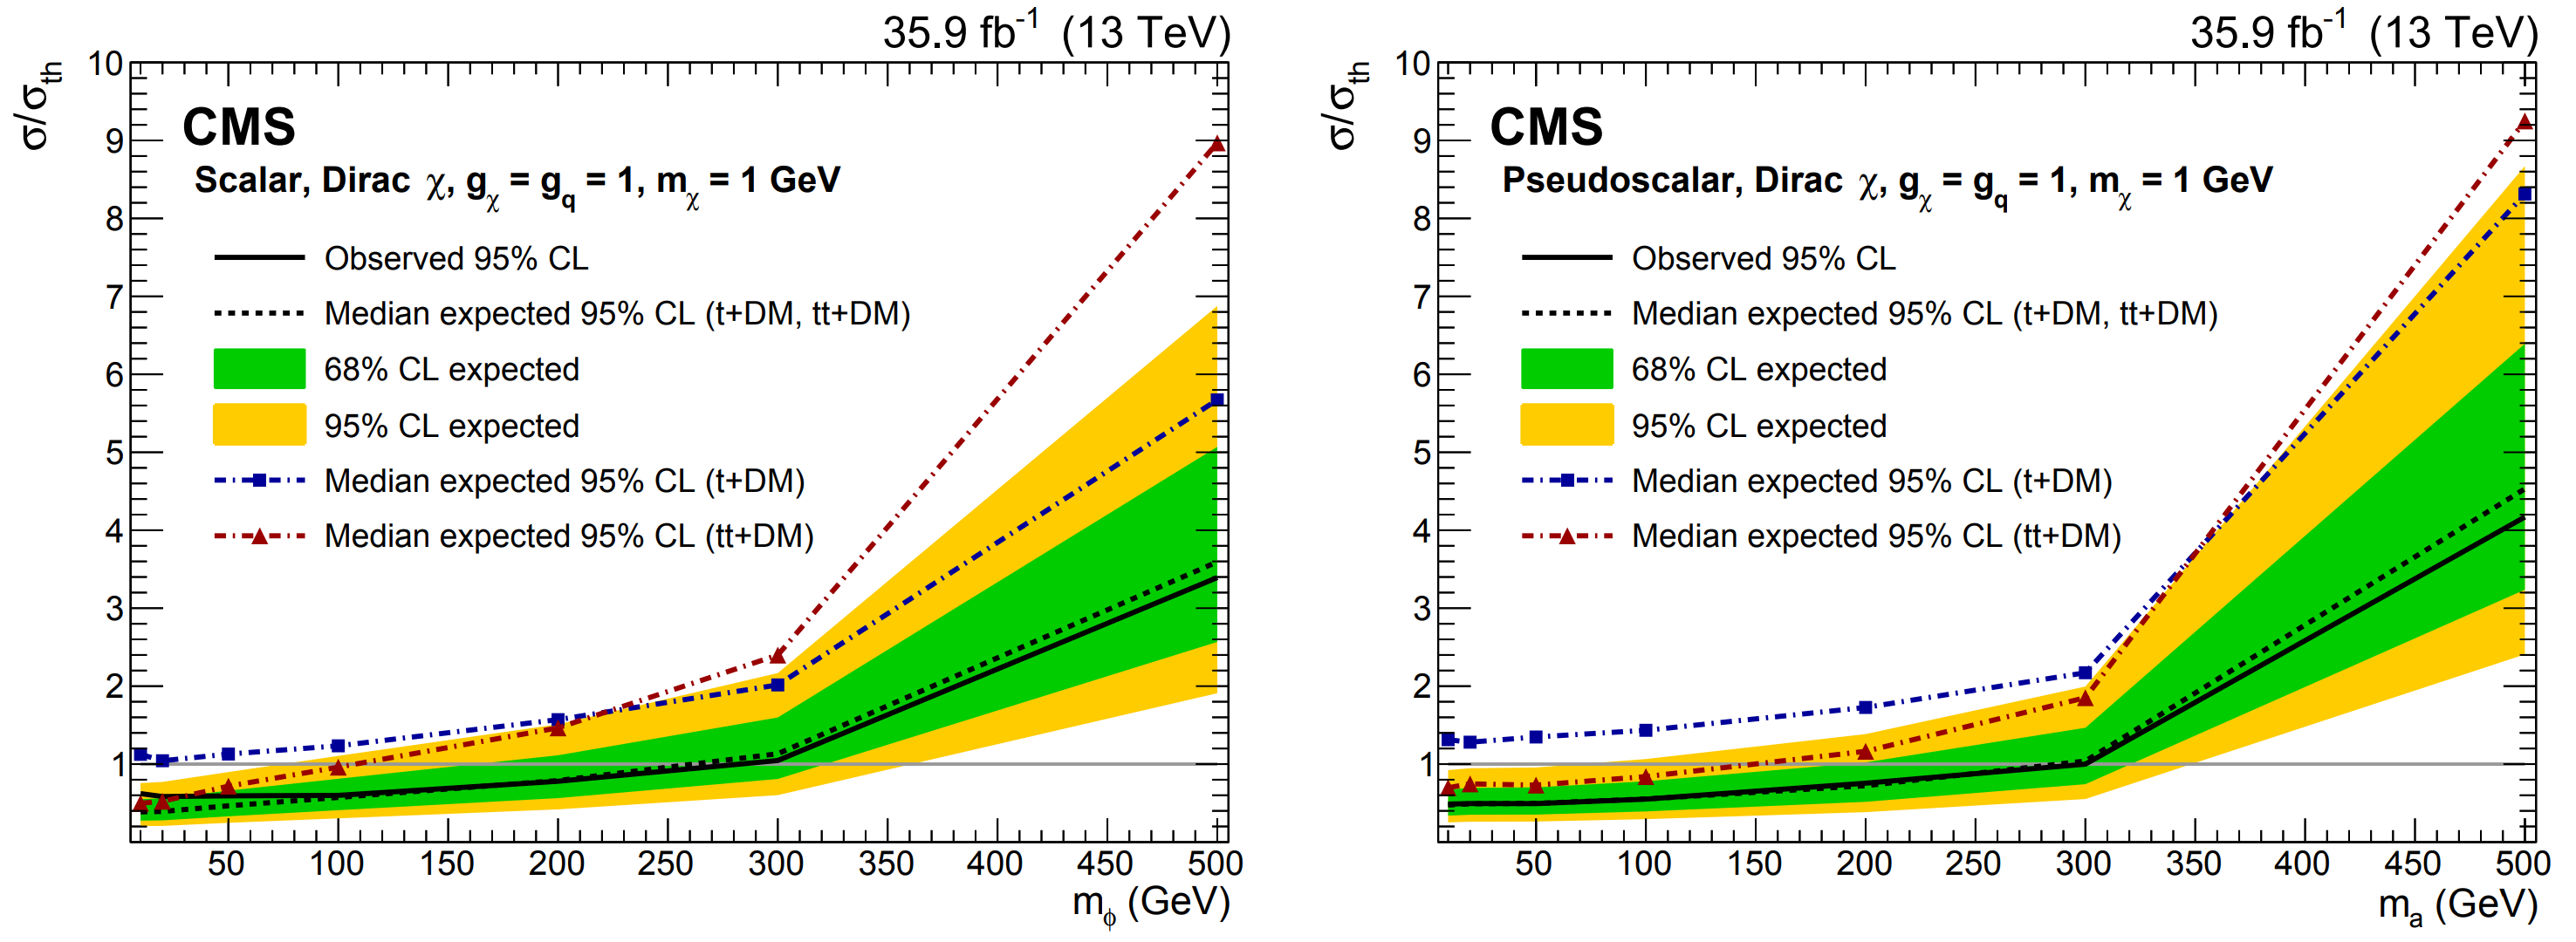
\includegraphics[width=1.0\textwidth]{figs/limitsprevious.png}
    		 \end{center}
	\end{column} \hfill
\end{columns}
\end{center} \vfill

Scalar (pseudoscalar) mediators were with this combination \alert{excluded up to 290 (300) GeV} at the 95\% confidence level. \vfill %The inclusion of the full Run II dataset and the dilepton final state \textbf{is expected to improve these results}.
\end{frame}










\begin{frame}[standout]
The experimental setup
\end{frame}

\begin{frame}{The Large Hadron Collider I}
\justifying
The data analyzed \alert{has been taken by the Large Hadron Collider}:

\begin{columns}
	\begin{column}{0.55	\textwidth}
	\begin{itemize}
\justifying
\item A 27km circular underground proton-proton collider, located at CERN;
\item Result of the collaboration of 22 countries;
\item Built in order to study and reproduce the conditions of the Universe at its origin;
\item Provided the collisions that lead to the discovery of the Higgs boson in 2012 \cite{HiggsDiscovery1, HiggsDiscovery2};
\item Currently the most powerful accelerator in the world with its center of mass energy $\sqrt{s} = 13$ TeV, therefore able to \textbf{scan new parts of the phase space}.
\end{itemize}
	\end{column}
	\begin{column}{0.48\textwidth}
	\begin{figure}[htbp]
\begin{center}
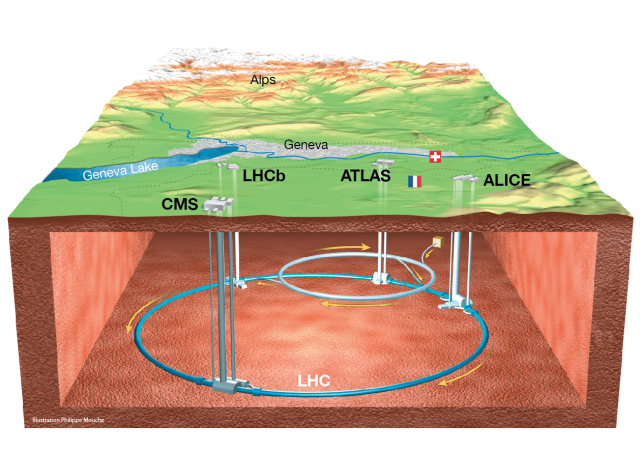
\includegraphics[width=5cm, height=3.6cm]{figs/LHCunderground.png}
\end{center}
\end{figure}
	\end{column}
\end{columns} \vfill

\vspace{10pt}
The data considered in this work has been collected during the \textbf{Run II of operation of the LHC} (from 2016 to 2018), at 13 TeV, totalling ($137.1 \pm 2.0$)~fb$^{-1}$ of data, selected by the different levels of trigger from the 40MhZ collision rate. \vfill
\end{frame} 

\begin{frame}{The Large Hadron Collider II}
\justifying
In the 4 interaction points of the LHC, \alert{4 detectors} have been placed: ATLAS, CMS, ALICE and LHCb, each having their own characteristics and features: \vfill

\begin{columns}
	\begin{column}{0.40	\textwidth}
\begin{center}
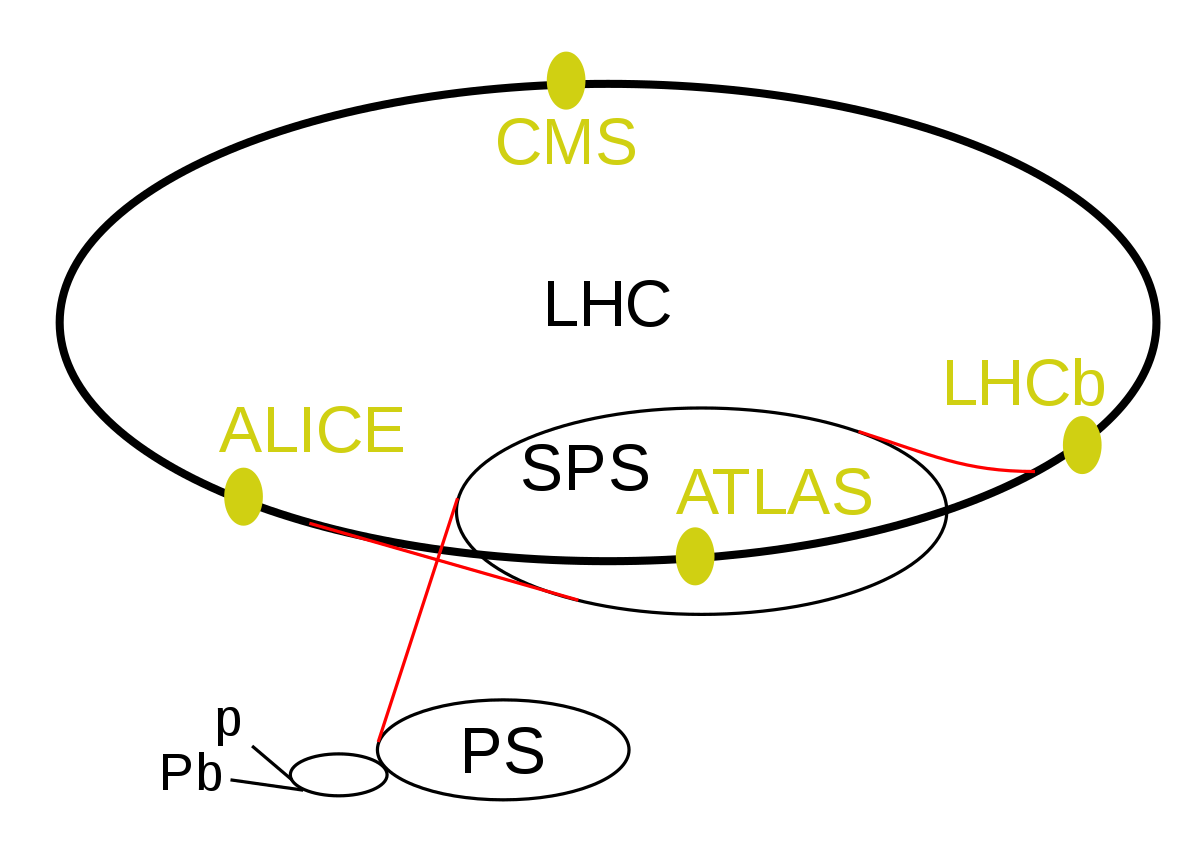
\includegraphics[width=5cm, height=3.6cm]{figs/LHCdetectors.png}
\end{center}
\end{column}
\begin{column}{0.58	\textwidth}
\begin{itemize}
\justifying
\item ATLAS and CMS are \textbf{general purpose detectors}, able to study exotic processes such as well as able to to make precision measurements on Standar Model physics;
\item ALICE is mostly dedicated to the study of the quark-gluon plasma originating from heavy ions collisions;
\item And LHCb has been designed to study the CP violation phenomena, which could be the sign of some new physics.
\end{itemize}
\end{column}
\end{columns} \vfill

\vspace{10pt}
The collisions analyzed in this work \alert{have been collected by the CMS detector}. \vfill
\end{frame}

\begin{frame}{The CMS detector I}
\justifying

\begin{columns}
\begin{column}{0.56	\textwidth}
\justifying
The \alert{Compact Muon Solenoid} is one of the two general purpose detectors of the LHC. Its main objectives consist in:
\begin{itemize}
\justifying
\item Searching for and studying the properties of the Higgs boson;
\item Trying to discover new BSM physics, such as the possible existence of dark matter.
\end{itemize}
\end{column}
\begin{column}{0.40	\textwidth}
\begin{center}
\includegraphics[width=4.7cm, height=3.5cm]{figs/CMSphoto.jpg}
\end{center}
\end{column}
\end{columns} \vfill

In a nutshell, CMS:
\begin{itemize}
\justifying
\item Is a relatively \textbf{compact} (14.000 tons, dsitributed over a 15m diameter and a length of 8m) cylindrical detector; 
\item Is made out of a central part with cylindrical shape, the barrel, and two endcaps, one on each side in order to be \textbf{as hermetic as possible}, covering all the possible angles around the beam pipe;
\item Has a \textbf{large solenoid} as middle piece, able to produce a 3.8T field;
\item Features a \textbf{powerful tracker and muon detection system}.
\end{itemize} \vfill
\end{frame}

\begin{frame}{The CMS detector II}
\justifying
The CMS detector is also \textbf{made out of different layers}, each having its own purpose, allowing for example to identify unequivocally each particle created. \vfill

\begin{figure}[htbp]
\begin{center}
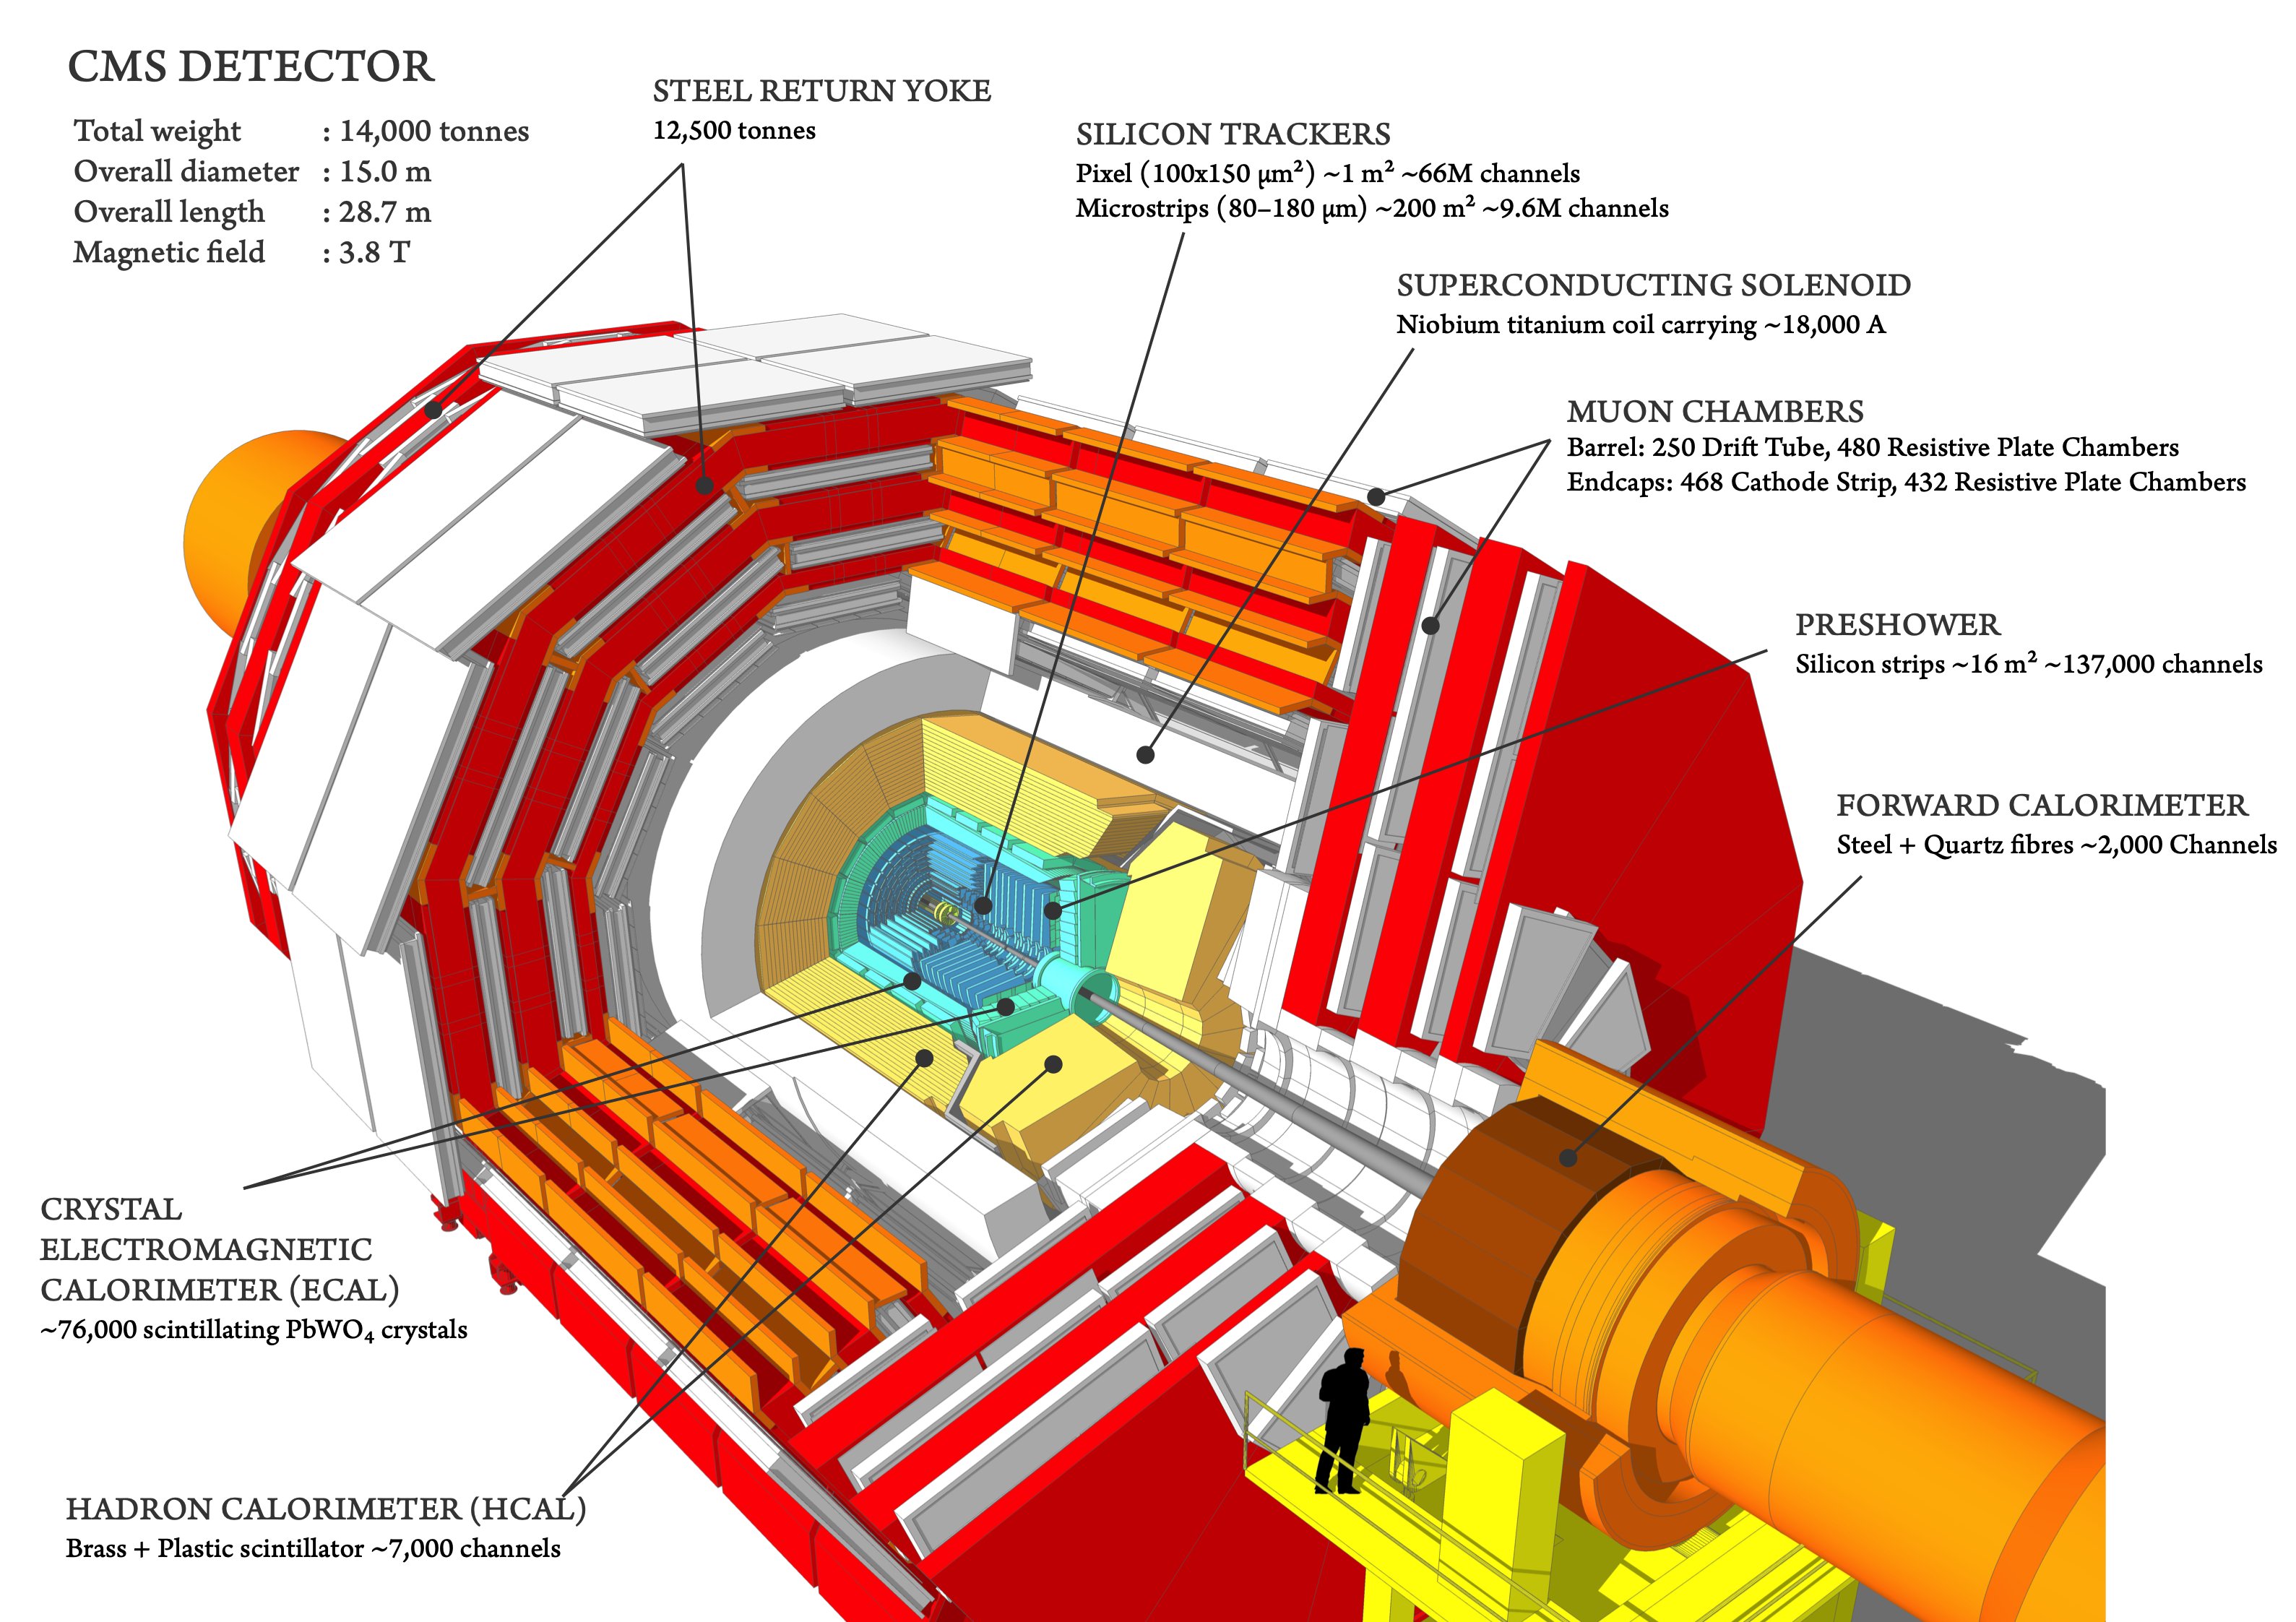
\includegraphics[width=9cm, height=6cm]{figs/CMS.png}
\end{center}
\end{figure} \vfill
\end{frame}

\begin{frame}{The CMS detector III}
\justifying
Each subdetector of CMS has been designed carefully to fill its specific purpose:

\begin{itemize}
\justifying
\item The \alert{tracker} is the innermost piece of CMS, able to reconstruct the trajectories of charged particles issued from the interaction vertices in a quick and precise way;
\item The \alert{Electromagnetic CALorimeter}, enclosing the tracker system and able to give information about the energy of electrons and photons;
\item The \alert{Hadronic CALorimater}, able to measure the energy of incident hadrons from the ionization process happening in its core;
\item The 12.5 meters long and 6 meters large \alert{solenoid}, allowing to measure precisely the charge and momentum of particles produced using the Lorentz effect, by measuring the curvature of their tracks;
\item And finally, the \alert{muon system}, covering more than 25 000 m$^2$ and made out of three different subsystems:

\begin{itemize}
\justifying
\item The \textbf{Drift Tubes} (DTs), in the barrel region;%, where the flux of muons is low and where the magnetic field is mostly uniform;
\item The \textbf{Cathode Strip Chambers} (CSCs) in the two endcaps;%, where the muon rates and background levels are much larger and where the magnetic field is large and non-uniform;
\item And the \textbf{Resistive Plate Chambers} (RPCs), mostly added to the barrel and to the endcap regions in order to cope with (in)ability of  the previous muon system to identify unequivocally the correct bunch crossing when the LHC is running at full luminosity.
\end{itemize}

\end{itemize}
\end{frame}













\begin{frame}[standout]
Global strategy
\end{frame}

\begin{frame}{Analysis strategy}
\justifying
Run II legacy paper being worked on, expected to \alert{combine both the $t$+DM and $t \bar t$+DM searches}, and the 3 possible final states (hadronic, semi-leptonic and dileptonic). \vfill

The effort is \alert{globally common} between the groups:
\begin{itemize}
\justifying
\item Objects will be defined in a common way
\item Control and signal region orthogonal between the channels
\begin{itemize}
\justifying
\item Number of leptons and b-jet categorization to improve the sensitivity by defining enriched single top/$t \bar t$ regions
\end{itemize}
\end{itemize}
\end{frame}






















\begin{frame}[standout]
Hadronic final state
\end{frame}

%\begin{frame}{Analysis strategy}
%\justifying
%
%\end{frame}

















\begin{frame}[standout]
Semi-leptonic final state
\end{frame}

%\begin{frame}{Analysis strategy}
%\justifying
%
%\end{frame}





















\begin{frame}[standout]
Dilepton final state
\end{frame}

\begin{frame}{Global strategy}
\justifying
The main idea is to train a MVA (either BDT or DNN) to \textbf{separate the two signals from the backgrounds}, mainly the SM $t \bar t$ and the single top. \vfill

\begin{block}{\centering Frameworks}\end{block}
\textbf{Two different frameworks} used in coordination, by IFCA and DESY:
\begin{itemize}
\justifying
\item Both using nanoAODv7 and the same background/signal samples;
\item Synchronization exercise performed in the different control and signal regions, in 2016, 2017 and 2018, as documented in our twiki \cite{ourTwiki}.
\end{itemize} \vfill
\end{frame}

\begin{frame}{Data and MC samples}
\justifying
\begin{block}{\centering Data}\end{block}
\alert{Single/double leptons datasets} built to avoid any eventual double counting, considering the 3 years of the Run II of operation of the LHC:
\begin{columns}
\hspace{15pt}
	\begin{column}{0.32\textwidth}
		\begin{itemize}
		\item ($35.9 \pm 0.9$) fb$^{-1}$
		\end{itemize}
	\end{column} \hfill
	\begin{column}{0.32\textwidth}
		\begin{itemize}
		\item ($41.5 \pm 1.0$)~fb$^{-1}$
		\end{itemize}
	\end{column} \hfill
	\begin{column}{0.32\textwidth}
		\begin{itemize}
		\item ($59.7 \pm 1.5$)~fb$^{-1}$
		\end{itemize}
	\end{column} \hfill
\end{columns} \vfill
\vspace{5pt}
A \textbf{blinding policy} is currently in place, allowing us to only look at $1$~fb$^{-1}$ of data per year near the signal regions. \vfill
\vspace{10pt}
\begin{block}{\centering Monte-Carlo}\end{block}
The \alert{major backgrounds} have been considered from MC and read from NanoAOD:

\begin{itemize}
\justifying
\item $t \bar t$: decaying to both 1 and 2 leptons;%, TuneCUETP8M2 (2016) and TuneCP5 (2017, 2018);
\item Single top: s, t and tW channels considered;
\item Drell-Yan: HT-binned samples to increase the statistics, with a correction factor derived from data applied;
\item TTZ and TTW: usually grouped together as TTV;
\item Others: dibosons, tribosons, non-prompt contamination (data-driven, not MC).
\end{itemize} \vfill
\end{frame}

\begin{frame}{DY Rin-out method}
\justifying
We want to \textbf{estimate the DY yields outside of the Z-peak from the data}:

\begin{itemize}
\justifying
\item Given the presence of large backgrounds (such as $t \bar t$) in the analysis region, we go inside of the Z-peak to compute the \alert{Rin-out factor}:
\begin{equation*}
N^{out}_{DY} = N^{in}_{DY, data} \cdot \left (\frac{N^{out}_{DY, MC}}{N^{in}_{DY, MC}} \right ) \equiv  N^{in}_{DY, data} \cdot R_{out/in,\text{ } MC}
\end{equation*}
\item To avoid any bias, the contamination of non-peaking backgrounds is removed and we additionally correct this factor by the ratio between the data/MC transfer factors in a CR close to the SR (asking for 0 b-jet instead of 1);
\item We then get this Rin-out in bins of MET and for each channel ($ee$, $\mu \mu$) separately:
\end{itemize}

\begin{figure}[htbp]
\begin{center}
\begin{minipage}[b]{.32\textwidth}
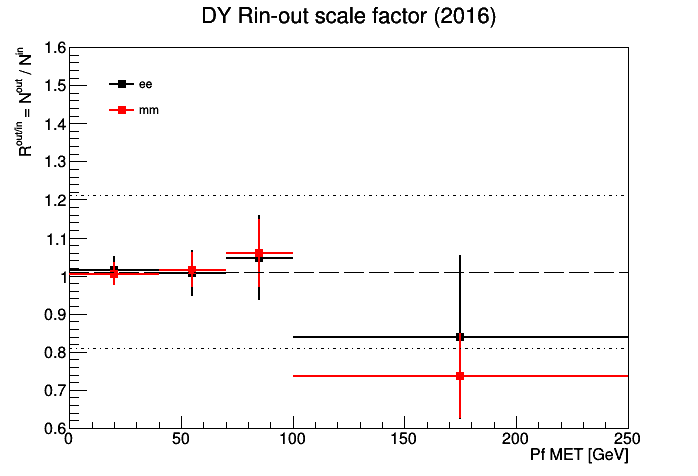
\includegraphics[width=4cm, height=3cm]{figs/Rinout2016.png}
\end{minipage} \hfill
\begin{minipage}[b]{.32\textwidth}
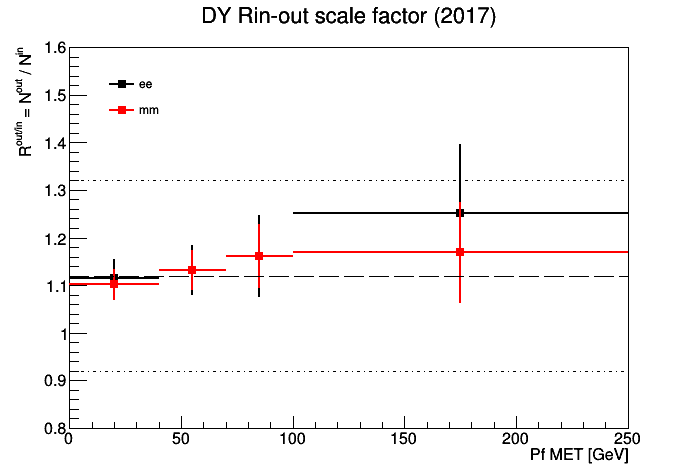
\includegraphics[width=4cm, height=3cm]{figs/Rinout2017.png}
\end{minipage} \hfill
\begin{minipage}[b]{.32\textwidth}
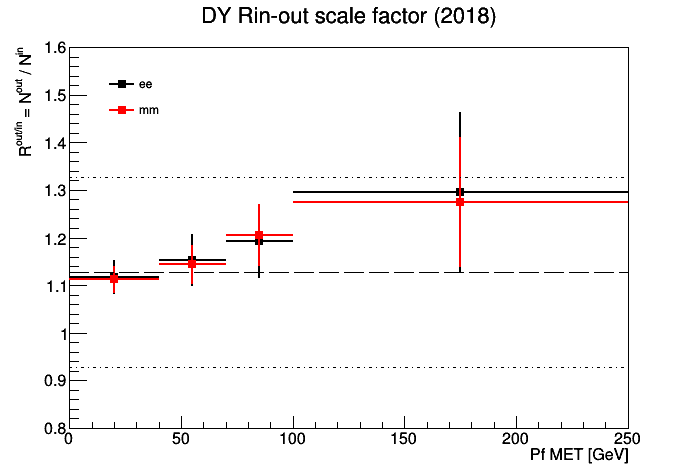
\includegraphics[width=4cm, height=3cm]{figs/Rinout2018.png}
\end{minipage} \hfill
\end{center}
\end{figure} \vfill

A flat scale factor and a fixed 20\% systematic uncertainty is then applied to the DY. \vfill
\end{frame}

\begin{frame}{Non-prompt contamination I}
\justifying
Fake leptons detection in the detector needs to be taken into account properly, through a \alert{data-driven tight-to-loose method} since the Monte-Carlo is not reliable in this case: \vfill

\begin{block}{\centering Fake rate}\end{block} \vspace{-5pt}
\begin{itemize}
\justifying
\item A QCD enriched region is defined with a looser particle selection criteria, where the misidentification should be high;
\item Any eventual contamination from electroweak processes in this region is removed;
\item The \alert{fake rate} is defined as the ratio between the fakeable object (lepton-like objects passing only the loose isolation requirements) and fully selected objects yields.
\end{itemize} \vfill

\begin{block}{\centering Prompt rate}\end{block} \vspace{-5pt}
\begin{itemize}
\justifying
\item The \textbf{prompt rate}, taking into account the real lepton contamination is calculated in a Z enriched region from a general tag and probe method.
\end{itemize} \vfill

Then, we calculate from data an extrapolation factor to go back to the signal region of the analysis and the results obtained are checked in a \alert{same sign control region}. \vfill
\end{frame}

\begin{frame}{Non-prompt contamination II}
\justifying
\begin{block}{\centering 2016 fake rate}\end{block}
\vspace{-15pt}
\begin{figure}[htbp]
\begin{center}
\begin{minipage}[b]{.49\textwidth}
\begin{block}{\centering Electron}\end{block}
\begin{center}
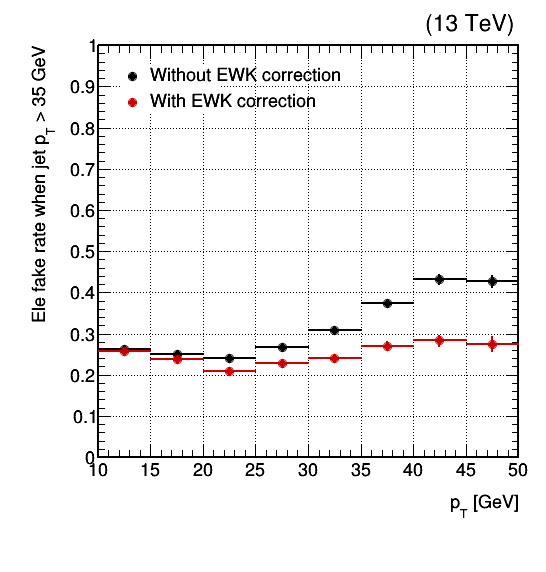
\includegraphics[width=4.2cm, height=3.7cm]{figs/Ele_FR_pt_35GeV_2016.png}
\end{center}
\end{minipage} \hfill
\begin{minipage}[b]{.49\textwidth}
\begin{block}{\centering Muon}\end{block}
\begin{center}
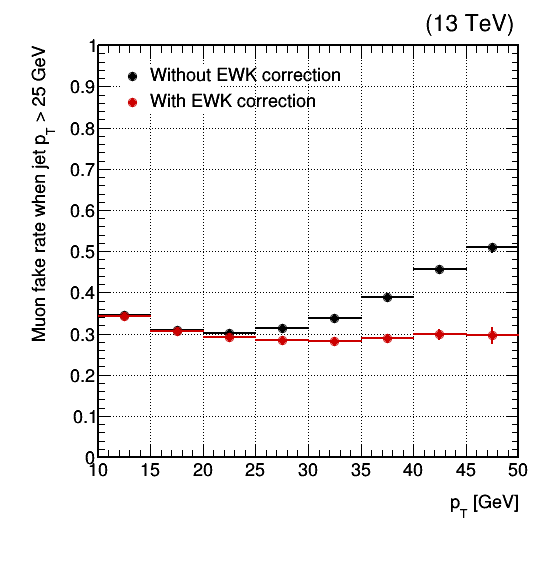
\includegraphics[width=4.2cm, height=3.7cm]{figs/Muon_FR_pt_25GeV_2016.png}
\end{center}
\end{minipage} \hfill
\end{center}
\end{figure} \vfill

\vspace{-10pt}
\begin{block}{\centering 2016 prompt rate}\end{block} \vspace{-10pt}
\begin{figure}[htbp]
\begin{center}
\begin{minipage}[b]{.49\textwidth}
\begin{center}
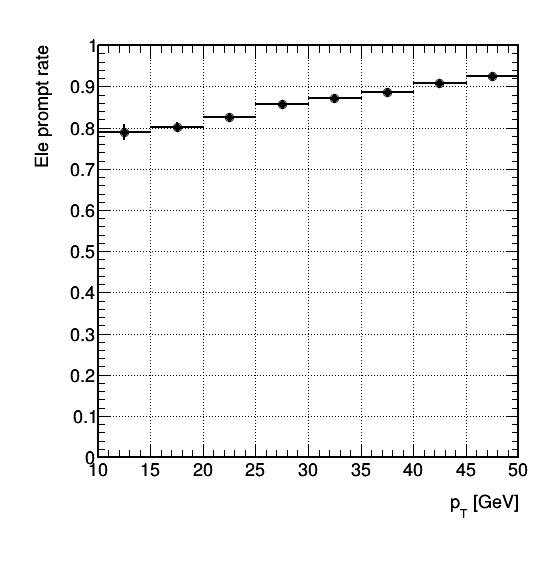
\includegraphics[width=4.2cm, height=3.7cm]{figs/Ele_PR_pt_2016.png}
\end{center}
\end{minipage} \hfill
\begin{minipage}[b]{.49\textwidth}
\begin{center}
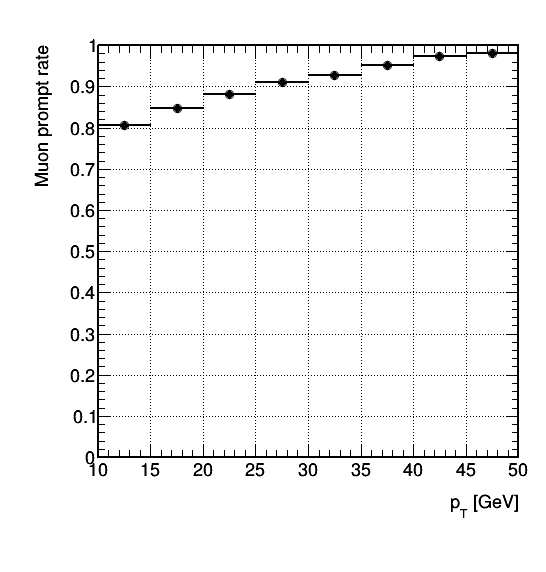
\includegraphics[width=4.2cm, height=3.7cm]{figs/Muon_PR_pt_2016.png}
\end{center}
\end{minipage} \hfill
\end{center}
\end{figure} \vfill

A \textbf{flat 30\% systematic uncertainty} is finally associated to this background in order to cover the statistical uncertainty plus eventual discrepancies in this control region. \vfill
\end{frame}

\begin{frame}{$t/\bar t+DM$ signal samples}
\justifying
\begin{block}{\centering Scalar mediators}\end{block} \vspace{-10pt}
\begin{figure}[htbp]
\centering
\begin{minipage}[b]{.49\textwidth}
\vspace{-5pt}
\begin{block}{\centering With normalization}\end{block}
\begin{center}
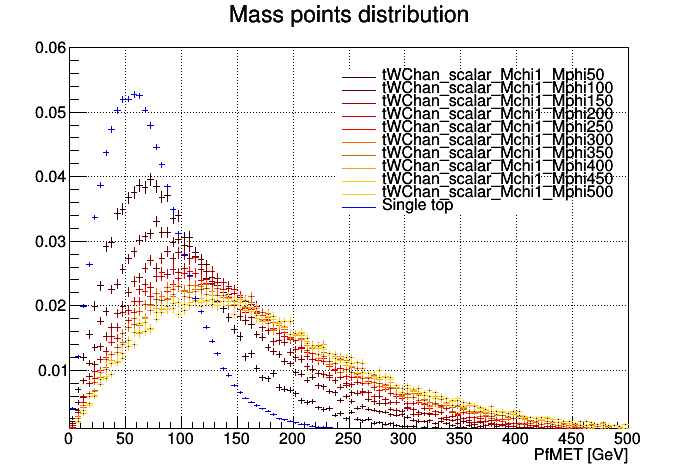
\includegraphics[width=5.2cm, height=3.5cm]{figs/singleTopScalarMETNorm.png}
\end{center}
\end{minipage}
\begin{minipage}[b]{.02\textwidth}\end{minipage}
\begin{minipage}[b]{.49\textwidth}
\vspace{-5pt}
\begin{block}{\centering Without normalization}\end{block}
\begin{center}
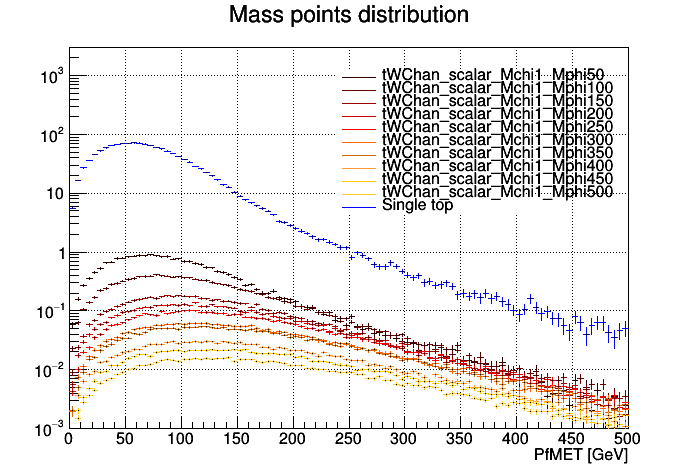
\includegraphics[width=5.2cm, height=3.5cm]{figs/singleTopScalarMET.png}
\end{center}
\end{minipage}
\end{figure} \vfill

\vspace{-5pt}
\begin{block}{\centering Pseudoscalar mediators}\end{block} \vspace{-10pt}
\begin{figure}[htbp]
\centering
\begin{minipage}[b]{.49\textwidth}
\begin{center}
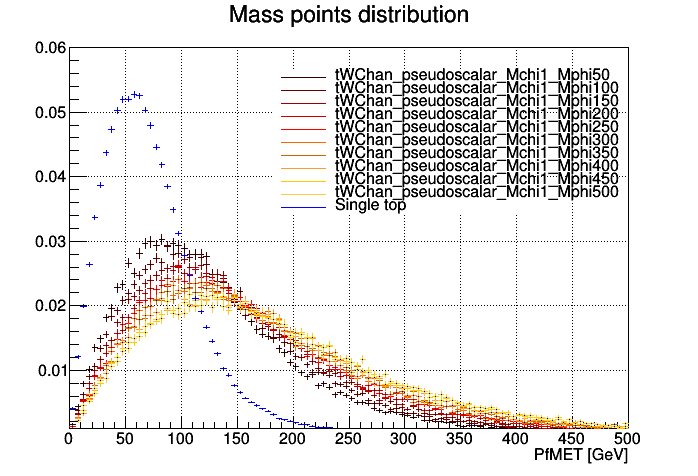
\includegraphics[width=5.2cm, height=3.5cm]{figs/singleTopPseudoMETNorm.png}
\end{center}
\end{minipage}\hfill
\begin{minipage}[b]{.49\textwidth}
\begin{center}
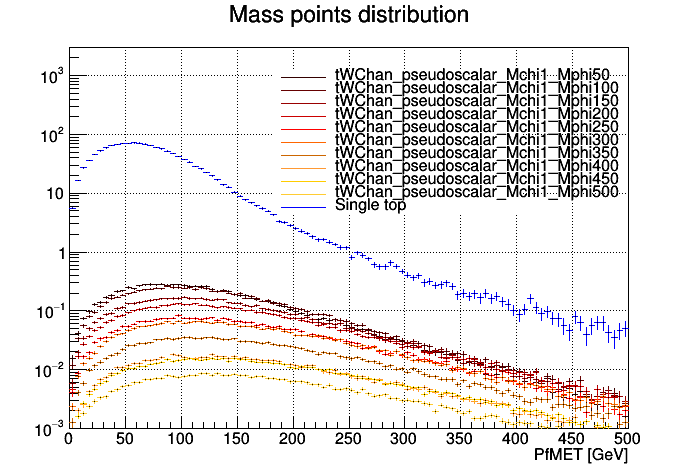
\includegraphics[width=5.2cm, height=3.5cm]{figs/singleTopPseudoMET.png}
\end{center}
\end{minipage} \hfill
\end{figure} \vfill
\end{frame}

\begin{frame}{$t \bar t+DM$ signal samples}
\justifying
\begin{block}{\centering Scalar mediators}\end{block} \vspace{-10pt}
\begin{figure}[htbp]
\centering
\begin{minipage}[b]{.49\textwidth}
\vspace{-5pt}
\begin{block}{\centering With normalization}\end{block}
\begin{center}
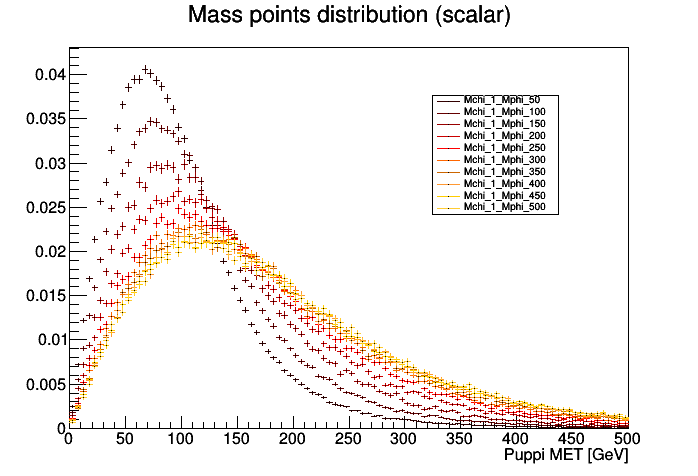
\includegraphics[width=5.2cm, height=3.5cm]{figs/scalarMETmChi1Norm.png}
\end{center}
\end{minipage}
\begin{minipage}[b]{.02\textwidth}\end{minipage}
\begin{minipage}[b]{.49\textwidth}
\vspace{-5pt}
\begin{block}{\centering Without normalization}\end{block}
\begin{center}
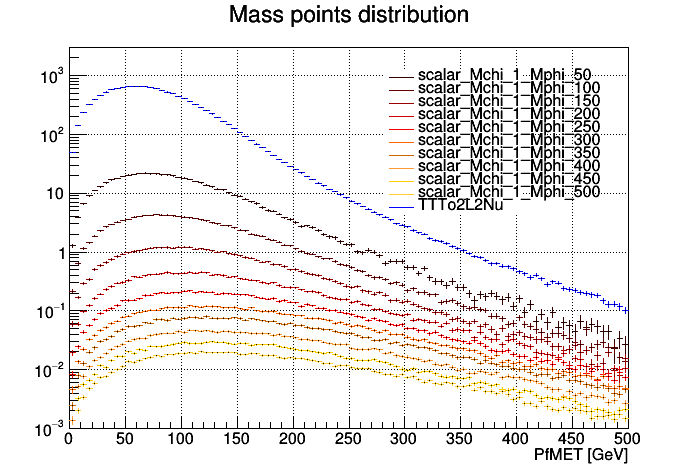
\includegraphics[width=5.2cm, height=3.5cm]{figs/scalarMETmChi1.png}
\end{center}
\end{minipage}
\end{figure} \vfill

\vspace{-5pt}
\begin{block}{\centering Pseudoscalar mediators}\end{block} \vspace{-10pt}
\begin{figure}[htbp]
\centering
\begin{minipage}[b]{.49\textwidth}
\begin{center}
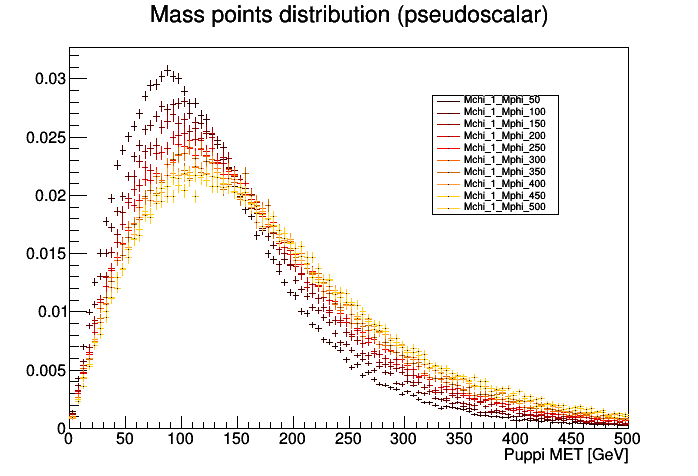
\includegraphics[width=5.2cm, height=3.5cm]{figs/pseudoscalarMETmChi1Norm.png}
\end{center}
\end{minipage}\hfill
\begin{minipage}[b]{.49\textwidth}
\begin{center}
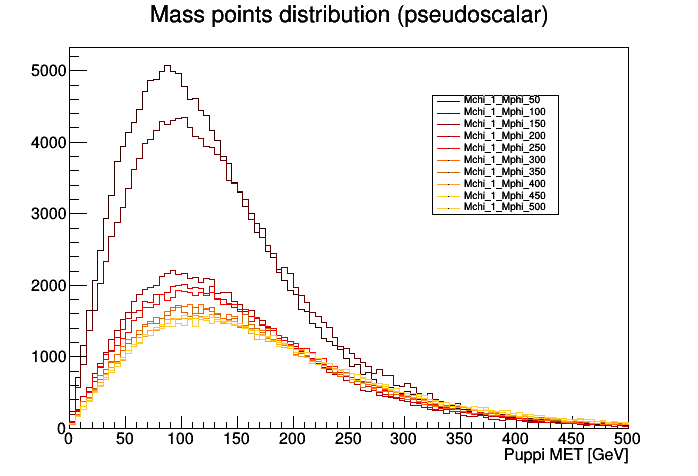
\includegraphics[width=5.2cm, height=3.5cm]{figs/pseudoscalarMETmChi1.png}
\end{center}
\end{minipage} \hfill
\end{figure} \vfill
\end{frame}

\begin{frame}{Objects definition}
\justifying

\end{frame}

\begin{frame}{Control regions}
\vspace{5pt}
\begin{block}{\centering Control regions}\end{block} \vfill
\vspace{-5pt}
\begin{itemize}
\item An \alert{inclusive} region:
\vspace{-10pt}
\begin{multicols}{2}
\begin{itemize}
\item Exactly 2 tight leptons ($p_T > 25, 20$ GeV)
\item Opposite sign leptons
\item $m_{ll} > 20$ GeV
\item At least 1 jet ($p_T > 30$ GeV, $|\eta| < 2.4$)
\item At least 1 deep CSV b-jet (medium WP)
\end{itemize}
\end{multicols} \vfill

\item A \alert{Drell-Yan} CR, defined as the inclusive region and:
\vspace{-10pt}
\begin{multicols}{2}
\begin{itemize}
\item 15 GeV Z window ($ee$/$\mu \mu$ channels)
\item $m_{T2}^{ll} > 80$ GeV
\end{itemize}
\end{multicols} \vfill

\item A \alert{$t \bar t$} CR, similar to the $t \bar t$ + DM signal region:
\begin{itemize}
\item But only for events classified as background by the MVA 
\item Currently blinded to 1fb$^{-1}$ per year
\end{itemize} \vfill \vspace{10pt}

\item A \alert{ttV} (ttW + ttZ) CR:
\vspace{-10pt}
\begin{multicols}{2}
\begin{itemize}
\item At least 3 tight leptons
\item $m_{T2}^{ll} > 80$ GeV
\end{itemize}
\end{multicols} \vfill

\item A \alert{same-sign CR} for the non-prompt background:
\vspace{-10pt}
\begin{multicols}{2}
\begin{itemize}
\item Inclusive with same sign leptons
\item 15 GeV Z-veto ($ee$/$\mu \mu$ channels)
\end{itemize}
\end{multicols} \vfill
\end{itemize}
\end{frame}

\begin{frame}{Conclusions}
\justifying

\end{frame}


\backupbegin

\begin{frame}[standout]
Back up
\end{frame}

\begin{frame}{Gravitational lensing}
\justifying
\vspace{5pt}
Consequence of the general relativity: massive objects placed between distant sources and the observer should be able to act as lenses and bend the light of the source. \vfill

\begin{itemize}
\justifying
\item The deviation of the light is proportional to the mass of the intermediate object, giving us a way to measure its mass;
\item The mass distribution obtained has been compared to the luminous distribution of several galaxies, leading to $8\sigma$ discrepancies \cite{BulletClusterSigma}.
\end{itemize} \vfill

\vspace{-5pt}
\begin{figure}[htbp]
\begin{center}
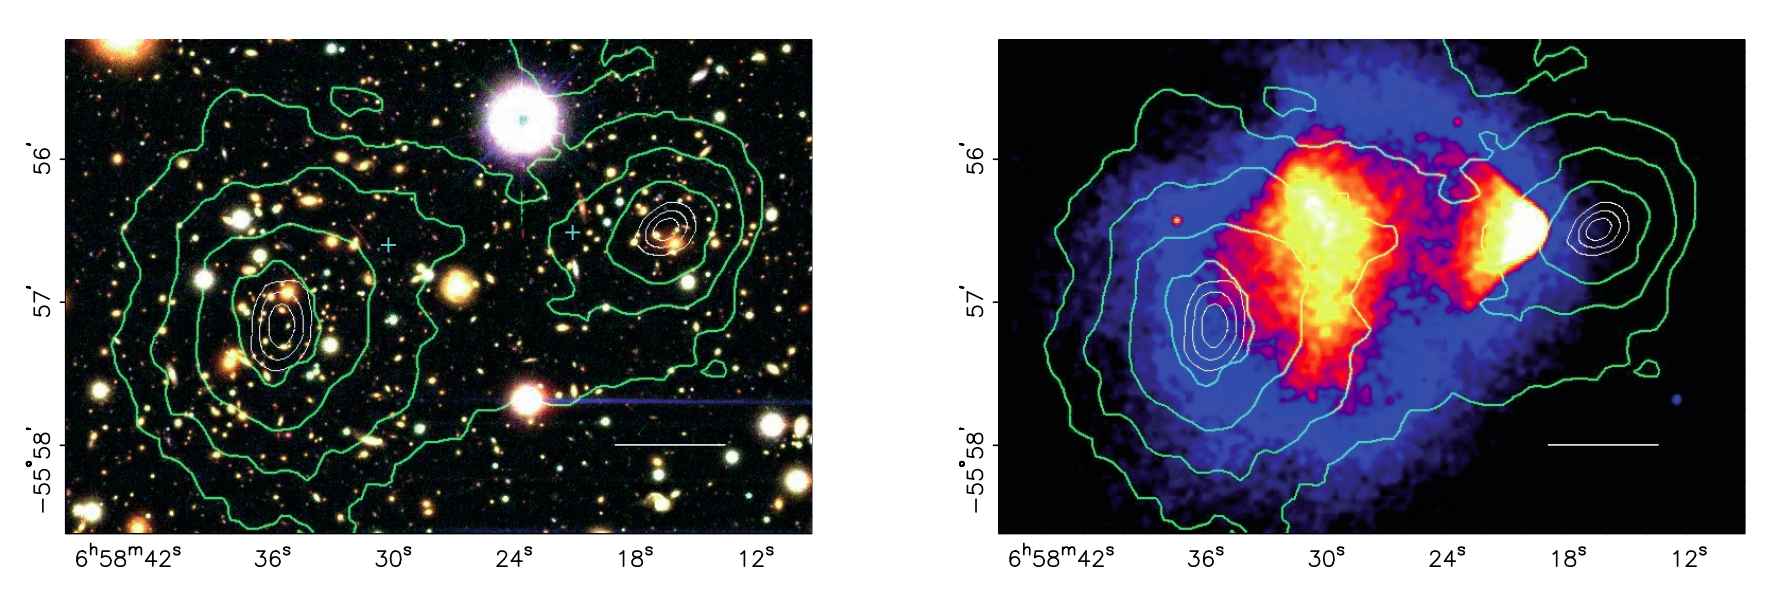
\includegraphics[width=11	cm, height=4cm]{figs/BulletCluster.png}
\end{center}
\end{figure} \vfill
\end{frame}

\begin{frame}{Thermal freeze-out}
\justifying
\vspace{5pt}
Schematic representation of the freeze-out process, representing the abundance of a
500 GeV dark matter with respect to the time and the impact of increasing cross-section annihilation
values on this freeze-out abundance. \vfill

\begin{figure}[htbp]
\begin{center}
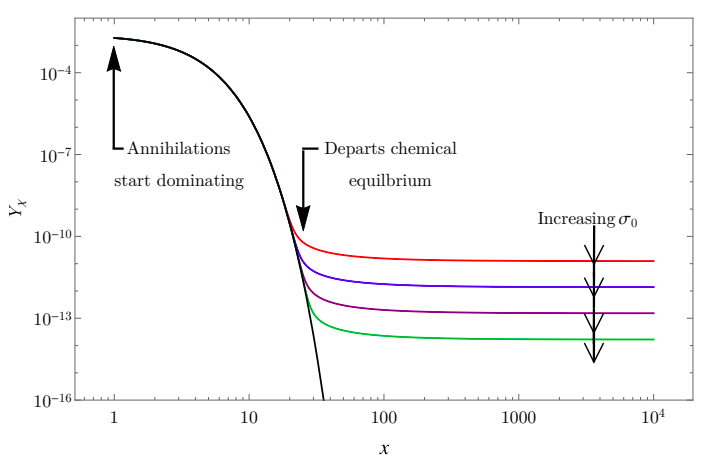
\includegraphics[width=9cm, height=6cm]{figs/FreezeOut.png}
\end{center}
\end{figure} \vfill
\end{frame}

\begin{frame}{Center of mass energy}
\justifying
The center of mass energy is defined as a Lorentz invariant quantity under any kind of boost resulting of the collisions between two protons (defined as $E_1, \overrightarrow{p_1}, m_1$ and $E_2, \overrightarrow{p_2}, m_2$) with a $\theta$ angle. \vfill

\begin{equation*}
\sqrt{s} = \sqrt{(m_1)^2 + (m_2)^2 + 2 \left (E_1 E_2-2 |\overrightarrow{p_1}| \text{ } |\overrightarrow{p_2}| \text{ cos}(\theta) \right )}
\end{equation*} \vfill

The LHC started its operation in 2008 running at an energy of 7 TeV, quickly moved to 8 TeV
and kept this level of energy during the end of the Run I of operation. In 2015, the energy was increased to 13 TeV. \vfill
An expected value of 14 TeV, the nominal energy for which the LHC was originally built, is
expected to be reached in the near future. \vfill
\end{frame}

\begin{frame}{Luminosity}
\justifying
The luminosity gives an indication on the number of collisions per second given by the accelerator. Increasing it is crucial to collect as much data as possible, to be able to isolate processes
having a low production cross section. \vfill

\begin{columns}
	\begin{column}{0.4	\textwidth}
	\justifying	
The rate of production $R$ of any given process can be expressed from the instantaneous luminosity $\mathcal{L}(t)$ and the process production cross-section $\sigma$:	
	
\begin{equation*}
\begin{dcases}
R = \mathcal{L} \cdot \sigma \\
N(T) = \sigma \int_0^T \mathcal{L}(t) dt = \sigma L
\end{dcases}
\end{equation*}
\end{column}
\begin{column}{0.6	\textwidth}
\begin{figure}[htbp]
\begin{center}
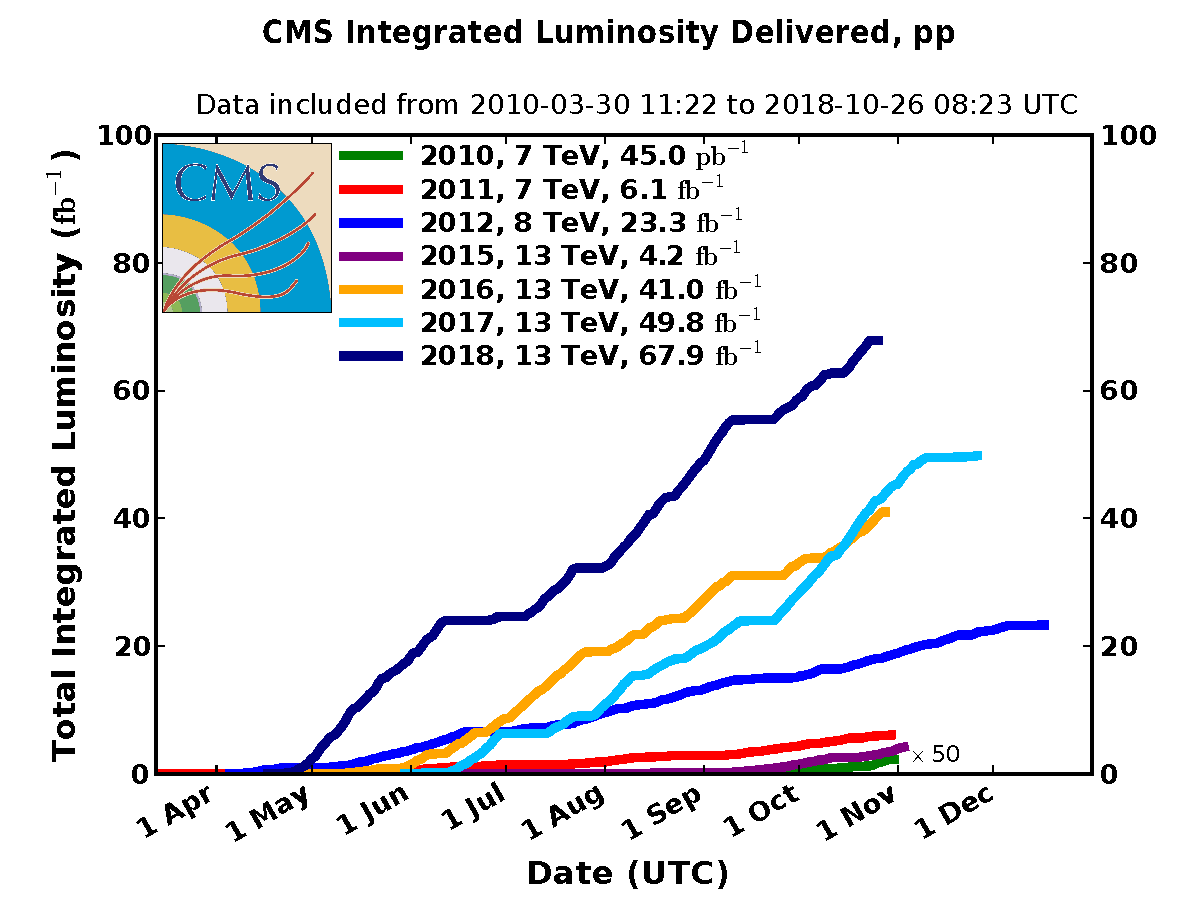
\includegraphics[width=7cm, height=5cm]{figs/CumuLumi.pdf}
\end{center}
\end{figure}
\end{column}
\end{columns}

\end{frame}

\begin{frame}{Pile-up}
\justifying
\vspace{5pt}
Because of the high density of protons within the beams, a bunch crossing in an experiment produces around 30-35 proton collisions. \vfill

\begin{figure}[htbp]
\begin{center}
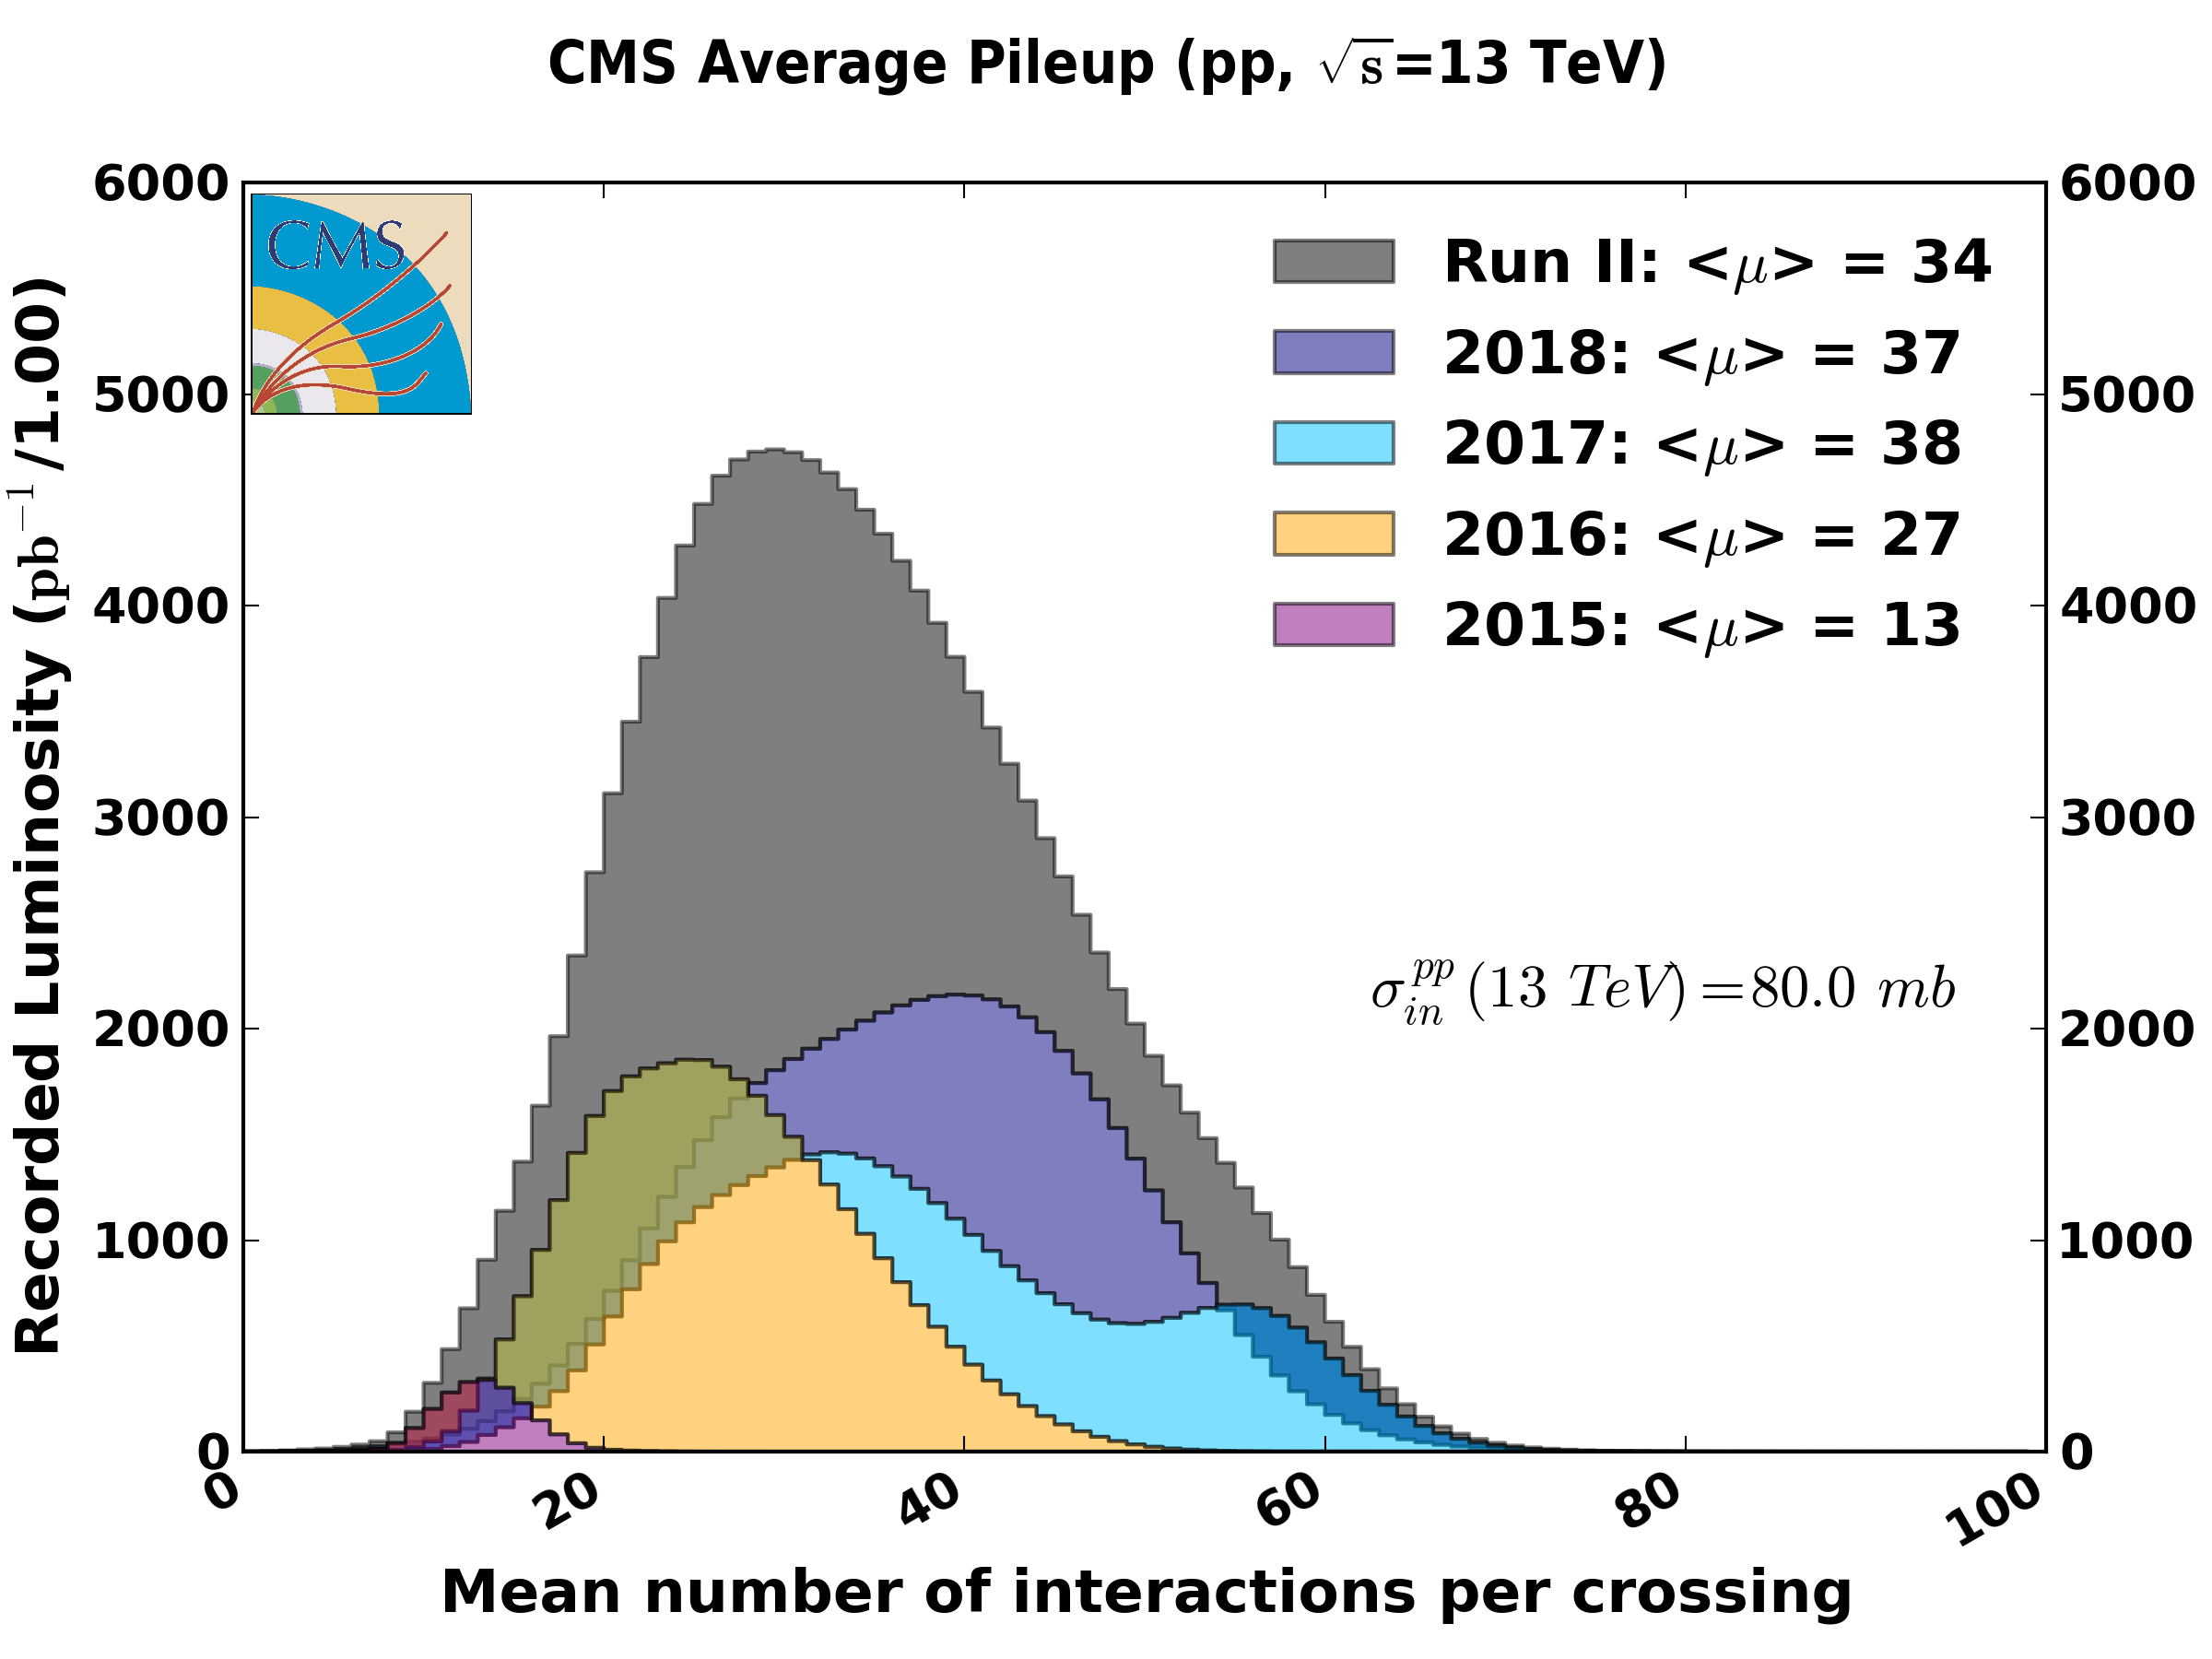
\includegraphics[width=8cm, height=5.5cm]{figs/PUSummary.png}
\end{center}
\end{figure} \vfill

The Primary Vertex is defined as the most interesting and energetic vertex, while the other vertices are usually referred to as the pile-up. \vfill
\end{frame}

\begin{frame}{LHC operational parameters}
\justifying
Key parameters of operation of the LHC, depending on the data-taking period:

\begin{table}
\begin{center}
\begin{tabular}{ c|c|c|c|c } 
 \hline
 Parameter & Run I & Run II & Run III & Design \\
\hline
Energy [TeV] & 7 $\rightarrow$ 8 & 13 & 13 & 14 \\
Bunch spacing [ns] & 50 & 25 & 25 & 25 \\
Intensity [$10^{11}$ protons per beam] & 1.6 & 1.2 & Up to 1.8 & 1.15 \\
Bunches & 1400 & 2500 & 2800 & 2800 \\
Emittance [$\mu m$] & 2.2 & 2.2 & 2.5 & 3.5 \\
$\beta^*$ [cm] & 80 & 30 $\rightarrow$ 25 & 30 $\rightarrow$ 25 & 55 \\
Crossing angle [$\mu$rad] & - & 300 $\rightarrow$ 260 & 300 $\rightarrow$ 260 & 285 \\
Peak luminosity [$10^{34}$ cm$^{-2}$ s$^{-1}$] & 0.8 & 2.0 & 2.0 & 1.0 \\
Peak pile-up & 45 & 60 & 55 & 25 \\
 \hline
\end{tabular}
\end{center}
\end{table}
\end{frame}

\begin{frame}{CMS tracker I}
\justifying
The tracker is the innermost piece of CMS, able to reconstruct the trajectories of charged particles issued from the interaction vertices in a quick and precise way:
\begin{itemize}
\justifying
\item Needs to be extremely fast to read the 40MhZ of collision data, while being resistant to the radiation (expected lifetime $\sim 10$ years);
\item It should be as small as possible to minize the interaction between the detector and the particles created;
\item However, fast electronics usually needs to be cooled down, which increases the size of the subdetector.
\end{itemize} \vfill

Made out of two main parts: 
\begin{itemize}
\justifying
\item The \alert{pixel detector}, made out 60 millions pixels which make up the 1856 after an modules of this detector, covering an area of $\sim 1$ m$^2$;
\item The \alert{silicon strip detector}, covering an area of $\sim 200$ m$^2$, and made out of three different sub-systems for hermeticity.
\end{itemize} \vfill

A charged particle crossing the tracker will leave a hit each time it crosses one of the silicon sensors, allowing us to reconstruct its track. \vfill
\end{frame}

\begin{frame}{CMS tracker II}
\justifying
\vspace{5pt}
The silicon detector is divided into three main parts:
\begin{itemize}
\item The Tracker Inner Barrel and Disks (TIB/TBD), using micro-strips parallel in the barrel and perpendicular to the beam axis in the endcaps;
\item The Tracker Outer Barrel (TOB), adding 6 measurement layers to the tracker;
\item And finally the Tracker EndCaps (TECs), made out of 9 disks, completing the system at high pseudorapidities.
\end{itemize} \vfill

\begin{figure}[htbp]
\begin{center}
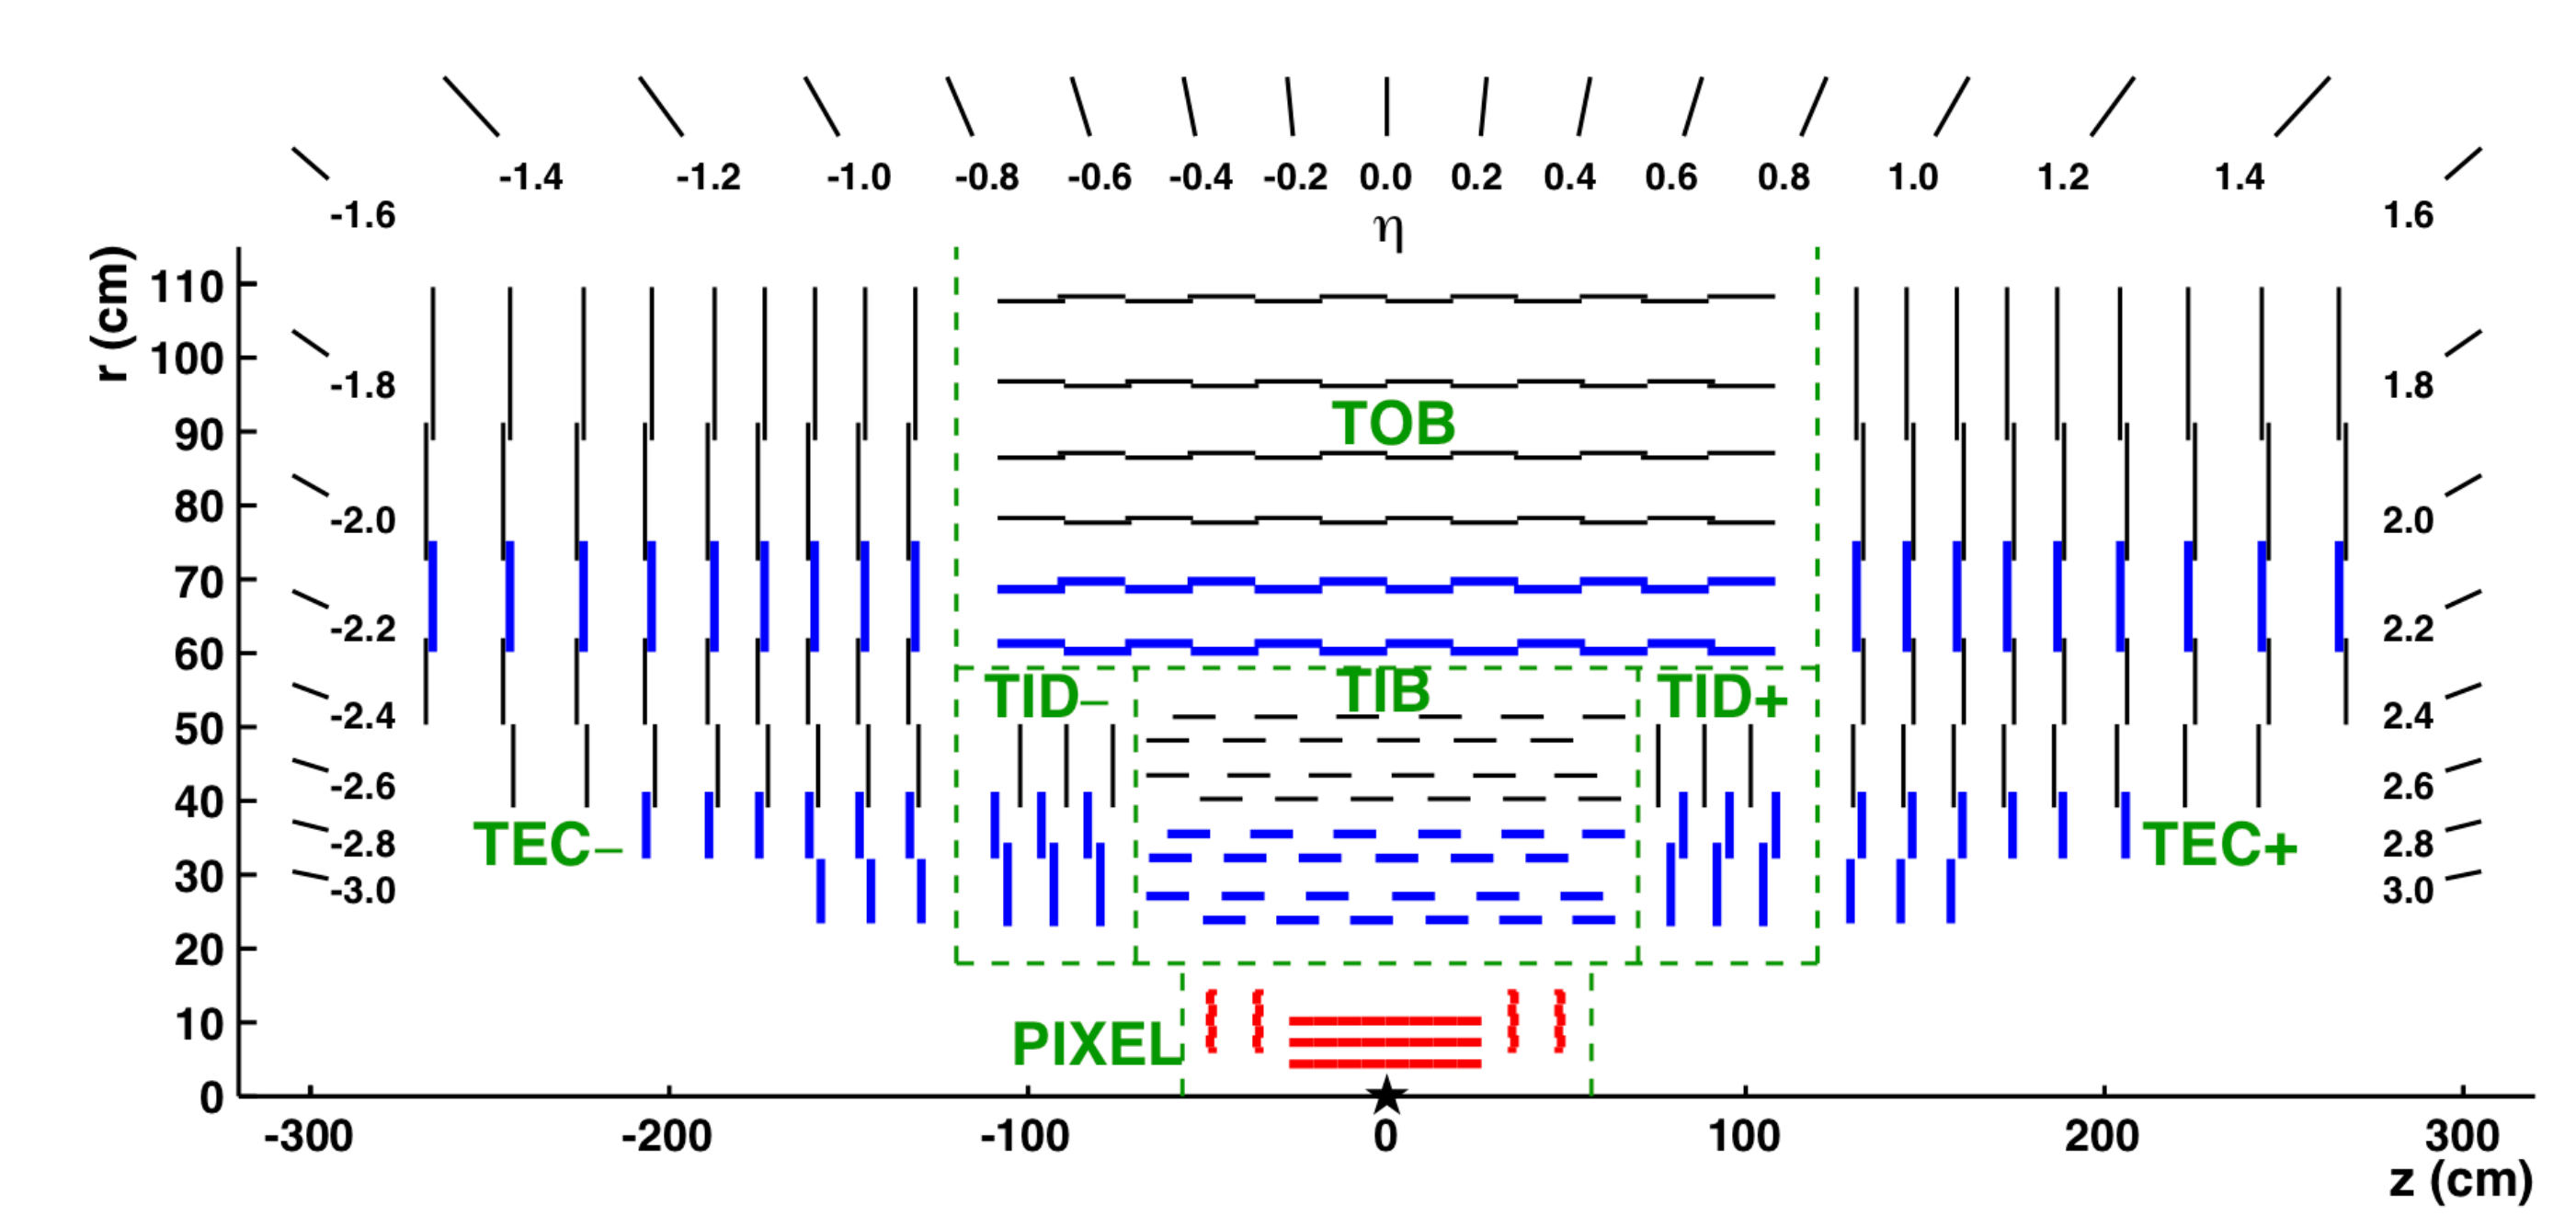
\includegraphics[width=10cm, height=5.2cm]{figs/CMSTracker.png}
\end{center}
\end{figure}\vfill
\end{frame}

\begin{frame}{CMS electromagnetic calorimeter I}
\justifying
\vspace{5pt}
The ECAL is a subdetector sitting inside the solenoid but enclosing the tracker
system that gives information about the energy of electrons and photons, both able to interact
electromagnetically with its crystals. \vfill

\begin{columns}
	\begin{column}{0.45 \textwidth}
	Made out of different layers:
	\begin{itemize}
	\justifying
	\item The barrel part (EB), at $|\eta| < 1.479$, made out of 61 200 lead tungstate (PbWO$_4$) crystals;
	\item Two endcaps, each made out of 7 324 crystals, increasing the coverage of the detector up to $|\eta| < 3$;
	\item The preshower, helping with the identification of electrons
against minimum ionizing particles.
	\end{itemize}
	\end{column}
	\begin{column}{0.55 \textwidth}
	\begin{figure}[htbp]
\begin{center}
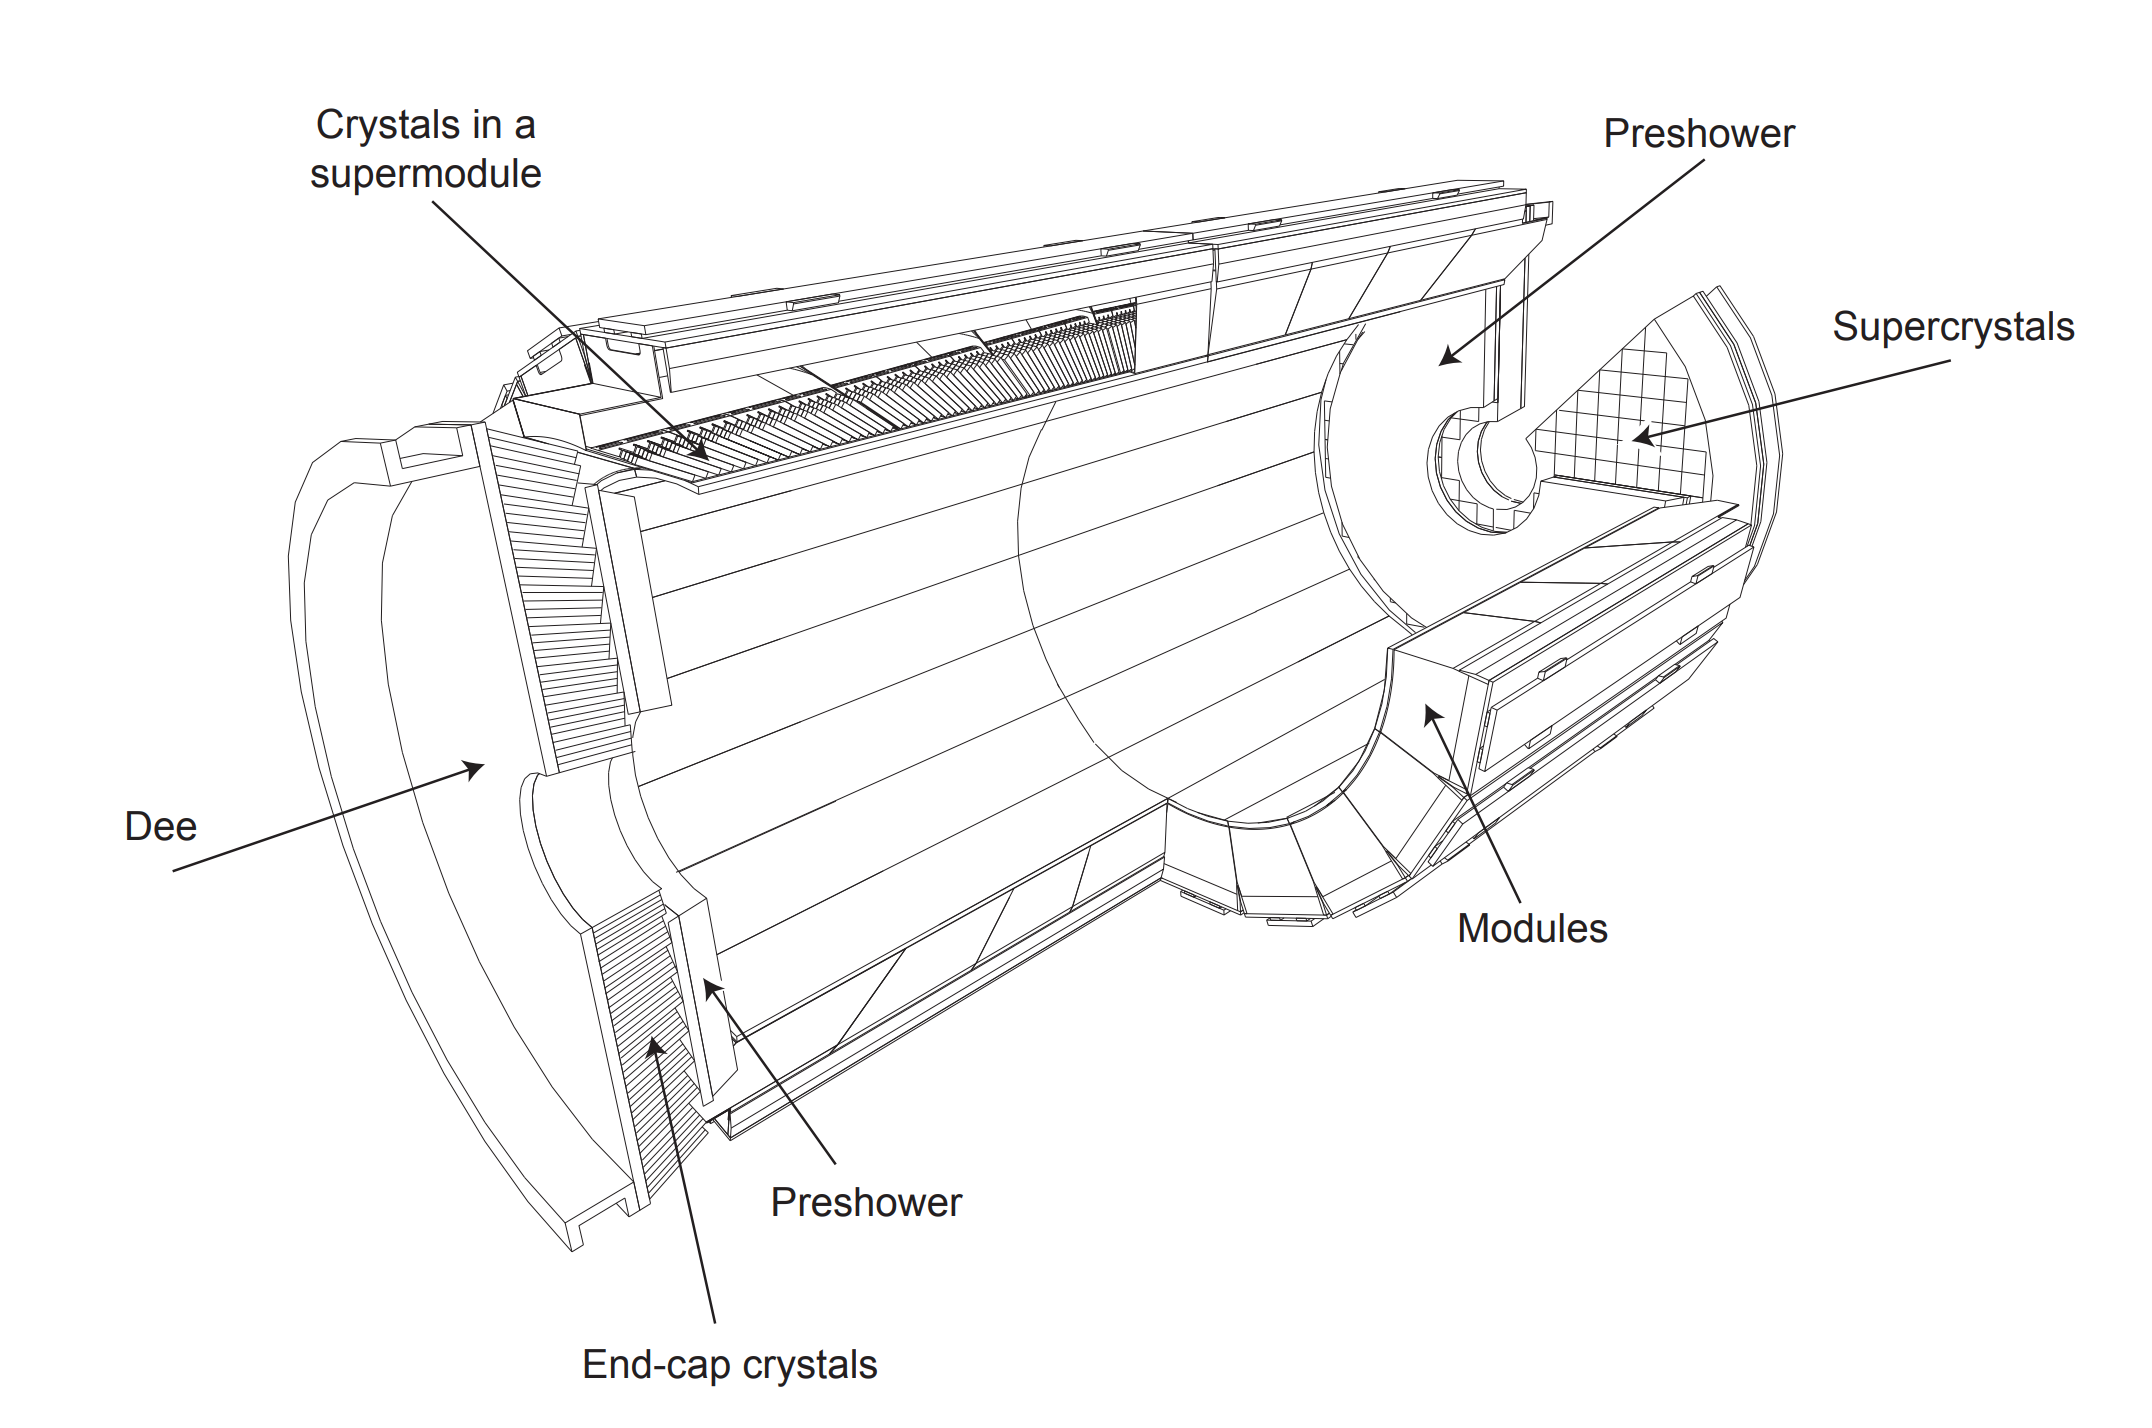
\includegraphics[width=6.6cm, height=4cm]{figs/CMSEcal.png}
\end{center}
\end{figure}
	\end{column}
\end{columns} \vfill

\end{frame}

\begin{frame}{CMS electromagnetic calorimeter II}
\justifying
\vspace{10pt}
The principle of action of the ECAL is simple, and is based on \alert{electromagnetic showers}. When an electron or a photon enters the ECAL, it starts to interact in different ways:
\begin{itemize}
\item Photons will mainly produce pairs of electrons and anti-electrons;
\item Electrons themselves tend to emit additional photons by bremsstrahlung effect.
\end{itemize}
This results in a chain reaction during which the incident particle gives most of its energy to the detector, energy measurable using photodetectors and photomultipliers. \vfill

\begin{columns}
	\begin{column}{0.45 \textwidth}
\begin{figure}[htbp]
\begin{center}
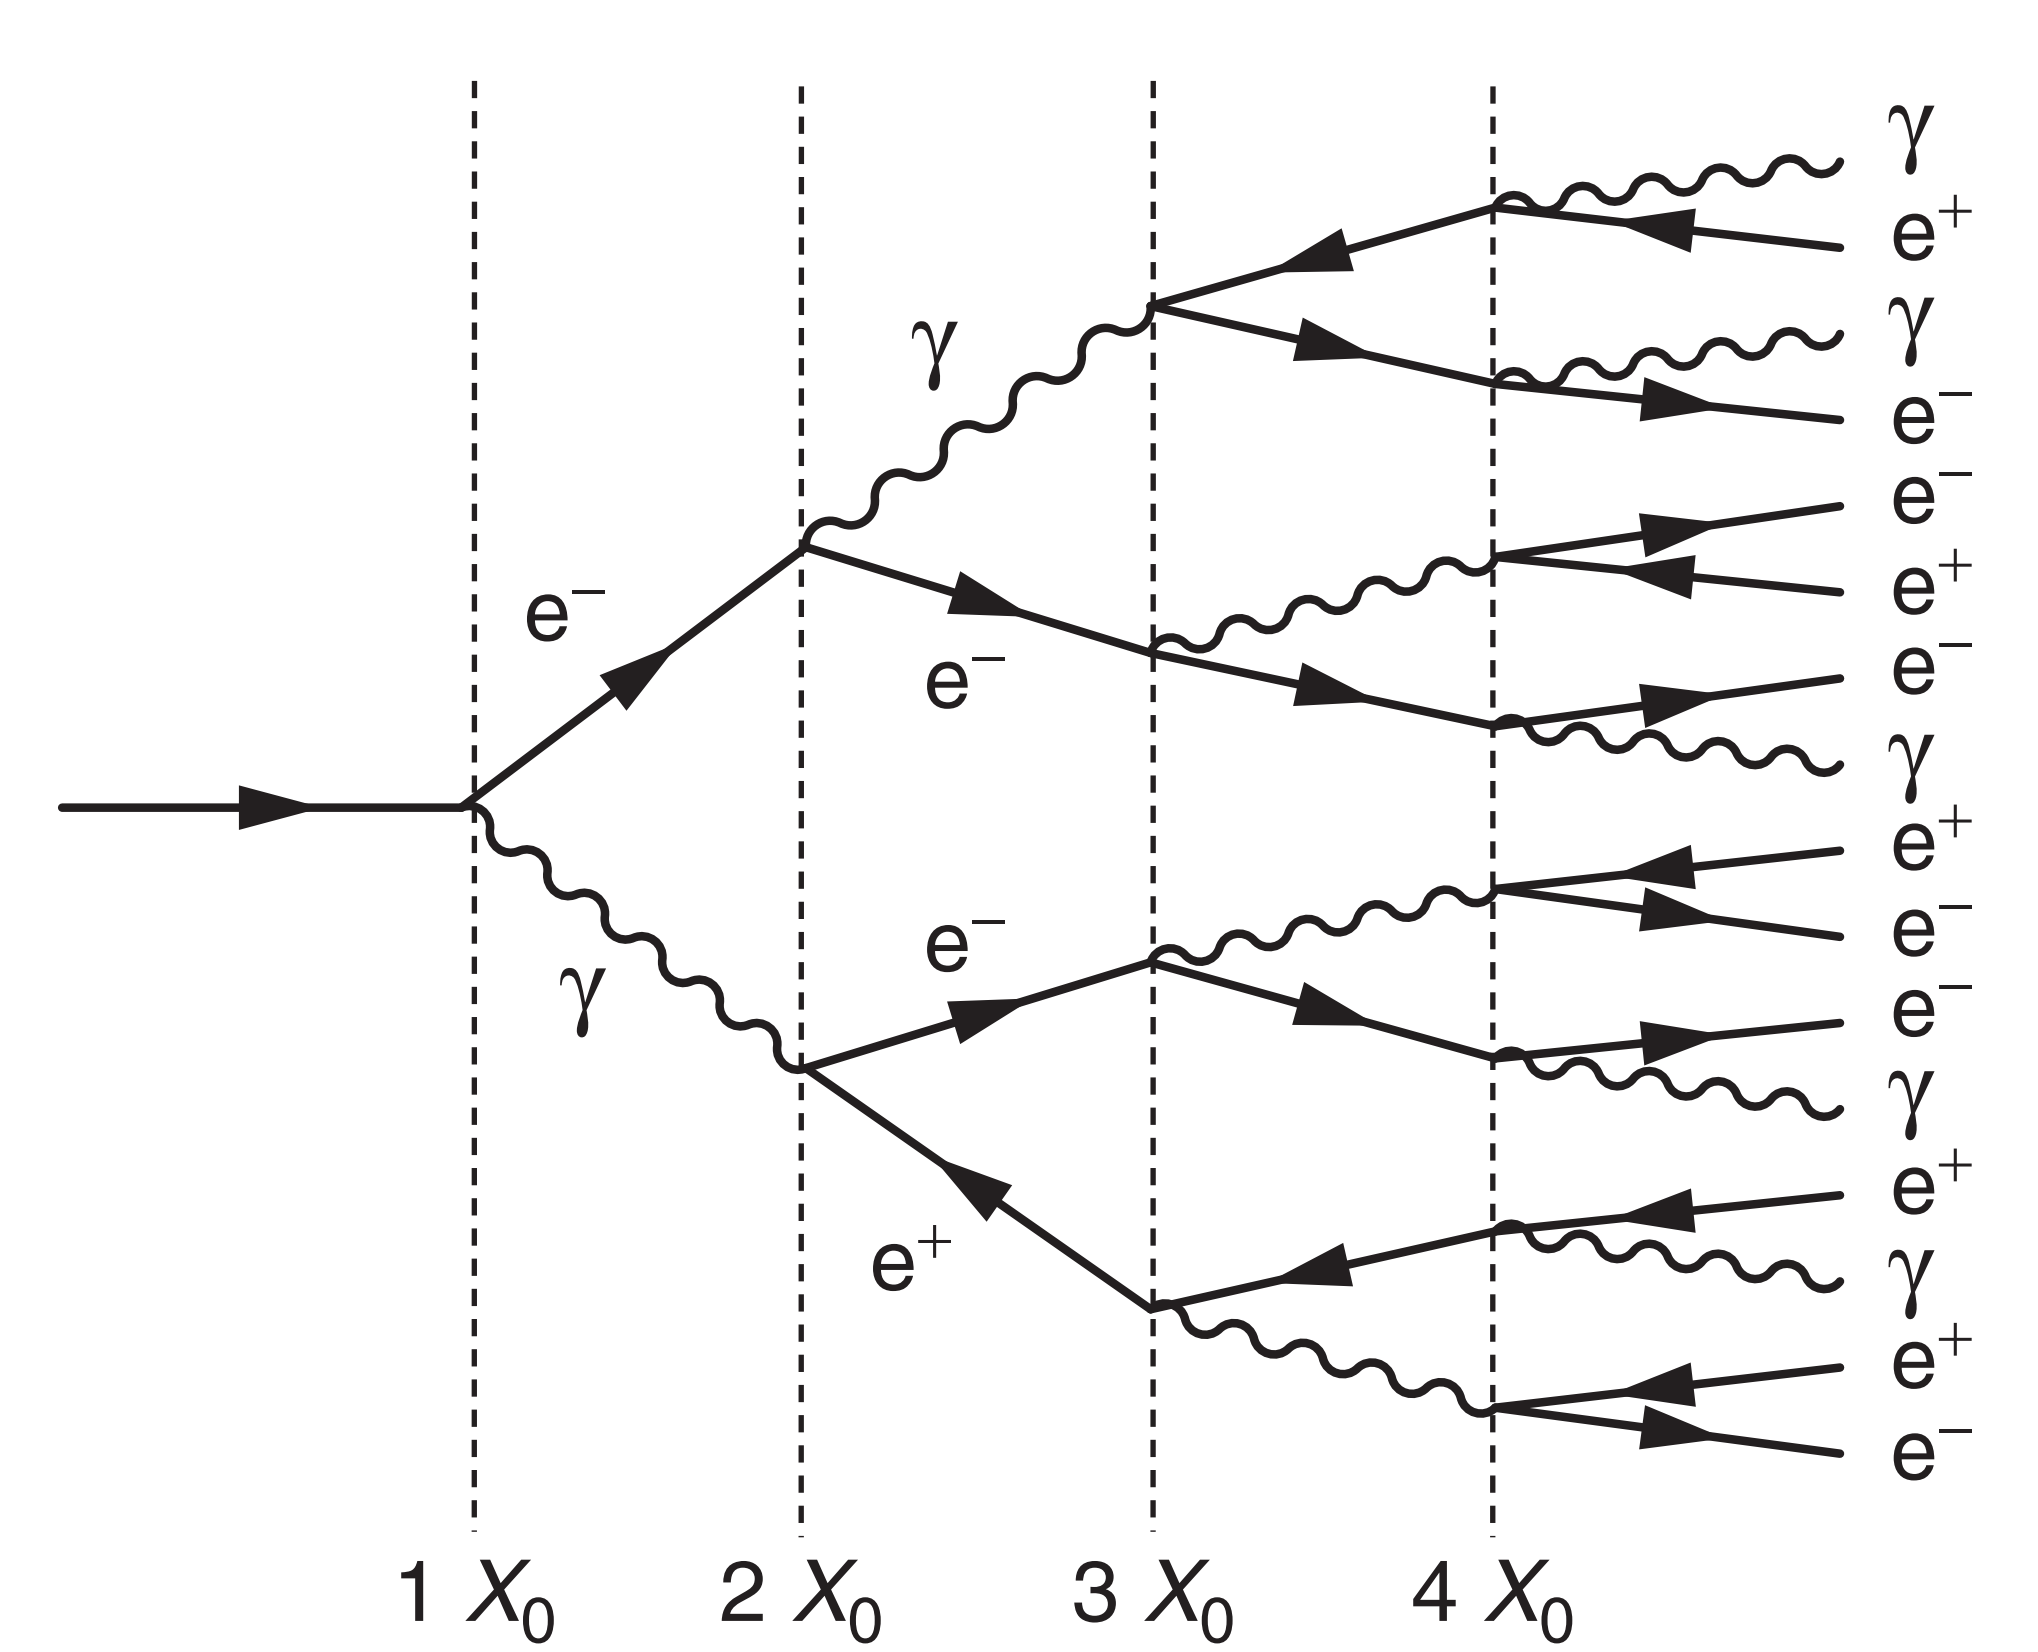
\includegraphics[width=5.2cm, height=4cm]{figs/EMShowers.png}
\end{center}
\end{figure}
\end{column}
	\begin{column}{0.52 \textwidth}
	\justifying
	Although quite fragile and sensitive to the temperature, the short radiation length $X_0$ of the PbWO$_4$ crystals is an advantage, along with their scintillation decay time smaller than the bunch crossing.  \\ \vspace{10pt}
	Each crystal measures 2.2 x 2.2 x 23 cm, corresponding to 26 radiation lengths.
	\end{column}
	\end{columns} \vfill
\end{frame}

\begin{frame}{CMS hadronic calorimeter I}
\justifying
\vspace{10pt}
Charged hadrons lose energy when they traverse matter due to the ionization process resulting from the strong interaction between them and the nuclei of the detector. \vfill
Showers of particles are typically produced since the primary hadronic interaction will produce several additional hadrons, themselves interacting even more with the detector. \vfill

\begin{columns}
	\begin{column}{0.52 \textwidth}
The HCAL is made out of alternating layers:
\vspace{-10pt}
\begin{itemize}
\justifying
\item Of thick \alert{absorber material}, in which the showers can develop;
\item And thin layers of \alert{active material} used for the actual detection by sampling the energy deposition.
\end{itemize}
\end{column}
	\begin{column}{0.45 \textwidth}
	\begin{center}
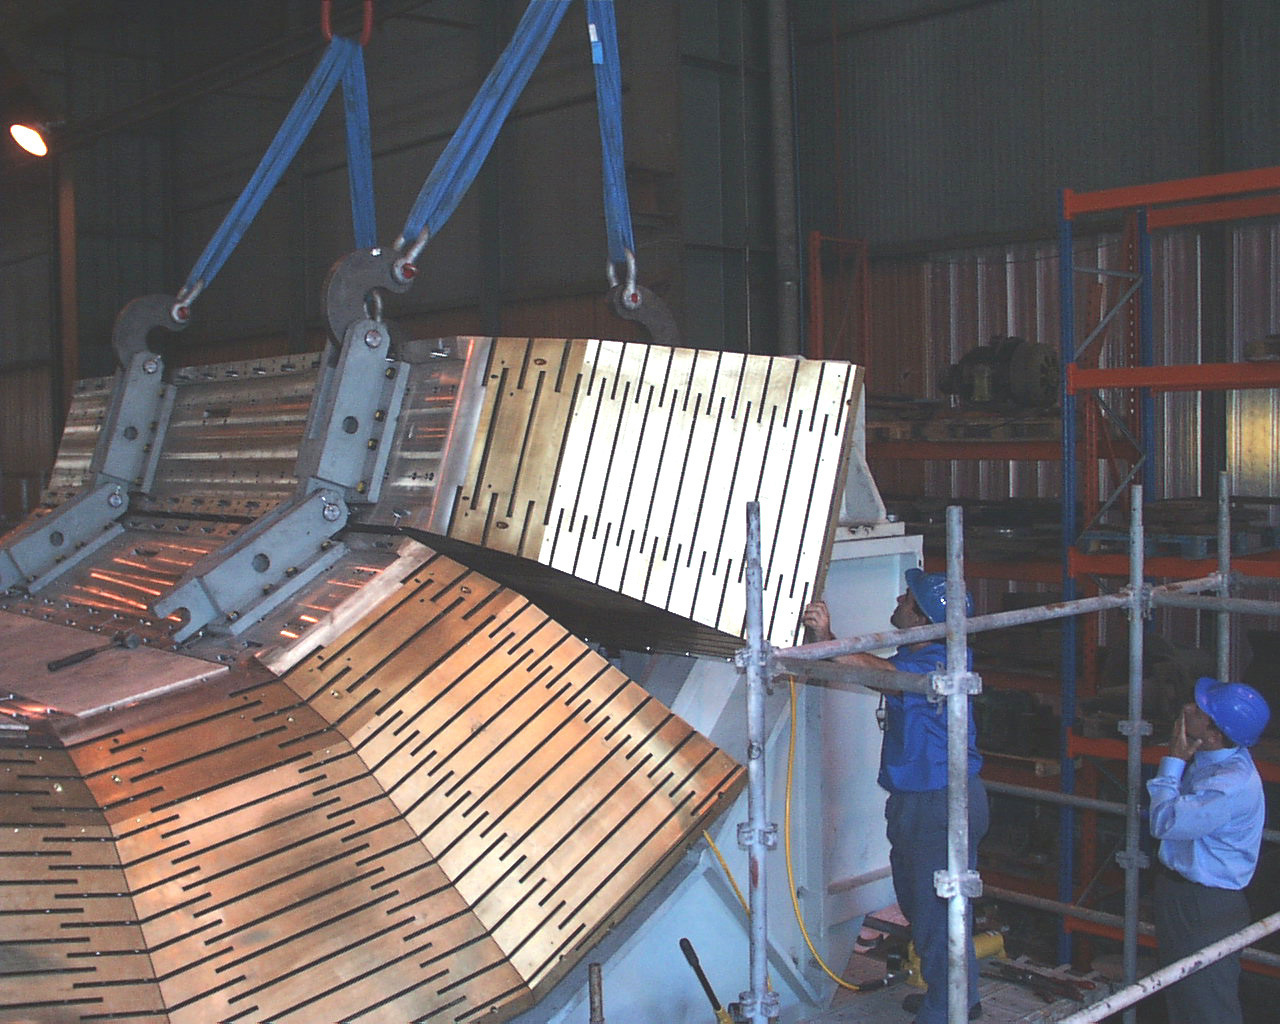
\includegraphics[width=5.2cm, height=4cm]{figs/CMSHcal.jpg}
\end{center}
	\end{column}
	\end{columns} \vfill
\end{frame}

\begin{frame}{CMS hadronic calorimeter II}
\justifying
\vspace{5pt}
The HCAL is divided into:
\begin{itemize}
\item A barrel (HB), up to $|\eta| = 1.3$;
\item Two endcaps, extending the pseudorapidities coverage up to $|\eta| = 3.0$;
\item Two symmetrical forward regions (HF), covering up to $|\eta| = 5.2$;
\item And the Hadron Outer (HO), outside of the solenoid, placed to increase the effective nuclear radiation length $\lambda$, otherwise low at a $90^{\circ}$ incidence angle.
\end{itemize} \vfill

\begin{figure}[htbp]
\begin{center}
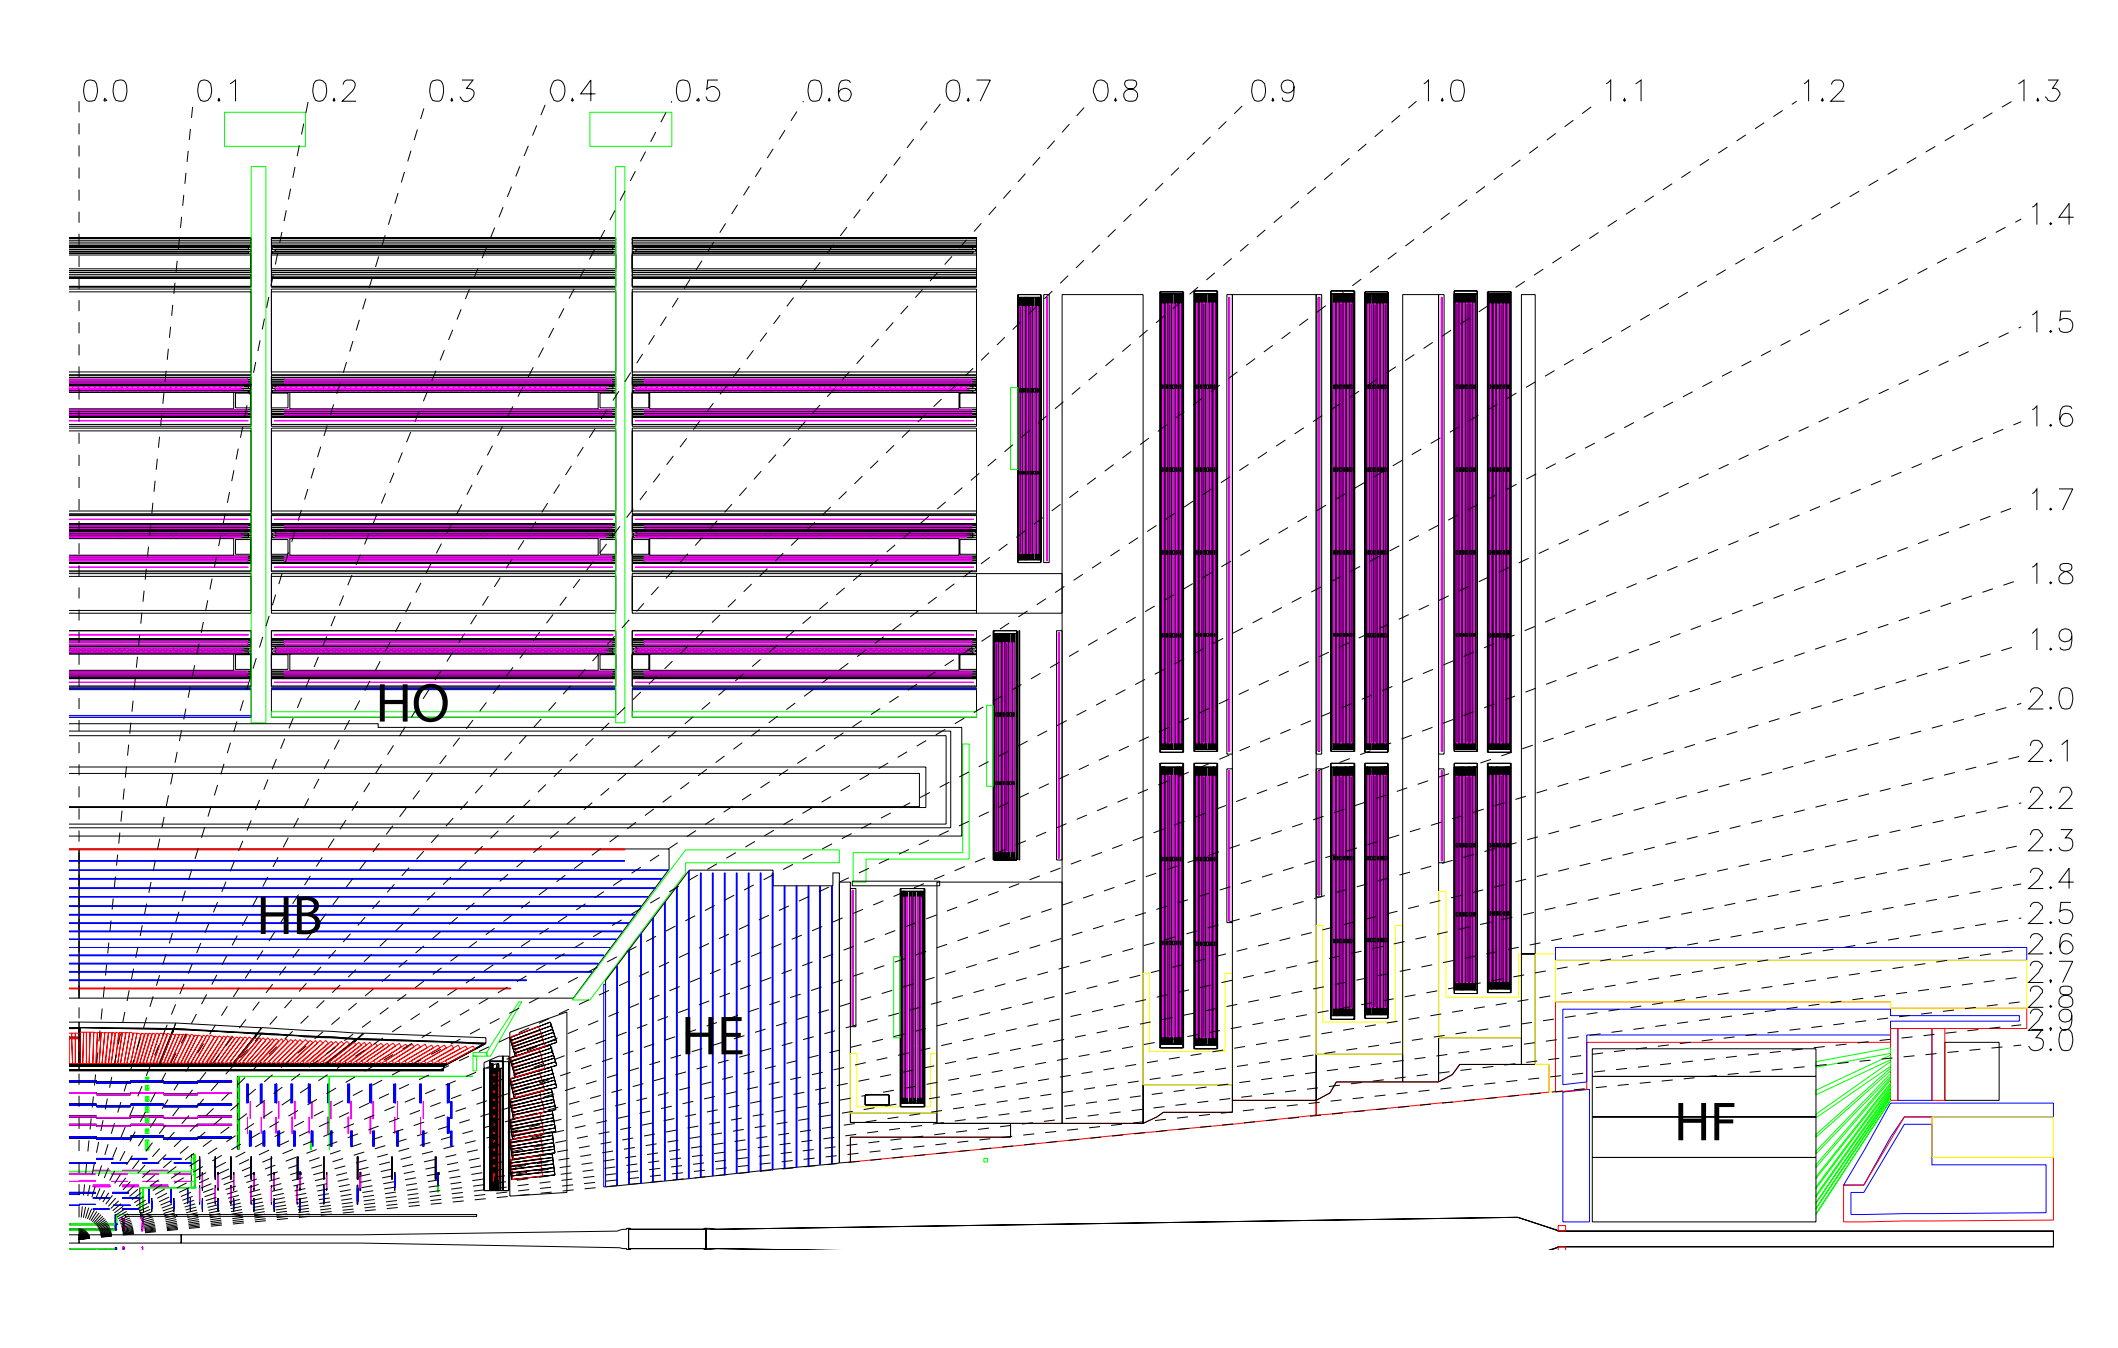
\includegraphics[width=8.2cm, height=5.2cm]{figs/CMSHCAL.png}
\end{center}
\end{figure}
\end{frame}

\begin{frame}{CMS solenoid}
\justifying
\begin{columns}
	\begin{column}{0.46 \textwidth}
	\justifying
The superconducting solenoid:
\begin{itemize}
\justifying
\item Is made out of 6 endcap disks and 5 barrel wheels;
\item Weights more than 12 000 tons in total, with the return yoke;
\item Is able to produce a 3.8T magnetic field once cooled down to 4.5K;
\item Stores at all times around 2.6GJ of energy.
\end{itemize}
\end{column}
	\begin{column}{0.51 \textwidth}
\begin{figure}[htbp]
\begin{center}
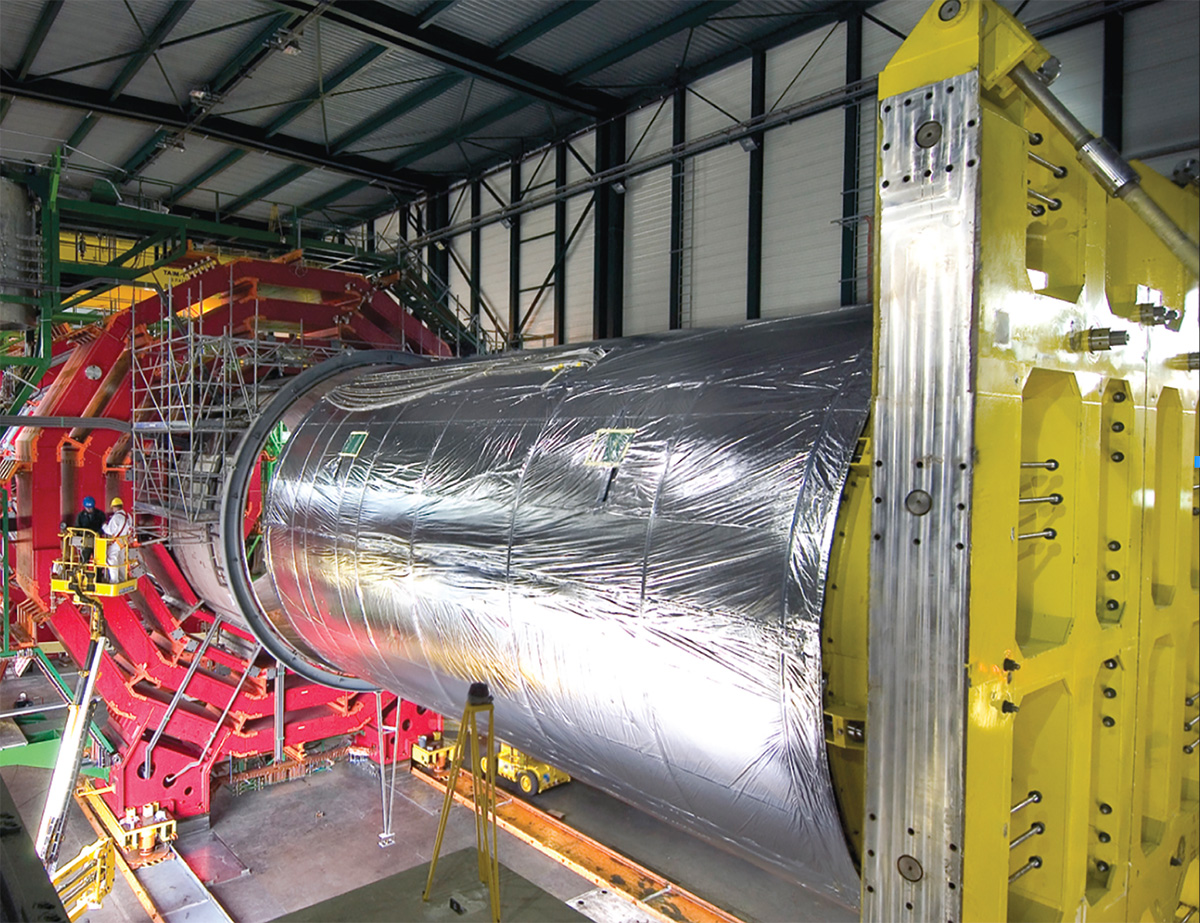
\includegraphics[width=5.5cm, height=3.7cm]{figs/CMSMagnet.jpg}
\end{center}
\end{figure}
	\end{column}
	\end{columns} \vfill

It allows the measurement of the momentum and charge of particles by studying the curvature of their tracks, according to the Lorentz equation:

\begin{equation*}
\overrightarrow{F} = \frac{m \overrightarrow{v}^2}{R} =  q \overrightarrow{E} + q \overrightarrow{v} \times \overrightarrow{B} = q \overrightarrow{v} \times \overrightarrow{B}
\end{equation*}
\vfill

It has been designed to reach a momentum resolution $\Delta p/p \sim 10$\% at $p = 1$ TeV. \vfill
\end{frame}

\begin{frame}{CMS muon systems I}
\justifying
The muon systems is the outtermost section of CMS, covering around 25 000 m$^2$. \vfill 

Three different categories of devices have been designed, in order to cope with the specific experimental conditions in the different parts of the detector: the Drift Tubes (DTs), the Cathode Strips Chambers (CSCs), and the Resistive Plate Chambers (RPCs). \vfill

\begin{center}
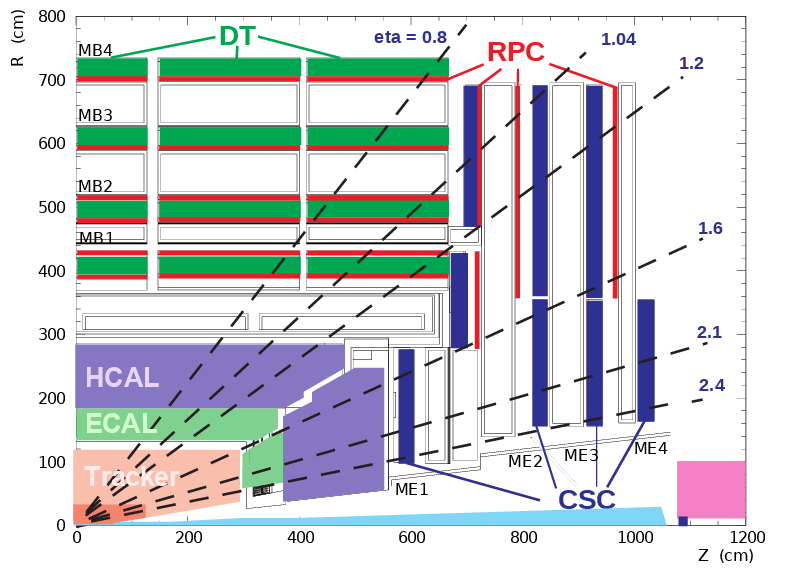
\includegraphics[width=8cm, height=4.9cm]{figs/CMSMuons.png}
\end{center} \vfill

All these detectors are gaseous, distributed over a cylindrical area given the shape of the innermost components of CMS, and cheap, given the large surface they cover. \vfill
\end{frame}

\begin{frame}{CMS muon systems II}
Comparison of the different subsystems:
\begin{table}[h!]
\begin{center}
\resizebox{\textwidth}{!}{
\begin{tabular}{ c|c|c|c } 
 \hline
 Muon sub-system & DTs & CSCs & RPCs \\
 \hline
 $|\eta|$ coverage & 0.0-1.2 & 0.9-2.4 & 0.0-1.9 \\
 Stations & 4 & 4 & 4 \\
 Chambers & 250 & 540 & \makecell{\vspace{-10pt} \\ 480 (barrel) \\ 576 (endcaps)} \\
 Readout channels & 172 000 & \makecell{\vspace{-10pt} \\ 266 112 (strips) \\ 210 816 (anode channels)} & \makecell{\vspace{-10pt} \\ 68 136 (barrel) \\ 55 296 (endcaps)} \\
 Spatial resolution & 80-120 $\mu$m & 40-150 $\mu$m & 0.8-1.2 cm \\
 Average efficiency (13 TeV) & 97.1\% & $97.4$\% & \makecell{\vspace{-10pt} \\ 94.2\% (barrel) \\ 96.4\% (endcaps)} \\ 
 \hline
\end{tabular}
}
\end{center}
\end{table}
\end{frame}

\begin{frame}{CMS DTs}
\justifying
\vspace{5pt}
Placed in the barrel region (up to $|\eta| = 1.2$), where the background levels and magnetic field are low, this system allows a good efficiency for the muon hits reconstruction into a single track and a good rejection of eventual background hits. \vfill

\begin{columns}
	\begin{column}{0.48 \textwidth}
	\justifying
This system is:
\begin{itemize}
\justifying
\item Able to collect the residuals charges left by the ionization tracks of muons;
\item Made out of 172 000 sensitive wires, divided in 250 chambers;
\item Redundant, by the installation of 4 layers, to reduce the impact coming from eventual neutrons or photons;
\item Has a maximal drift time of 380ns, low enough to avoid the need of multi-hits electronics.
\end{itemize}
\end{column}
	\begin{column}{0.51 \textwidth}
\begin{figure}[htbp]
\begin{center}
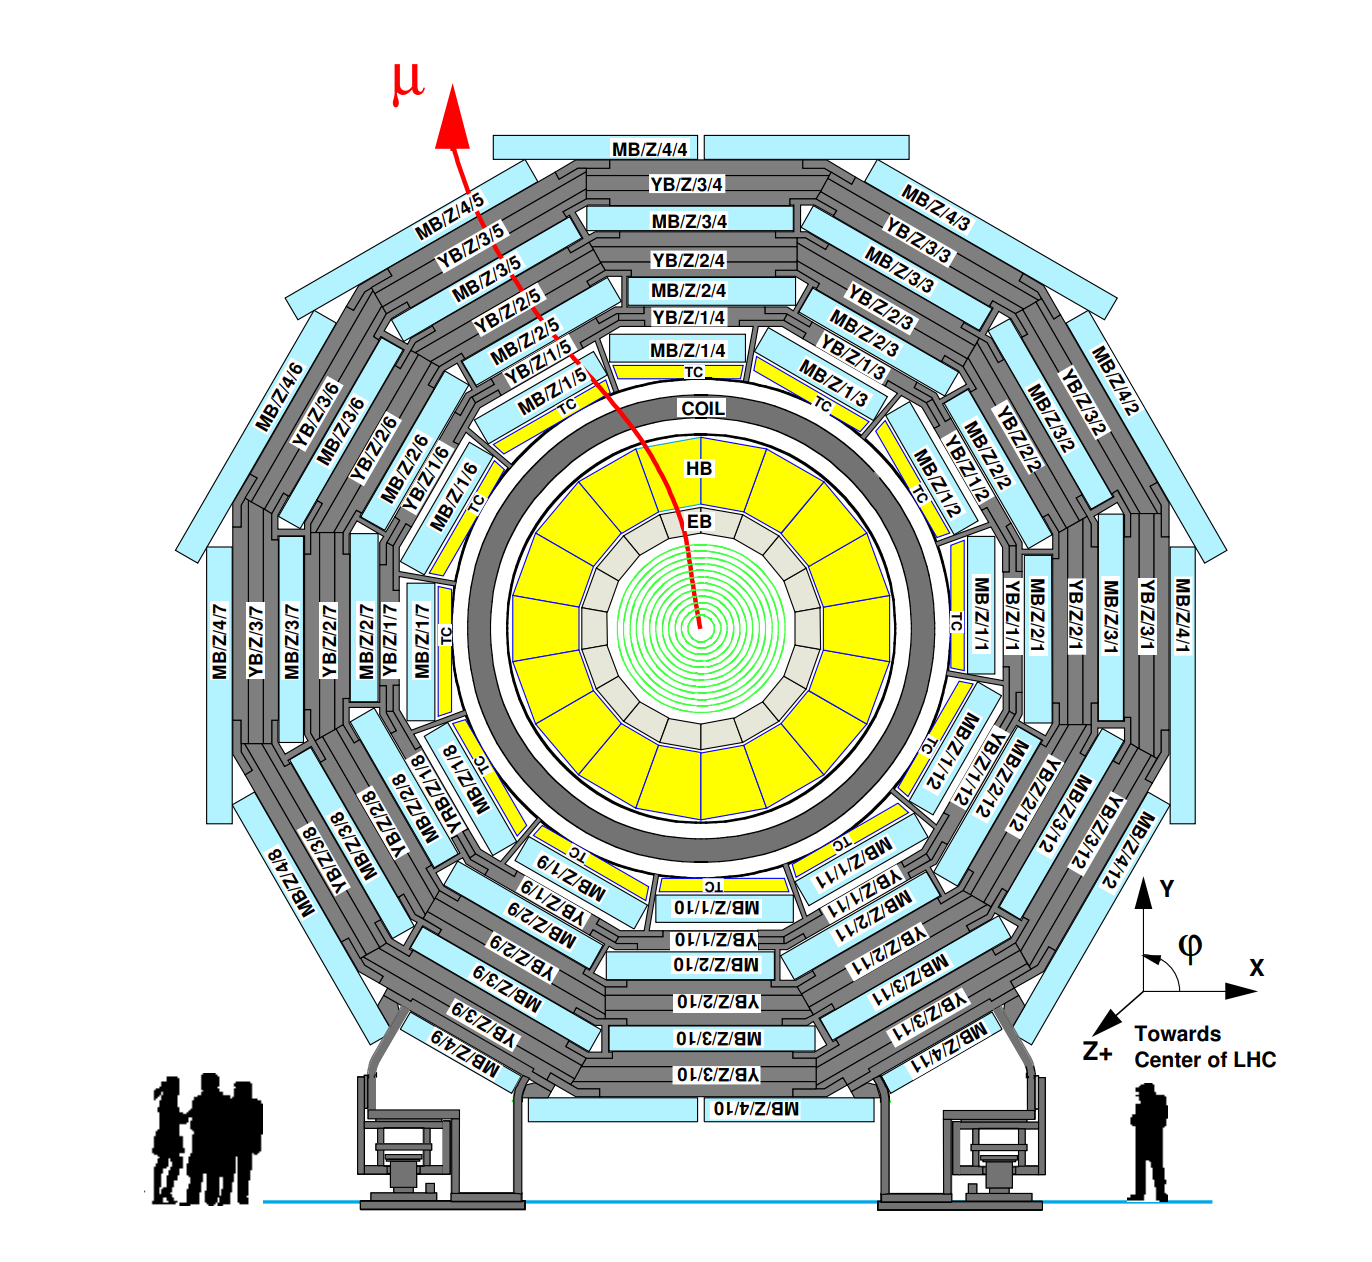
\includegraphics[width=6cm, height=5.2cm]{figs/CMSDT.png}
\end{center}
\end{figure}
	\end{column}
	\end{columns} \vfill
\end{frame}

\begin{frame}{2016 data samples}
\justifying
\begin{table}
\begin{center}
\resizebox{0.65\textwidth}{!}{
\begin{tabular}{ c|c|c } 
 \hline
 Dataset & Events (size) & $\mathcal{L}$ [fb$^{-1}$] \\
\hline
\textbf{Run 2016B} & & \\
/DoubleEG/Run2016B\_ver2-Nano02Apr2020\_ver2-v1/NANOAOD & 143073268 (99.4Gb) & \multirow{ 5}{*}{5.8}  \\
/DoubleMuon/Run2016B\_ver2-Nano02Apr2020\_ver2-v1/NANOAOD & 82535526 (53.2Gb) &   \\
 /MuonEG/Run2016B\_ver2-Nano02Apr2020\_ver2-v1/NANOAOD & 32727796 (26.8Gb) & \\
 /SingleElectron/Run2016B\_ver2-Nano02Apr2020\_ver2-v1/NANOAOD & 246440440 (167.8Gb) & \\
 /SingleMuon/Run2016B\_ver2-Nano02Apr2020\_ver2-v1/NANOAOD & 158145722 (96.4Gb) & \\
 \hline
 \textbf{Run 2016C} & & \\
 /DoubleEG/Run2016C-Nano02Apr2020-v1/NANOAOD & 47677856 (35.3Gb) & \multirow{ 5}{*}{2.6} \\
 /DoubleMuon/Run2016C-Nano02Apr2020-v1/NANOAOD & 27934629 (19.7Gb) & \\
 /MuonEG/Run2016C-Nano02Apr2020-v1/NANOAOD & 15405678 (12.8Gb) & \\
 /SingleElectron/Run2016C-Nano02Apr2020-v1/NANOAOD & 97259854 (69.3Gb) & \\
 /SingleMuon/Run2016C-Nano02Apr2020-v1/NANOAOD & 67441308 (42.4Gb) & \\
 \hline
 \textbf{Run 2016D} & & \\
 /DoubleEG/Run2016D-Nano02Apr2020-v1/NANOAOD & 53324960 (39.6Gb) & \multirow{ 5}{*}{4.2} \\
 /DoubleMuon/Run2016D-Nano02Apr2020-v1/NANOAOD & 33861745 (24.1Gb) & \\
 /MuonEG/Run2016D-Nano02Apr2020-v1/NANOAOD & 23482352 (19.4Gb) & \\
 /SingleElectron/Run2016D-Nano02Apr2020-v1/NANOAOD & 148167727 (104.4Gb) & \\
 /SingleMuon/Run2016D-Nano02Apr2020-v1/NANOAOD & 98017996 (61.3Gb) & \\
 \hline
 \textbf{Run 2016E} & & \\
 /DoubleEG/Run2016E-Nano02Apr2020-v1/NANOAOD & 49877710 (37.9Gb) & \multirow{ 5}{*}{4.0} \\
 /DoubleMuon/Run2016E-Nano02Apr2020-v1/NANOAOD & 28246946 (20.8Gb) & \\
 /MuonEG/Run2016E-Nano02Apr2020-v2/NANOAOD & 22519303 (19.0Gb) & \\
 /SingleElectron/Run2016E-Nano02Apr2020-v1/NANOAOD & 117321545 (86.5Gb) & \\
 /SingleMuon/Run2016E-Nano02Apr2020-v1/NANOAOD & 90984718 (58.7Gb) & \\
 \hline
 \textbf{Run 2016F} & & \\
 /DoubleEG/Run2016F-Nano02Apr2020-v1/NANOAOD & 34577629 (26.9Gb) & \multirow{ 5}{*}{3.1} \\
 /DoubleMuon/Run2016F-Nano02Apr2020-v1/NANOAOD & 20329921 (15.3Gb) & \\
 /MuonEG/Run2016F-Nano02Apr2020-v1/NANOAOD & 16002165 (13.6Gb) & \\
 /SingleElectron/Run2016F-Nano02Apr2020-v1/NANOAOD & 70593532 (51.4Gb) & \\
 /SingleMuon/Run2016F-Nano02Apr2020-v1/NANOAOD & 65489554 (42.4Gb) & \\
 \hline
 \textbf{Run 2016G} & & \\
 /DoubleEG/Run2016G-Nano02Apr2020-v1/NANOAOD & 78797031 (61.6Gb) & \multirow{ 5}{*}{7.6} \\
 /DoubleMuon/Run2016G-Nano02Apr2020-v1/NANOAOD & 45235604 (34.2Gb) & \\
 /MuonEG/Run2016G-Nano02Apr2020-v1/NANOAOD & 33854612 (29.0Gb) & \\
 /SingleElectron/Run2016G-Nano02Apr2020-v1/NANOAOD & 153363109 (109.2Gb) & \\
 /SingleMuon/Run2016G-Nano02Apr2020-v1/NANOAOD & 149912248 (94.6Gb) & \\
 \hline
 \textbf{Run 2016H} & & \\
 /DoubleEG/Run2016H-Nano02Apr2020-v1/NANOAOD & 85388734 (67.7Gb) & \multirow{ 5}{*}{8.6} \\
 /DoubleMuon/Run2016H-Nano02Apr2020-v1/NANOAOD & 48912812 (37.3Gb) & \\
 /MuonEG/Run2016H-Nano02Apr2020-v1/NANOAOD & 29236516 (26.0Gb) & \\
 /SingleElectron/Run2016H-Nano02Apr2020-v1/NANOAOD & 128854598 (93.8Gb) & \\
 /SingleMuon/Run2016H-Nano02Apr2020-v1/NANOAOD & 174035164 (110.2Gb) & \\
 \hline
\end{tabular}
}
\end{center}
\end{table}
\end{frame}

\begin{frame}{2017 data samples}
\justifying
\begin{table}
\begin{center}
\resizebox{0.8\textwidth}{!}{
\begin{tabular}{ c|c|c } 
 \hline
 Dataset & Events (size) & $\mathcal{L}$ [fb$^{-1}$] \\
\hline
\textbf{Run 2017B} & & \\
/DoubleEG/Run2017B-Nano02Apr2020-v1/NANOAOD & 58088760 (46.6Gb) & \multirow{ 5}{*}{4.8} \\
/DoubleMuon/Run2017B-Nano02Apr2020-v1/NANOAOD & 14501767 (10.8Gb) & \\
/SingleElectron/Run2017B-Nano02Apr2020-v1/NANOAOD & 60537490 (42.2Gb) & \\
/SingleMuon/Run2017B-Nano02Apr2020-v1/NANOAOD & 136300266 (86.2Gb) & \\
/MuonEG/Run2017B-Nano02Apr2020-v1/NANOAOD & 4453465 (4.1Gb) & \\
 \hline
 \textbf{Run 2017C} & & \\
 /DoubleEG/Run2017C-Nano02Apr2020-v1/NANOAOD & 65181125 (53.8Gb) & \multirow{ 5}{*}{9.7} \\
 /DoubleMuon/Run2017C-Nano02Apr2020-v1/NANOAOD & 49636525 (39.5Gb) & \\
 /SingleElectron/Run2017C-Nano02Apr2020-v1/NANOAOD & 136637888 (102.5Gb) & \\
 /SingleMuon/Run2017C-Nano02Apr2020-v1/NANOAOD & 165652756 (109.5Gb) & \\
 /MuonEG/Run2017C-Nano02Apr2020-v1/NANOAOD & 15595214 (15.0Gb) & \\
 \hline
 \textbf{Run 2017D} & & \\
/DoubleEG/Run2017D-Nano02Apr2020-v1/NANOAOD & 25911432 (21.6Gb) & \multirow{ 5}{*}{4.2} \\
/DoubleMuon/Run2017D-Nano02Apr2020-v1/NANOAOD & 23075733 (18.6Gb) & \\
/SingleElectron/Run2017D-Nano02Apr2020-v1/NANOAOD & 51526710 (38.5Gb) & \\
/SingleMuon/Run2017D-Nano02Apr2020-v1/NANOAOD & 70361660 (47.2Gb) & \\
 /MuonEG/Run2017D-Nano02Apr2020-v1/NANOAOD & 9164365 (8.9Gb) & \\
 \hline
 \textbf{Run 2017E} & & \\
/DoubleEG/Run2017E-Nano02Apr2020-v1/NANOAOD & 56233597 (49.8Gb) & \multirow{ 5}{*}{9.3} \\
/DoubleMuon/Run2017E-Nano02Apr2020-v1/NANOAOD & 51589091 (44.4Gb) & \\
/SingleElectron/Run2017E-Nano02Apr2020-v1/NANOAOD & 102121689 (81.3Gb) & \\
/SingleMuon/Run2017E-Nano02Apr2020-v1/NANOAOD & 154630534 (111.0Gb) & \\
/MuonEG/Run2017E-Nano02Apr2020-v1/NANOAOD & 19043421 (19.2Gb) & \\
 \hline
\textbf{Run 2017F} & & \\ 
/DoubleEG/Run2017F-Nano02Apr2020-v1/NANOAOD & 74307066 (67.1Gb) & \multirow{ 5}{*}{13.5} \\
/DoubleMuon/Run2017F-Nano02Apr2020-v1/NANOAOD & 79756560 (68.0Gb) & \\
/SingleElectron/Run2017F-Nano02Apr2020-v1/NANOAOD & 128467223 (105.2Gb) & \\
/SingleMuon/Run2017F-Nano02Apr2020-v1/NANOAOD & 242135500 (178.3Gb) \\
 /MuonEG/Run2017F-Nano02Apr2020-v1/NANOAOD & 25776363 (26.3Gb) & \\
 \hline
\end{tabular}
}
\end{center}
\end{table}
\end{frame}

\begin{frame}{2018 data samples}
\justifying
\begin{table}
\begin{center}
\resizebox{0.8\textwidth}{!}{
\begin{tabular}{ c|c|c } 
 \hline
 Dataset & Events (size) & $\mathcal{L}$ [fb$^{-1}$] \\
\hline
\textbf{Run 2018A} & & \\
 /DoubleMuon/Run2018A-Nano02Apr2020-v1/NANOAOD & 75499908 (62.6Gb) & \multirow{ 4}{*}{13.5} \\
 /EGamma/Run2018A-Nano02Apr2020-v1/NANOAOD & 327843843 (261.8Gb) & \\
 /SingleMuon/Run2018A-Nano02Apr2020-v1/NANOAOD & 241608232 (167.7Gb) & \\
 /MuonEG/Run2018A-Nano02Apr2020-v1/NANOAOD & 32958503 (32.3Gb) & \\
 \hline
\textbf{Run 2018B} & & \\
 /DoubleMuon/Run2018B-Nano02Apr2020-v1/NANOAOD & 35057758 (28.3Gb) & \multirow{ 4}{*}{6.8} \\
 /EGamma/Run2018B-Nano02Apr2020-v1/NANOAOD & 153822427 (123.1Gb) & \\
 /SingleMuon/Run2018B-Nano02Apr2020-v1/NANOAOD & 119918017 (82.3Gb) & \\
 /MuonEG/Run2018B-Nano02Apr2020-v1/NANOAOD & 16211567 (15.8Gb) & \\
 \hline
 \textbf{Run 2018C} & & \\
/DoubleMuon/Run2018C-Nano02Apr2020-v1/NANOAOD & 34565869 (27.6Gb) & \multirow{ 4}{*}{6.6} \\
/EGamma/Run2018C-Nano02Apr2020-v1/NANOAOD & 147827904 (119.2Gb) & \\
/SingleMuon/Run2018C-Nano02Apr2020-v1/NANOAOD & 110032072 (75.7Gb) & \\
/MuonEG/Run2018C-Nano02Apr2020-v1/NANOAOD & 15652198 (15.3Gb) & \\
 \hline
 \textbf{Run 2018D} & & \\
/DoubleMuon/Run2018D-Nano02Apr2020\_ver2-v1/NANOAOD & 168605834 (128.6Gb) & \multirow{ 4}{*}{32.0} \\
/EGamma/Run2018D-Nano02Apr2020-v1/NANOAOD & 751348648 (583.6Gb) & \\
/SingleMuon/Run2018D-Nano02Apr2020-v1/NANOAOD & 513867253 (344.5Gb) & \\
/MuonEG/Run2018D-Nano02Apr2020\_ver2-v1/NANOAOD & 71961587 (68.6Gb) & \\
 \hline
\end{tabular}
}
\end{center}
\end{table}
\end{frame}

\begin{frame}{2016 MC samples}
\justifying
\begin{table}
\begin{center}
\resizebox{0.9\textwidth}{!}{
\begin{tabular}{ c|c|c } 
 \hline
 Process & Sample & Cross section [pb] \\
\hline
\multirow{1}{*}{Drell-Yan} & DYJetsToLL\_M-10to50\_TuneCUETP8M1\_13TeV-madgraphMLM-pythia8 ($H_T < 70$ GeV) & 18610.0 \\
& DYJetsToLL\_M-5to50\_HT-70to100\_TuneCUETP8M1\_13TeV-madgraphMLM-pythia8 & 303.8 \\
& DYJetsToLL\_M-5to50\_HT-100to200\_TuneCUETP8M1\_13TeV-madgraphMLM-pythia8 & 224.2 \\
& DYJetsToLL\_M-5to50\_HT-200to400\_TuneCUETP8M1\_13TeV-madgraphMLM-pythia8 & 37.2 \\
& DYJetsToLL\_M-5to50\_HT-400to600\_TuneCUETP8M1\_13TeV-madgraphMLM-pythia8 & 3.581 \\
& DYJetsToLL\_M-5to50\_HT-600toInf\_TuneCUETP8M1\_13TeV-madgraphMLM-pythia8 & 1.124 \\
& DYJetsToLL\_M-50\_TuneCUETP8M1\_13TeV-madgraphMLM-pythia8 ($H_T < 70$ GeV) & 6025.20 \\
& DYJetsToLL\_M-50\_HT-70to100\_TuneCUETP8M1\_13TeV-madgraphMLM-pythia8 & 169.9 \\
& DYJetsToLL\_M-50\_HT-100to200\_TuneCUETP8M1\_13TeV-madgraphMLM-pythia8 & 147.4 \\
& DYJetsToLL\_M-50\_HT-200to400\_TuneCUETP8M1\_13TeV-madgraphMLM-pythia8 & 40.99 \\
& DYJetsToLL\_M-50\_HT-400to600\_TuneCUETP8M1\_13TeV-madgraphMLM-pythia8 & 5.678 \\
& DYJetsToLL\_M-50\_HT-600to800\_TuneCUETP8M1\_13TeV-madgraphMLM-pythia8 & 1.367 \\
& DYJetsToLL\_M-50\_HT-800to1200\_TuneCUETP8M1\_13TeV-madgraphMLM-pythia8 & 0.6304 \\
& DYJetsToLL\_M-50\_HT-1200to2500\_TuneCUETP8M1\_13TeV-madgraphMLM-pythia8 & 0.1514 \\
& DYJetsToLL\_M-50\_HT-2500toInf\_TuneCUETP8M1\_13TeV-madgraphMLM-pythia8 & 0.003565 \\
\hline
\multirow{1}{*}{TTTo2L2Nu} & TTTo2L2Nu\_TuneCUETP8M2\_ttHtranche3\_13TeV-powheg-pythia8 & 87.310 \\
\hline
\multirow{1}{*}{Single top} & ST\_s-channel\_4f\_leptonDecays\_13TeV-amcatnlo-pythia8\_TuneCUETP8M1 & 3.360 \\
& ST\_t-channel\_antitop\_4f\_inclusiveDecays\_13TeV-powhegV2-madspin-pythia8\_TuneCUETP8M1 & 80.95 \\
& ST\_t-channel\_top\_4f\_inclusiveDecays\_13TeV-powhegV2-madspin-pythia8\_TuneCUETP8M1 & 136.02 \\
& ST\_tW\_antitop\_5f\_inclusiveDecays\_13TeV-powheg-pythia8\_TuneCUETP8M1 & 35.60 \\
& ST\_tW\_top\_5f\_inclusiveDecays\_13TeV-powheg-pythia8\_TuneCUETP8M1 & 35.60 \\
\hline
WW & WWTo2L2Nu\_13TeV-powheg & 12.178 \\
& WWJJToLNuLNu\_EWK\_noTop\_13TeV-madgraph-pythia8 & 0.34520 \\
& GluGluWWTo2L2Nu\_MCFM\_13TeV & 0.5905 \\
\hline
V$\gamma$/V$\gamma$* & WGToLNuG\_TuneCUETP8M1\_13TeV-madgraphMLM-pythia8 & 405.271 \\ 
& ZGTo2LG\_TuneCUETP8M1\_13TeV-amcatnloFXFX-pythia8 & 131.300 \\
& WZTo3LNu\_mllmin01\_13TeV-powheg-pythia8 & 58.59 \\
\hline
VZ & ZZTo2L2Nu\_13TeV\_powheg\_pythia8 & 0.5640 \\
& ZZTo2L2Q\_13TeV\_powheg\_pythia8 & 3.22 \\
& ZZTo4L\_TuneCP5\_13TeV\_powheg\_pythia8 & 1.212 \\
& WZTo2L2Q\_13TeV\_amcatnloFXFX\_madspin\_pythia8 & 5.595 \\
 \hline
 VVV & ZZZ\_TuneCUETP8M1\_13TeV-amcatnlo-pythia8 & 0.01398 \\
 & WZZ\_TuneCUETP8M1\_13TeV-amcatnlo-pythia8 & 0.05565 \\
 & WWZ\_TuneCUETP8M1\_13TeV-amcatnlo-pythia8 & 0.16510 \\
 & WWW\_4F\_TuneCUETP8M1\_13TeV-amcatnlo-pythia8 & 0.18331 \\
 \hline
 Non-Prompt & Data-driven (tight-to-loose method) & \\
 \hline
\end{tabular}
}
\end{center}
\end{table}
\end{frame}

\begin{frame}{2017 MC samples}
\justifying
\begin{table}
\begin{center}
\resizebox{0.9\textwidth}{!}{
\begin{tabular}{ c|c|c } 
 \hline
 Process & Sample & Cross section [pb] \\
\hline
\multirow{1}{*}{Drell-Yan} & DYJetsToLL\_M-10to50\_TuneCP5\_13TeV-madgraphMLM-pythia8 ($H_T < 100$ GeV) & 18610 \\
& DYJetsToLL\_M-4to50\_HT-100to200\_TuneCP5\_13TeV-madgraphMLM-pythia8 & 204.0 \\
& DYJetsToLL\_M-4to50\_HT-200to400\_TuneCP5\_13TeV-madgraphMLM-pythia8 & 54.39 \\
& DYJetsToLL\_M-4to50\_HT-400to600\_TuneCP5\_13TeV-madgraphMLM-pythia8 & 5.697 \\
& DYJetsToLL\_M-4to50\_HT-600toInf\_TuneCP5\_13TeV-madgraphMLM-pythia8 & 1.85 \\
& DYJetsToLL\_M-50\_TuneCP5\_13TeV-madgraphMLM-pythia8 ($H_T < 70$ GeV) & 6189.39 \\
& DYJetsToLL\_M-50\_HT-70to100\_TuneCP5\_13TeV-madgraphMLM-pythia8 & 169.9 \\
& DYJetsToLL\_M-50\_HT-100to200\_TuneCP5\_13TeV-madgraphMLM-pythia8 & 161.1 \\
& DYJetsToLL\_M-50\_HT-200to400\_TuneCP5\_13TeV-madgraphMLM-pythia8 & 48.66 \\
& DYJetsToLL\_M-50\_HT-400to600\_TuneCP5\_13TeV-madgraphMLM-pythia8 & 6.968 \\
& DYJetsToLL\_M-50\_HT-600to800\_TuneCP5\_13TeV-madgraphMLM-pythia8 & 1.743 \\
& DYJetsToLL\_M-50\_HT-800to1200\_TuneCP5\_13TeV-madgraphMLM-pythia8 & 0.8052 \\
& DYJetsToLL\_M-50\_HT-1200to2500\_TuneCP5\_13TeV-madgraphMLM-pythia8 & 0.1933 \\
& DYJetsToLL\_M-50\_HT-2500toInf\_TuneCP5\_13TeV-madgraphMLM-pythia8 & 0.003468 \\
\hline
\multirow{1}{*}{TTTo2L2Nu} & TTTo2L2Nu\_TuneCP5\_13TeV-powheg-pythia8 & 87.310 \\
\hline
\multirow{1}{*}{Single top} & ST\_s-channel\_4f\_leptonDecays\_mtop1715\_TuneCP5\_PSweights\_13TeV-amcatnlo-pythia8 & 3.360 \\
& ST\_t-channel\_antitop\_4f\_inclusiveDecays\_TuneCP5\_13TeV-powhegV2-madspin-pythia8 & 80.95 \\
& ST\_t-channel\_top\_4f\_inclusiveDecays\_TuneCP5\_13TeV-powhegV2-madspin-pythia8 & 136.02 \\
& ST\_tW\_antitop\_5f\_inclusiveDecays\_TuneCP5\_13TeV-powheg-pythia8 & 35.60 \\
& ST\_tW\_top\_5f\_inclusiveDecays\_TuneCP5\_13TeV-powheg-pythia8 & 35.60 \\
\hline
WW & WWTo2L2Nu\_NNPDF31\_TuneCP5\_PSweights\_13TeV-powheg-pythia8 & 12.178 \\
& WWJJToLNuLNu\_EWK\_noTop\_TuneCP5\_13TeV-madgraph-pythia8 & 0.34520 \\
& GluGluToWWTo*\_13TeV\_MCFM701\_pythia8 & 0.06387 \\
\hline
V$\gamma$/V$\gamma$* & WGToLNuG\_TuneCP5\_13TeV-madgraphMLM-pythia8 & 405.271 \\
& ZGToLLG\_01J\_5f\_TuneCP5\_13TeV-amcatnloFXFX-pythia8 & 58.83 \\
& WZTo3LNu\_mllmin01\_NNPDF31\_TuneCP5\_13TeV\_powheg\_pythia8 & 58.59 \\
 \hline
 VZ & ZZTo2L2Nu\_13TeV\_powheg\_pythia8 & 0.5640 \\
 & ZZTo2L2Q\_13TeV\_amcatnloFXFX\_madspin\_pythia8 & 3.22 \\
 & ZZTo4L\_TuneCP5\_13TeV\_powheg\_pythia8 & 1.212 \\
& WZTo2L2Q\_13TeV\_amcatnloFXFX\_madspin\_pythia8 & 5.595 \\
\hline
VVV & ZZZ\_TuneCP5\_13TeV-amcatnlo-pythia8 & 0.01398 \\
& WZZ\_TuneCP5\_13TeV-amcatnlo-pythia8 & 0.05565 \\
& WWZ\_4F\_TuneCP5\_13TeV-amcatnlo-pythia8 & 0.16510 \\
& WWW\_4F\_TuneCP5\_13TeV-amcatnlo-pythia8 & 0.18331 \\
 \hline
 Non-Prompt & Data-driven (tight-to-loose method) & \\
 \hline
\end{tabular}
}
\end{center}
\end{table}
\end{frame}

\begin{frame}{2018 MC samples}
\justifying
\begin{table}
\begin{center}
\resizebox{0.9\textwidth}{!}{
\begin{tabular}{ c|c|c } 
 \hline
 Process & Sample & Cross section [pb] \\
\hline
\multirow{1}{*}{Drell-Yan} & DYJetsToLL\_M-10to50\_TuneCP5\_13TeV-madgraphMLM-pythia8 ($H_T < 100$ GeV) & 18610.0 \\
& DYJetsToLL\_M-4to50\_HT-100to200\_TuneCP5\_PSweights\_13TeV-madgraphMLM-pythia8 & 204.0 \\
& DYJetsToLL\_M-4to50\_HT-200to400\_TuneCP5\_PSweights\_13TeV-madgraphMLM-pythia8 & 54.39 \\
& DYJetsToLL\_M-4to50\_HT-400to600\_TuneCP5\_PSweights\_13TeV-madgraphMLM-pythia8 & 5.697 \\
& DYJetsToLL\_M-4to50\_HT-600toInf\_TuneCP5\_PSWeights\_13TeV-madgraphMLM-pythia8 & 1.85 \\
& DYJetsToLL\_M-50\_TuneCP5\_13TeV-amcatnloFXFX-pythia8 ($H_T < 70$ GeV) & 6189.39 \\
& DYJetsToLL\_M-50\_HT-70to100\_TuneCP5\_PSweights\_13TeV-madgraphMLM-pythia8 & 169.9 \\
& DYJetsToLL\_M-50\_HT-100to200\_TuneCP5\_PSweights\_13TeV-madgraphMLM-pythia8 & 161.1 \\
& DYJetsToLL\_M-50\_HT-200to400\_TuneCP5\_PSweights\_13TeV-madgraphMLM-pythia8 & 48.66 \\
& DYJetsToLL\_M-50\_HT-400to600\_TuneCP5\_PSweights\_13TeV-madgraphMLM-pythia8 & 6.968 \\
& DYJetsToLL\_M-50\_HT-600to800\_TuneCP5\_PSweights\_13TeV-madgraphMLM-pythia8 & 1.743 \\
& DYJetsToLL\_M-50\_HT-800to1200\_TuneCP5\_PSweights\_13TeV-madgraphMLM-pythia8 & 0.8052 \\
& DYJetsToLL\_M-50\_HT-1200to2500\_TuneCP5\_PSweights\_13TeV-madgraphMLM-pythia8 & 0.1933 \\
& DYJetsToLL\_M-50\_HT-2500toInf\_TuneCP5\_PSweights\_13TeV-madgraphMLM-pythia8 & 0.003468 \\

\hline
\multirow{1}{*}{TTTo2L2Nu} & TTTo2L2Nu\_TuneCP5\_13TeV-powheg-pythia8 & 87.310 \\
\hline
\multirow{1}{*}{Single top} & ST\_s-channel\_4f\_leptonDecays\_TuneCP5\_13TeV-madgraph-pythia8 & 3.360 \\
& ST\_t-channel\_antitop\_4f\_InclusiveDecays\_TuneCP5\_13TeV-powheg-madspin-pythia8 & 80.95 \\
& ST\_t-channel\_top\_4f\_InclusiveDecays\_TuneCP5\_13TeV-powheg-madspin-pythia8 & 136.02 \\
& ST\_tW\_antitop\_5f\_inclusiveDecays\_TuneCP5\_13TeV-powheg-pythia8 & 35.60 \\
& ST\_tW\_top\_5f\_inclusiveDecays\_TuneCP5\_13TeV-powheg-pythia8 & 35.60 \\
\hline
WW & WWTo2L2Nu\_NNPDF31\_TuneCP5\_13TeV-powheg-pythia8 & 12.178 \\
& WWJJToLNuLNu\_EWK\_TuneCP5\_13TeV-madgraph-pythia8 & 0.4286 \\
& GluGluToWWTo*\_TuneCP5\_13TeV\_MCFM701\_pythia8 & 0.06387 \\
\hline
V$\gamma$/V$\gamma$* & WGToLNuG\_TuneCP5\_13TeV-madgraphMLM-pythia8 & 405.271 \\
& ZGToLLG\_01J\_5f\_TuneCP5\_13TeV-amcatnloFXFX-pythia8 & 131.300 \\
& WZTo3LNu\_mllmin01\_NNPDF31\_TuneCP5\_13TeV\_powheg\_pythia8 & 58.59 \\
\hline
VZ & ZZTo2L2Nu\_TuneCP5\_13TeV\_powheg\_pythia8 & 0.5640 \\
& ZZTo2L2Q\_13TeV\_amcatnloFXFX\_madspin\_pythia8 & 3.22 \\
& ZZTo4L\_TuneCP5\_13TeV\_powheg\_pythia8 & 1.212 \\
& WZTo2L2Q\_13TeV\_amcatnloFXFX\_madspin\_pythia8 & 5.595 \\
 \hline
 VVV & ZZZ\_TuneCP5\_13TeV-amcatnlo-pythia8 & 0.01398 \\
 & WZZ\_TuneCP5\_13TeV-amcatnlo-pythia8 & 0.05565 \\
 & WWZ\_TuneCP5\_13TeV-amcatnlo-pythia8 & 0.16510 \\
 & WWW\_4F\_TuneCP5\_13TeV-amcatnlo-pythia8 & 0.18331 \\
 \hline
 Non-Prompt & Data-driven (tight-to-loose method) & \\
 \hline
\end{tabular}
}
\end{center}
\end{table}
\end{frame}

\begin{frame}{$t/\bar t$+DM signal samples}
\justifying
\begin{table}
\begin{center}
\resizebox{0.68\textwidth}{!}{
\begin{tabular}{ c|c } 
 \hline
 Mass point & Cross-section [pb] \\
\hline
\textbf{Scalar mediators} & \\
 DMscalar\_Dilepton\_top\_tWChan\_Mchi1\_Mphi10 & 0.4632 \\
 DMscalar\_Dilepton\_top\_tWChan\_Mchi1\_Mphi20 & 0.3021 \\
 DMscalar\_Dilepton\_top\_tWChan\_Mchi1\_Mphi50 & 0.1236 \\
 DMscalar\_Dilepton\_top\_tWChan\_Mchi1\_Mphi100 & 0.05262 \\
 DMscalar\_Dilepton\_top\_tWChan\_Mchi1\_Mphi150 & 0.03173 \\
 DMscalar\_Dilepton\_top\_tWChan\_Mchi1\_Mphi200 & 0.02204 \\
 DMscalar\_Dilepton\_top\_tWChan\_Mchi1\_Mphi250 & 0.01627 \\
 DMscalar\_Dilepton\_top\_tWChan\_Mchi1\_Mphi300 & 0.01240 \\
 DMscalar\_Dilepton\_top\_tWChan\_Mchi1\_Mphi350 & 0.00951 \\
 DMscalar\_Dilepton\_top\_tWChan\_Mchi1\_Mphi400 & 0.006274 \\
 DMscalar\_Dilepton\_top\_tWChan\_Mchi1\_Mphi450 & 0.004236 \\
 DMscalar\_Dilepton\_top\_tWChan\_Mchi1\_Mphi500 & 0.002995 \\
 DMscalar\_Dilepton\_top\_tWChan\_Mchi1\_Mphi1000 & 0.0002844 \\
 \hline
 \textbf{Pseudoscalar mediators} & \\
 DMpseudoscalar\_Dilepton\_top\_tWChan\_Mchi1\_Mphi10 & 0.05745 \\
 DMpseudoscalar\_Dilepton\_top\_tWChan\_Mchi1\_Mphi20 & 0.05482 \\
 DMpseudoscalar\_Dilepton\_top\_tWChan\_Mchi1\_Mphi50 & 0.0462 \\
 DMpseudoscalar\_Dilepton\_top\_tWChan\_Mchi1\_Mphi100 & 0.03417 \\
 DMpseudoscalar\_Dilepton\_top\_tWChan\_Mchi1\_Mphi150 & 0.02572 \\
 DMpseudoscalar\_Dilepton\_top\_tWChan\_Mchi1\_Mphi200 & 0.01959 \\
 DMpseudoscalar\_Dilepton\_top\_tWChan\_Mchi1\_Mphi250 & 0.01509 \\
 DMpseudoscalar\_Dilepton\_top\_tWChan\_Mchi1\_Mphi300 & 0.01170 \\
 DMpseudoscalar\_Dilepton\_top\_tWChan\_Mchi1\_Mphi350 & 0.007333 \\
 DMpseudoscalar\_Dilepton\_top\_tWChan\_Mchi1\_Mphi400 & 0.004083 \\
 DMpseudoscalar\_Dilepton\_top\_tWChan\_Mchi1\_Mphi450 & 0.002891 \\
 DMpseudoscalar\_Dilepton\_top\_tWChan\_Mchi1\_Mphi500 & 0.002168 \\
 DMpseudoscalar\_Dilepton\_top\_tWChan\_Mchi1\_Mphi1000 & 0.0002607 \\
 \hline
\end{tabular}
}
\end{center}
\end{table}
\end{frame}

\begin{frame}{$t \bar t$+DM signal samples}
\justifying
\begin{table}
\begin{center}
\resizebox{0.85\textwidth}{!}{
\begin{tabular}{ c|c } 
 \hline
 Mass point & Cross-section [pb] \\
\hline
\textbf{Scalar mediators} & \\
 TTbarDMJets\_Dilepton\_scalar\_LO\_TuneCP5\_13TeV-madgraph-mcatnlo-pythia8\_mChi\_1\_mPhi\_50 & $3.405 \cdot 10^{-1}$ \\
 TTbarDMJets\_Dilepton\_scalar\_LO\_TuneCP5\_13TeV-madgraph-mcatnlo-pythia8\_mChi\_1\_mPhi\_100 & $8.027 \cdot 10^{-2}$ \\
 TTbarDMJets\_Dilepton\_scalar\_LO\_TuneCP5\_13TeV-madgraph-mcatnlo-pythia8\_mChi\_1\_mPhi\_150 & $2.673 \cdot 10^{-2}$ \\
 TTbarDMJets\_Dilepton\_scalar\_LO\_TuneCP5\_13TeV-madgraph-mcatnlo-pythia8\_mChi\_1\_mPhi\_200 & $1.158 \cdot 10^{-2}$ \\
 TTbarDMJets\_Dilepton\_scalar\_LO\_TuneCP5\_13TeV-madgraph-mcatnlo-pythia8\_mChi\_1\_mPhi\_250 & $6.020 \cdot 10^{-3}$ \\
 TTbarDMJets\_Dilepton\_scalar\_LO\_TuneCP5\_13TeV-madgraph-mcatnlo-pythia8\_mChi\_1\_mPhi\_300 & $3.579 \cdot 10^{-3}$ \\
 TTbarDMJets\_Dilepton\_scalar\_LO\_TuneCP5\_13TeV-madgraph-mcatnlo-pythia8\_mChi\_1\_mPhi\_350 & $2.376 \cdot 10^{-3}$ \\
 TTbarDMJets\_Dilepton\_scalar\_LO\_TuneCP5\_13TeV-madgraph-mcatnlo-pythia8\_mChi\_1\_mPhi\_400 & $1.443 \cdot 10^{-3}$ \\
 TTbarDMJets\_Dilepton\_scalar\_LO\_TuneCP5\_13TeV-madgraph-mcatnlo-pythia8\_mChi\_1\_mPhi\_450 & $9.025 \cdot 10^{-4}$ \\
 TTbarDMJets\_Dilepton\_scalar\_LO\_TuneCP5\_13TeV-madgraph-mcatnlo-pythia8\_mChi\_1\_mPhi\_500 & $6.204 \cdot 10^{-4}$ \\
 TTbarDMJets\_Dilepton\_scalar\_LO\_TuneCP5\_13TeV-madgraph-mcatnlo-pythia8\_mChi\_20\_mPhi\_100 & $7.993 \cdot 10^{-2}$ \\
 TTbarDMJets\_Dilepton\_scalar\_LO\_TuneCP5\_13TeV-madgraph-mcatnlo-pythia8\_mChi\_30\_mPhi\_100 & $8.052 \cdot 10^{-2}$ \\
 TTbarDMJets\_Dilepton\_scalar\_LO\_TuneCP5\_13TeV-madgraph-mcatnlo-pythia8\_mChi\_40\_mPhi\_100 & $8.147 \cdot 10^{-2}$ \\
 TTbarDMJets\_Dilepton\_scalar\_LO\_TuneCP5\_13TeV-madgraph-mcatnlo-pythia8\_mChi\_45\_mPhi\_100 & $8.319 \cdot 10^{-2}$ \\
 TTbarDMJets\_Dilepton\_scalar\_LO\_TuneCP5\_13TeV-madgraph-mcatnlo-pythia8\_mChi\_49\_mPhi\_100 & $8.304 \cdot 10^{-2}$ \\
 TTbarDMJets\_Dilepton\_scalar\_LO\_TuneCP5\_13TeV-madgraph-mcatnlo-pythia8\_mChi\_51\_mPhi\_100 & $9.735 \cdot 10^{-4}$ \\
 TTbarDMJets\_Dilepton\_scalar\_LO\_TuneCP5\_13TeV-madgraph-mcatnlo-pythia8\_mChi\_55\_mPhi\_100 & $4.835 \cdot 10^{-4}$ \\
 \hline
\textbf{Pseudoscalar mediators} & \\
 TTbarDMJets\_Dilepton\_pseudoscalar\_LO\_TuneCP5\_13TeV-madgraph-mcatnlo-pythia8\_mChi\_1\_mPhi\_50 & $3.440 \cdot 10^{-2}$ \\
 TTbarDMJets\_Dilepton\_pseudoscalar\_LO\_TuneCP5\_13TeV-madgraph-mcatnlo-pythia8\_mChi\_1\_mPhi\_100 & $2.164 \cdot 10^{-2}$ \\
 TTbarDMJets\_Dilepton\_pseudoscalar\_LO\_TuneCP5\_13TeV-madgraph-mcatnlo-pythia8\_mChi\_1\_mPhi\_150 & $1.414 \cdot 10^{-2}$ \\
 TTbarDMJets\_Dilepton\_pseudoscalar\_LO\_TuneCP5\_13TeV-madgraph-mcatnlo-pythia8\_mChi\_1\_mPhi\_200 & $9.773 \cdot 10^{-3}$ \\
 TTbarDMJets\_Dilepton\_pseudoscalar\_LO\_TuneCP5\_13TeV-madgraph-mcatnlo-pythia8\_mChi\_1\_mPhi\_250 & $6.753 \cdot 10^{-3}$ \\
 TTbarDMJets\_Dilepton\_pseudoscalar\_LO\_TuneCP5\_13TeV-madgraph-mcatnlo-pythia8\_mChi\_1\_mPhi\_300 & $4.808 \cdot 10^{-3}$ \\
 TTbarDMJets\_Dilepton\_pseudoscalar\_LO\_TuneCP5\_13TeV-madgraph-mcatnlo-pythia8\_mChi\_1\_mPhi\_350 & $2.742 \cdot 10^{-3}$ \\
 TTbarDMJets\_Dilepton\_pseudoscalar\_LO\_TuneCP5\_13TeV-madgraph-mcatnlo-pythia8\_mChi\_1\_mPhi\_400 & $1.409 \cdot 10^{-3}$ \\
 TTbarDMJets\_Dilepton\_pseudoscalar\_LO\_TuneCP5\_13TeV-madgraph-mcatnlo-pythia8\_mChi\_1\_mPhi\_450 & $9.302 \cdot 10^{-4}$ \\
 TTbarDMJets\_Dilepton\_pseudoscalar\_LO\_TuneCP5\_13TeV-madgraph-mcatnlo-pythia8\_mChi\_1\_mPhi\_500 & $6.618 \cdot 10^{-4}$ \\
 TTbarDMJets\_Dilepton\_pseudoscalar\_LO\_TuneCP5\_13TeV-madgraph-mcatnlo-pythia8\_mChi\_20\_mPhi\_100 & $2.166 \cdot 10^{-2}$ \\
 TTbarDMJets\_Dilepton\_pseudoscalar\_LO\_TuneCP5\_13TeV-madgraph-mcatnlo-pythia8\_mChi\_30\_mPhi\_100 & $2.164 \cdot 10^{-2}$ \\
 TTbarDMJets\_Dilepton\_pseudoscalar\_LO\_TuneCP5\_13TeV-madgraph-mcatnlo-pythia8\_mChi\_40\_mPhi\_100 & $2.162 \cdot 10^{-2}$ \\
 TTbarDMJets\_Dilepton\_pseudoscalar\_LO\_TuneCP5\_13TeV-madgraph-mcatnlo-pythia8\_mChi\_45\_mPhi\_100 & $2.180 \cdot 10^{-2}$ \\
 TTbarDMJets\_Dilepton\_pseudoscalar\_LO\_TuneCP5\_13TeV-madgraph-mcatnlo-pythia8\_mChi\_49\_mPhi\_100 & $2.151 \cdot 10^{-2}$ \\
 TTbarDMJets\_Dilepton\_pseudoscalar\_LO\_TuneCP5\_13TeV-madgraph-mcatnlo-pythia8\_mChi\_51\_mPhi\_100 & $1.993 \cdot 10^{-3}$ \\
 TTbarDMJets\_Dilepton\_pseudoscalar\_LO\_TuneCP5\_13TeV-madgraph-mcatnlo-pythia8\_mChi\_55\_mPhi\_100 & $7.750 \cdot 10^{-4}$ \\
 \hline
\end{tabular}
}
\end{center}
\end{table}
\end{frame}

\backupend

\begin{thebibliography}{1}
\begin{frame}{References I}
\justifying

\bibitem{SMPredictions}
\href{https://arxiv.org/abs/1808.10518}{J. Woithe, G.J. Wiener and F. Van der Vecken,
"Let's have a coffee with the Standard Model of particle physics!",
Physics education 52, number 3, 2017
}

\bibitem{Zwicky} 
\href{http://articles.adsabs.harvard.edu/cgi-bin/nph-iarticle_query?1933AcHPh...6..110Z&amp;data_type=PDF_HIGH&amp;whole_paper=YES&amp;type=PRINTER&amp;filetype=.pdf}{
F. Zwicky,
"Die Rotverschiebung von extragalaktischen Nebeln",
Helvetica Physica Acta , vol. 6, pp. 110-127, 1933}

\bibitem{RotationCurves}
\href{https://academic.oup.com/mnras/article/249/3/523/1005565}{K.G. Begeman, A.H. Broeils and R.H. Sanders,
"Extended rotation curves of spiral galaxies - Dark haloes and modified dynamics",
Monthly Notices of the Royal Astronomical Society, vol. 249, issue 3, ISSN 0035-8711, 1991}

\bibitem{CMBTemperature}
\href{https://iopscience.iop.org/article/10.1088/0004-637X/707/2/916}{D.J. Fixsen,
"The temperature of the cosmic microwave background",
Astrophysical Journal, 2009
}

\bibitem{Freezeout1}
\href{https://arxiv.org/abs/1912.02828}{L. Heurtier, H. Partouche,
"Spontaneous Freeze Out of Dark Matter From an Early Thermal Phase Transition",
CPHT-RR065.112019 [arXiv: 1912.02828]}

\bibitem{BulletClusterSigma}
\href{https://iopscience.iop.org/article/10.1086/508162}{D. Clowe et all.,
"A Direct Empirical Proof of the Existence of Dark Matter",
Astrophysical Journal Letters 648, 2006
}
\end{frame}

\begin{frame}{References II}
\justifying

\bibitem{PreviousDoubleTopAllLep13CMS}
\href{https://arxiv.org/abs/1807.06522}{CMS Collaboration,
"Search for dark matter particles produced in association with a top quark pair at $\sqrt{s} = 13$ TeV",
Phys. Rev. Lett. 122, 011803 (2019) [arXiv: 1807.06522]}

\bibitem{PreviousSingleDoubleTopAllLep13CMS}
\href{https://arxiv.org/abs/1901.01553}{CMS Collaboration,
"Search for dark matter produced in association with a single top quark or a top quark pair in proton-proton collisions at $\sqrt{s} = 13$ TeV",
JHEP, vol. 03 141, 2019 [arXiv: 1901.01553]}

\bibitem{HiggsDiscovery1} 
\href{https://arxiv.org/abs/1207.7235}{S. Chatrchyan et al.,
"Observation of a new boson at a mass of 125 GeV with the CMS experiment at the LHC",
Phys. Lett. B716, pp. 30-61, 2012 [arXiv: 1207.7235]
}

\bibitem{HiggsDiscovery2} 
\href{https://arxiv.org/abs/1207.7214}{G. Aad et al.,
"Observation of a new particle in the search for the Standard Model Higgs boson with the ATLAS detector at the LHC", 
Phys. Lett. B716, pp. 1-29, 2012 [arXiv: 1207.7214]}

\bibitem{ourTwiki} 
\href{https://twiki.cern.ch/twiki/bin/view/CMS/TopPlusDMRunIILegacy}{CMS Twiki,
"Top + DM Run II Legacy analysis", 
\url{https://twiki.cern.ch/twiki/bin/viewauth/CMS/TopPlusDMRunIILegacy}}

\end{frame}
\end{thebibliography}

\end{document}
